\documentclass[10pt, a5paper, twoside]{article}

%%% Русский шрифт
\usepackage[utf8]{inputenc}
\usepackage[russian]{babel}
\usepackage[OT1]{fontenc}

%%% Математика
% Шрифты для математики
\usepackage{amsmath}
\usepackage{amsfonts}
\usepackage{amssymb}
% Операторы
\DeclareMathOperator{\const}{const}
% Астрономические символы
\usepackage{wasysym}
\usepackage{starfont}	% Значок Цереры

%%% Поля и разметка страницы
\usepackage[inner=1.5cm, outer=0.9cm, top=1.5cm, bottom=1.2 cm, headsep=4mm]{geometry}

%%% Набор текста
% Разрывы страниц в формулах
\allowdisplaybreaks	
% Последняя строка абзаца
\widowpenalty10000
\clubpenalty10000

%%% Иллюстрации
\usepackage{graphicx}
\usepackage{subcaption}
\usepackage{wrapfig}
\graphicspath{{./img/}}
% Графики
\usepackage{pgfplots}
\pgfplotsset{	width	=	14	cm,
					x label style={
        					font = {\small\sffamily},
        					yshift = .5pc
      				},
      				tick label style={
      					font = {\scriptsize},
      				},
      				y label style={
      					font = {\small\sffamily},
      					yshift = -.8pc
      				},
      				every tick/.style	=	{
						black, 
						line width 	= 	.5	pt
					},
					axis line style 	= 	{
						line width 	= 	.5	pt
					},
					grid style	=	{
						gray,
						dotted
					},
					minor x tick num = 1,
 					minor y tick num = 1,
 					no markers,
 					grid = major,
 					every axis/.append style	=	{
 						line width	=	.7	pt
 					}
				}
%Подписи
\usepackage		[margin		= 10	pt,
					font		= footnotesize, 
					labelfont	= bf, 
					labelsep	= endash, 
					labelfont	= bf,
					textfont	= sl,
					margin		= 0 	pt,  
					aboveskip 	= 4		pt, 
					belowskip 	= -6	pt]	{caption}
\usepackage		[margin		= 10	pt,
					font		= footnotesize, 
					labelfont	= bf, 
					labelsep	= endash, 
					labelfont	= bf,
					textfont	= sl,
					margin		= 0 	pt,  
					aboveskip 	= 4		pt, 
					belowskip 	= 6	pt]	{subcaption}


%%% Insert pdf pages
\usepackage[final]{pdfpages}

%%% Таблицы
\usepackage{tabularx}
\newcolumntype{L}[1]{>{\hsize=#1\hsize\raggedright\arraybackslash}X}%
\newcolumntype{R}[1]{>{\hsize=#1\hsize\raggedleft\arraybackslash}X}%
\newcolumntype{C}[1]{>{\hsize=#1\hsize\centering\arraybackslash}X}

%%% Нумерованные списки
\usepackage{enumitem}
\setlist[enumerate]{itemsep=1pt, label={\arabic*.}, leftmargin=1pc}

%%% Новые команды
\newcommand{\term}[1]{{\sffamily\bfseries#1}}
\newcommand{\moon}{\!\!\rightmoon}
\newcommand{\au}{\text{а.\,е.}}
\newcommand{\tw}{\textwidth}
\newcommand{\imp}[1]{{\itshape#1}}
\renewcommand{\vec}[1]{\mathbf{#1}}

%%% Cчетчики
\renewcommand{\theequation}{\thesection.\arabic{equation}}
\numberwithin{equation}{section}
	
%%% Размеры
\setlength    {\parskip}        { 4pt }
\setlength    {\parindent}      { 0pt }
\renewcommand {\baselinestretch}{ 1.02 }

%%% Гиперссылки
\usepackage{hyperref}
\hypersetup	{
    colorlinks=false,    
    linktoc=all
}

%%% Колонтитулы
\usepackage{fancyhdr}
\pagestyle{fancy}
\fancyhf{}
\fancyhead[CO]{\slshape \small \leftmark}
\fancyhead[LE, RO]{\slshape \small \thepage}
\fancyhead[CE]{\slshape \hyperref[toc]{Астрадь}}

%%% main
\begin{document}
%
\includepdf[pages=-]{sys/empty-page.pdf}
\thispagestyle{empty}
\begin{center}
	{\sffamily \large А.\,С.~Шепелев, Д.\,А.~Долгов, С.\,Д.~Молчанов, С.\,Б.~Борисов}\\[-7pt]
	
	\rule{0.88\tw}{0.7pt} \\[12pc]

	
	
	\scalebox{2}{\Huge \bfseries \scshape Астрадь}\\[1pc]
	{\Large \scshape краткий сборник теории\\[.5pc] по астрономии}\\[4pc]
	\vfill
	{\scshape Астрономический кружок\\ им.~Е.\,П.~Левитана}
	\vfill
	{\scshape Жуковский \\ 2018}
\end{center}
\newpage
\setcounter{page}{2}
\thispagestyle{empty}
	\noindent ББК 22.6\\
%	\hspace*{1.8pc} 
	A 91\\
	УДК 52\\[1pc]

{\small {\itshape Рецензент:}\\ учитель астрономии М.\,В.~Кузнецов (МОУ Гимназия №1~~г.\,о.~Жуковский)}\\[1pc]

{\small {\itshape Редакторы:}\\ 
выпускник Московского государственного университета А.\,В.~Афанасьев,\\
магистр политехнического института Гренобля, бакалавр Московского физико-тех\-ни\-чес\-кого института В.\,А.~Сушко\\[1pc]}


{%\hspace{1pc} 
{\bfseries А.\,С.~Шепелев, Д.\,А.~Долгов, С.\,Д.~Молчанов, С.\,Б.~Борисов}\\ Астрадь~--- краткий сборник теории по астрономии. 2020.~---~64~с: 2-е изд. ISBN 978-5-9909877-1-5\\[2pc]

{\small Астрадь является учебным пособием по астрономии, рекомендованным для школьников 7\,--\,11 класса. Сборник составлен неоднократными призерами международных олимпиад по астрономии, членами астрономического кружка им.~Е.\,П.~Левитана г.\,о.~Жуковский. 

Здесь читатель сможет найти необходимый минимум теории для участия в различных олимпиадах школьников по астрономии. Также Астрадь можно использовать и для освоения школьной программы, потому что наряду со сложными темами освещены и самые базовые вопросы астрономии.}\\[1pc]

{\small{\itshape Вёрстка:} А.\,С.~Шепелев}\\ \vfill


\noindent\begin{minipage}[t]{0.4\tw}
	{\bfseries ISBN 978-5-9909877-1-5}
\end{minipage}
\hfill
\begin{minipage}[t]{0.57\tw}
	\small
	\copyright\,А.\,С.~Шепелев, Д.\,А.~Долгов,\\
	 \hspace*{8pt} С.\,Д.~Молчанов, С.\,Б.~Борисов, 2018\\[3pt]
	\copyright\,Астрономический кружок\\ \hspace*{8pt} им.~Е.\,П.~Левитана г.\,о.~Жуковский, 2018
\end{minipage}
\newpage
\newpage
\thispagestyle{empty}
\begin{center}
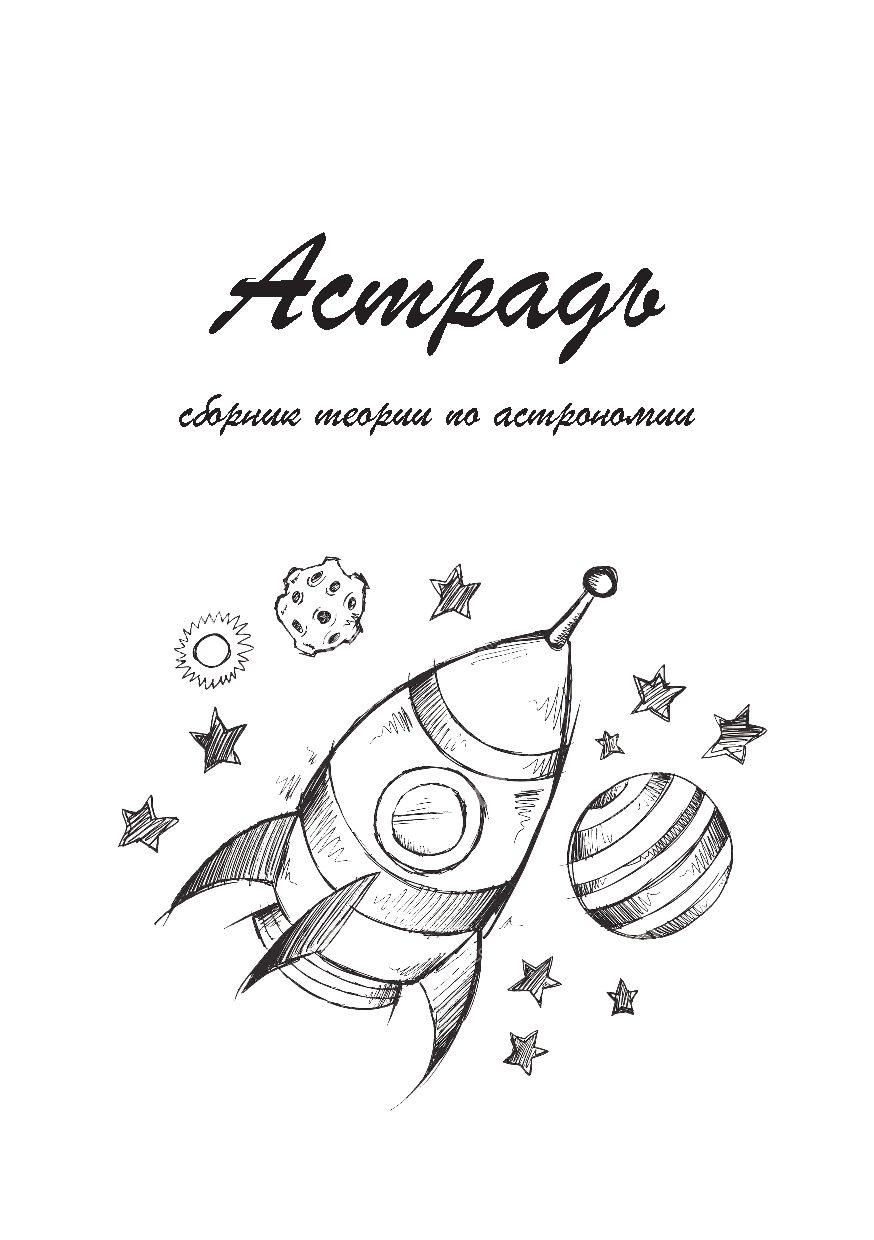
\includegraphics[width=0.95\tw]{sys/cover.pdf}\\[1pc]
{\scshape Beograd, Srbija \\ \year}	
\end{center}

\setcounter{tocdepth}{2}
{
	\small 
	\renewcommand{\baselinestretch}{ 0.95 } 
	\tableofcontents 
	\label{toc}
	\renewcommand {\baselinestretch}{ 1.02 }
}
\section{Небесная механика}
\subsection{Расстояние и размеры}
\term{Астрономическая единица}~--- единица измерения расстояния в астрономии, 
равная большой полуоси орбиты Земли.\begin{equation}
	1~\au = 149\:597\:870\:700~\text{м} \simeq 1.5 \times 10^{11}~\text{м}
\end{equation}

\term{Годичный параллакс} ($\pi$) объекта~--- это угол, под которым видно 
орбиту Земли из окрестностей данного объекта. Применяется к объектам вне 
Солнечной системы. \begin{equation}
	\sin \pi = \frac{a_\oplus}{r},
	\label{eq:parallax-sin}	
\end{equation}
где $a_\oplus$~--- большая полуось орбиты Земли и $r$~--- расстояние до объекта 
имеют одинаковые единицы измерений. Учитывая малость угла $\pi$, можно заменить $\sin\pi$ на $\pi$ в \eqref{eq:parallax-sin}, получим \begin{equation}
	\pi = \frac{a_\oplus}{r}
	\label{eq:parallax}
\end{equation} 

\begin{figure}[h!]
\centering
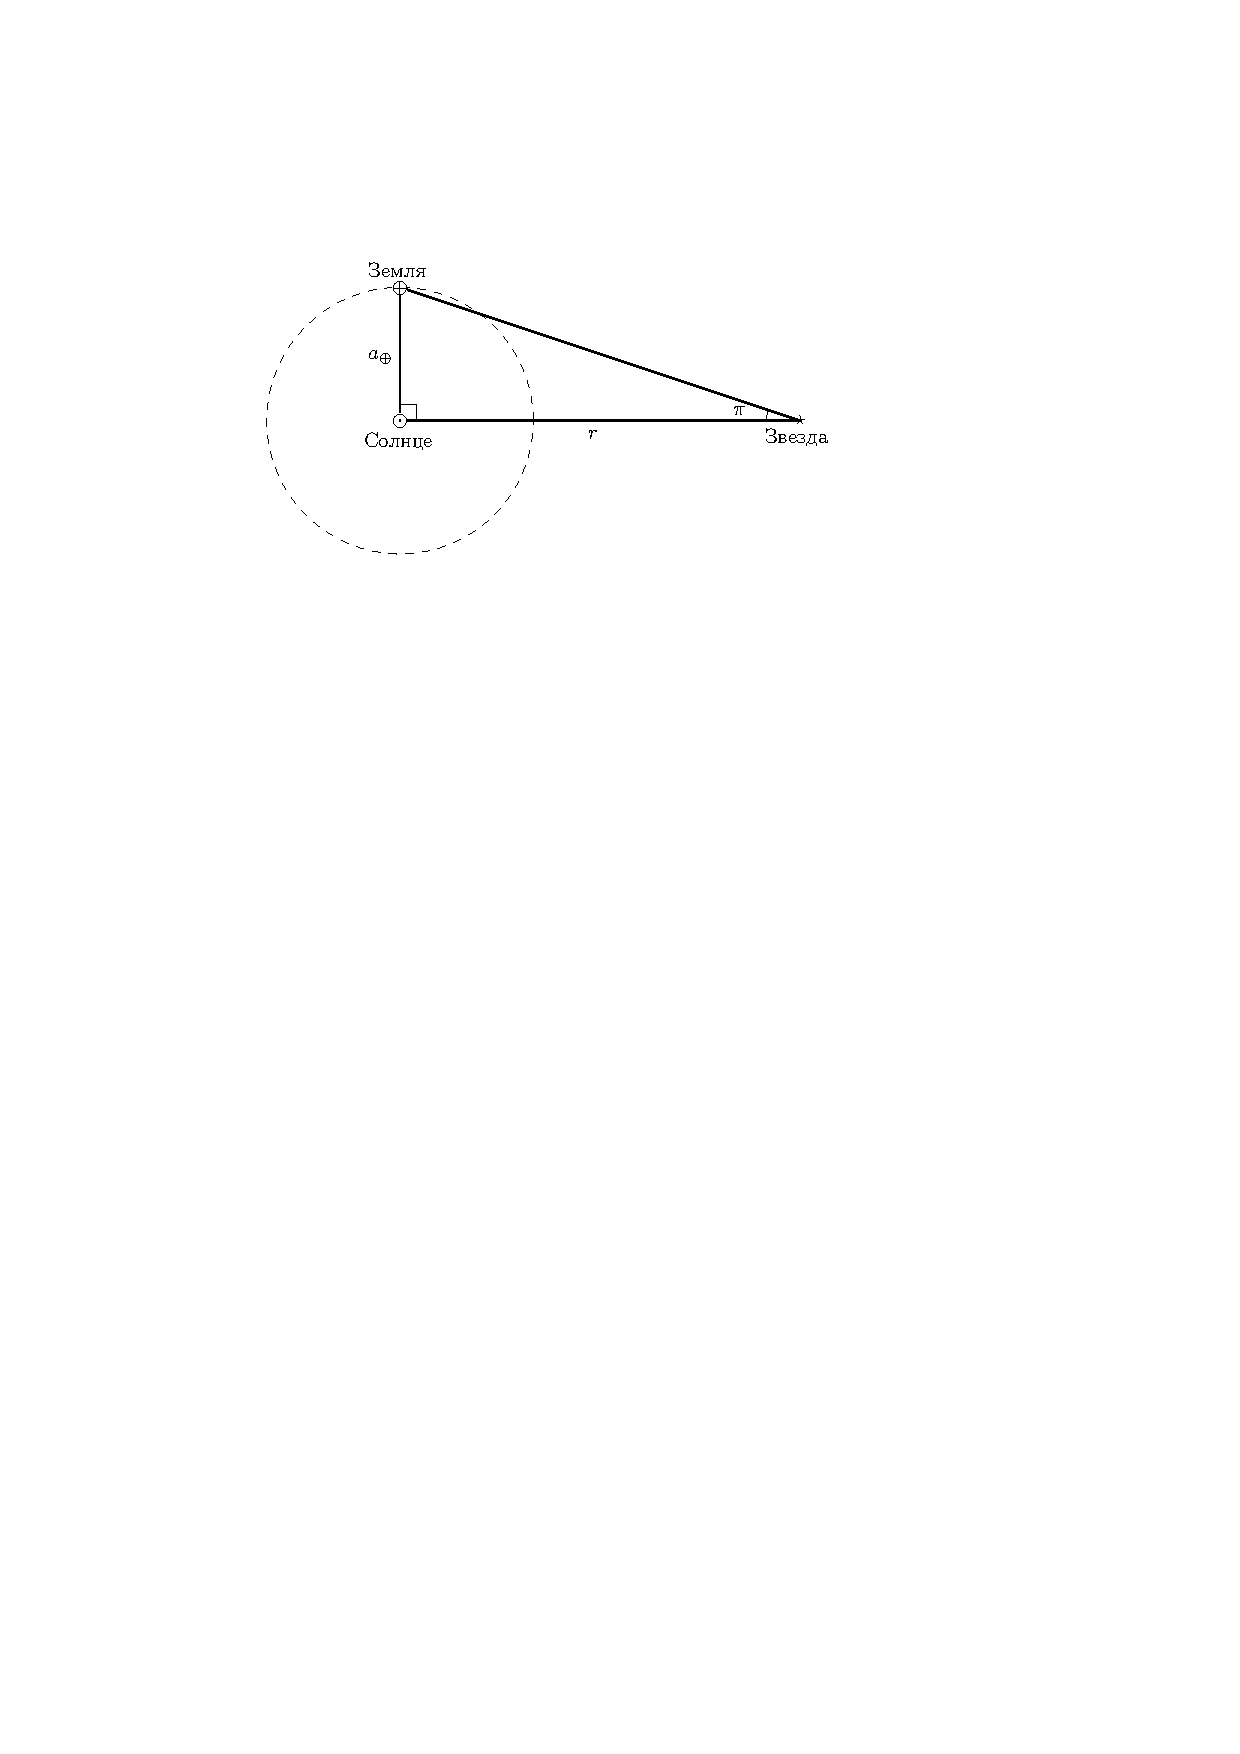
\includegraphics[width = 0.7\tw]{parallax.pdf}
\caption{Схема годичного параллакса}
\end{figure}

Расстояние $r$, с которого большая полуось орбиты Земли $a_\oplus$ видна под углом $\pi = 1''$ называется \term{1 парсеком}. Так как \begin{equation}
	1~\text{рад} = \frac{180^\circ}{\pi} \simeq  3 438' \simeq 206265'' 
\quad \Longrightarrow \quad \mathsf{1~\text{\sffamily пк} = 
206265~\text{\sffamily а.\,е.}},
\end{equation} 
следовательно, записывая большую полуось орбиты Земли в \au, а расстояние до звезды в парсеках, получаем параллакс в секундах. Таким образом имеем следующую формулу:\begin{equation}
	r_\text{пк} = \frac{1~\au}{\pi''},
\end{equation}
где $\pi''$ --- годичный параллакс объекта в секундах дуги.


\term{Угловой размер объекта}~--- это угол, под которым видно объект. Для астрономии наиболее актуален угловой размер сферически симметричных объектов, для которых угловой размер (диаметр) определяется, как
\begin{equation}
\rho = 2 \arcsin \frac{R}{r}, 
\end{equation}
где $R$~--- радиус объекта, а $r$~--- расстояние до него.

\begin{figure}[h!]
\centering
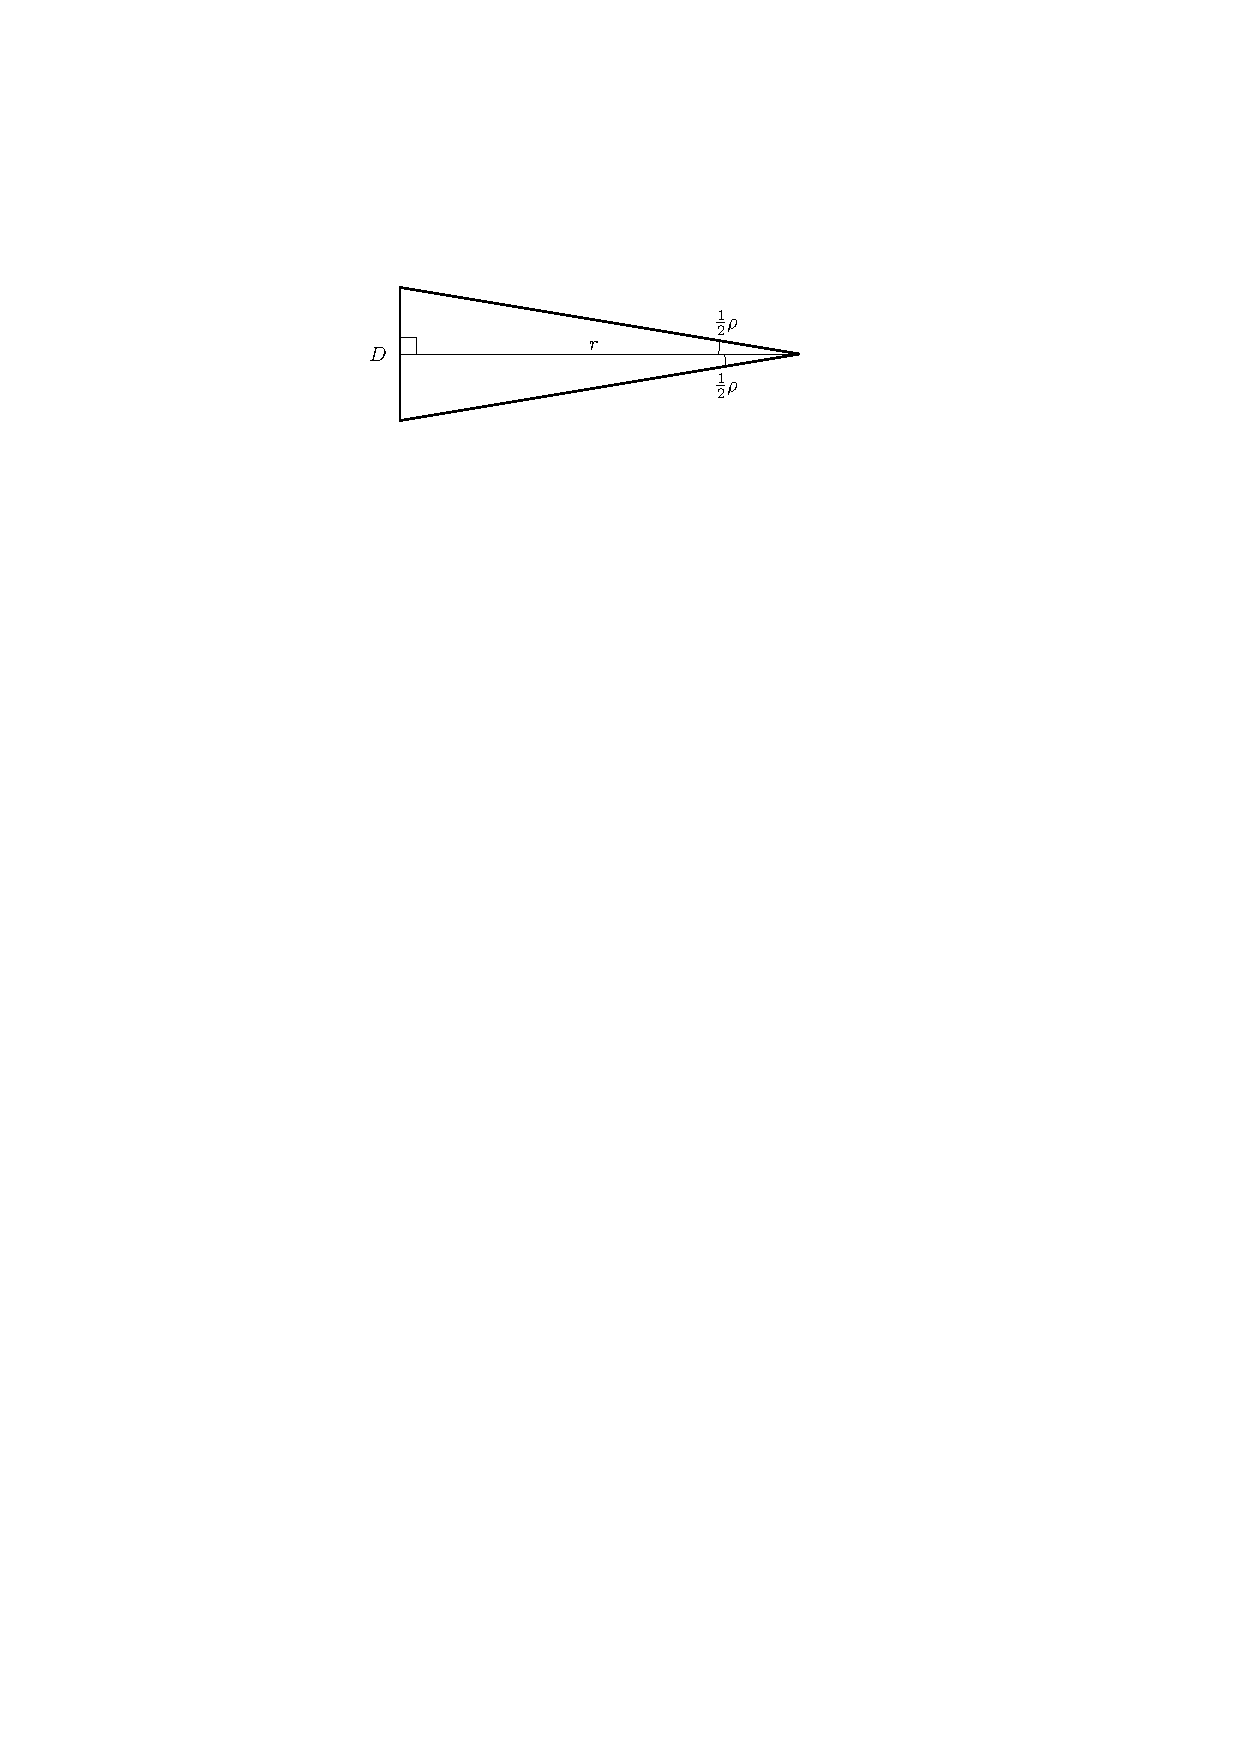
\includegraphics[width = 0.6\tw]{angle-size}
\caption{Угловой размер}
\end{figure}

В случаем, когда $r$ много больше размера объекта $R$, то есть $r\gg R$, можно воспользоваться приближением для малых углов, тогда \begin{equation}
	\rho \simeq \frac{2 R}{r}
\end{equation}

\term{Горизонтальный параллакс $(p)$}~--- это угол, под которым видно радиус Земли, при положении светила на горизонте.
\begin{equation}
\sin p=\frac{R_\oplus}{r},
\end{equation}
где $R_\oplus$~--- радиус Земли, $p$~--- горизонтальный параллакс, $r$~--- 
расстояние до объекта.

\begin{figure}[h!]
\centering
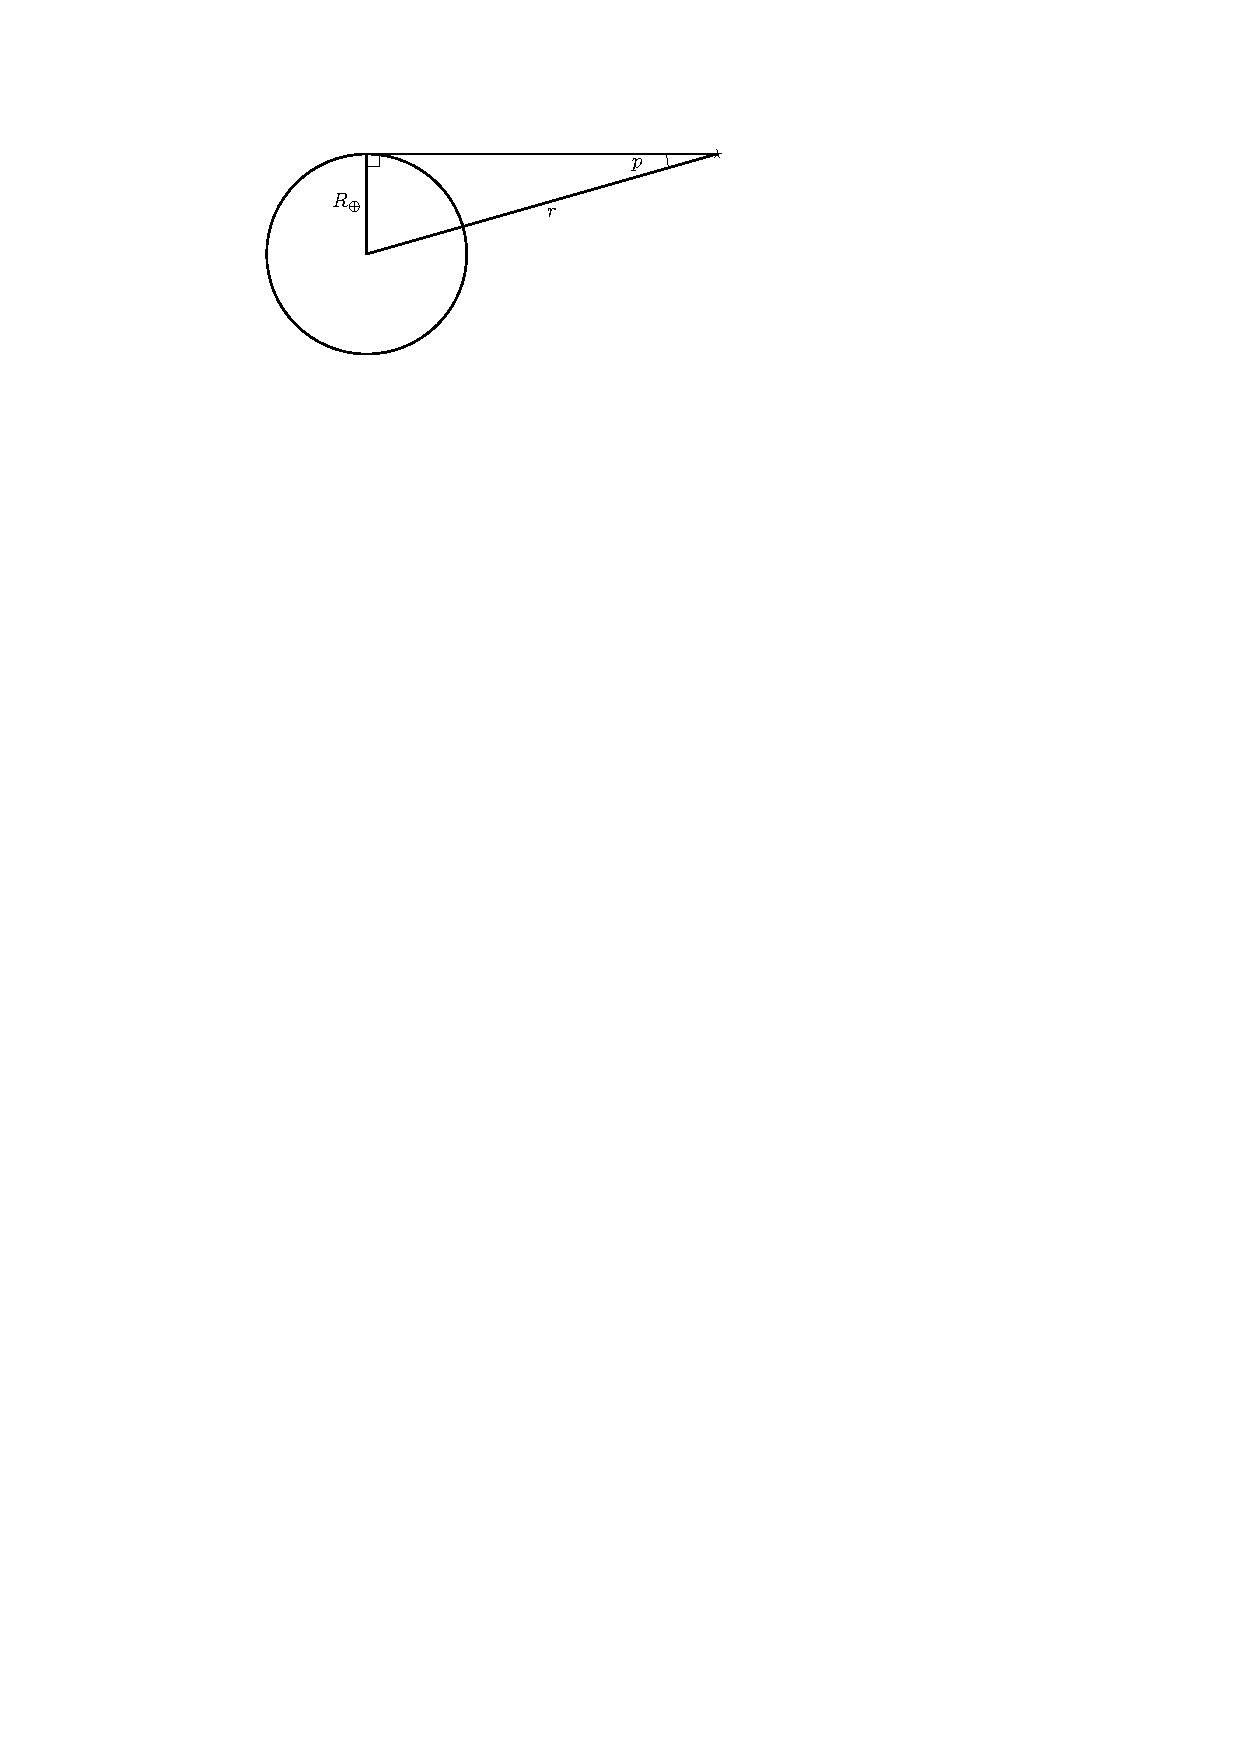
\includegraphics[width = 0.6\textwidth]{parallax-horiz}
\caption{Горизонтальный параллакс}
\end{figure}

\term{Правило Тициуса-Боде} --- эмпирическая формула приблизительно описывающая 
радиусы орбит планет от Солнца:
\begin{equation}r=\frac{3\cdot 2^n+4}{10}, \quad tn=-\infty, 0, 1, 2...
\end{equation}


\subsection{Закон всемирного тяготения}
Согласно \imp{закону всемирного тяготения}, сила притяжения 
между двумя точечными телами с массами $M$ и $m$,
находящимися на расстоянии $r$ выражается следующим
образом:\begin{equation}
	F=\frac{GMm}{r^2}, \label{eq:grav-law}
\end{equation}
где $G\simeq 6.67\cdot 10^{-11}~\text{м}^3 / 
\left( \text{кг} \cdot \text{с}^2 \right)$ --- 
\term{гравитационная постоянная}.

\term{Гравитационный потенциал} поля точечной (или сферически 
симметричной) массы $M$ на расстоянии $r$ от нее равен
работе, которую необходимо затратить, чтобы принести
единичную массу с бесконечности в данную точку. Так как
гравитационные силы между двумя массами --- это силы 
притяжения, то эта работа отрицательна. Данная
величина также является \term{потенциальной энергией} точечной
массы на расстоянии $r$ от массы $M$, а выражение для нее имеет 
следующий вид:\begin{equation}
U=-\frac{GM}{r}
\end{equation}

Напряженность гравитационного поля $dU/dr$ часто называют 
\term{ускорением свободного падения} $g$, где
\begin{equation}
	g = \frac{GM}{r^2}
	\label{eq:g}
\end{equation}
Тогда (\ref{eq:grav-law}) можно записать, как \begin{equation}
	F = mg
\end{equation}
%\begin{table}[h!]
%\centering
%\begin{tabular}{|c|c|c|c|}
%\hline 
%{\bfseries Планета} & $\mathbf{g}$, 
%{\bfseries м/$\text{\bfseries c}^2$} 
%& {\bfseries Планета} & $\mathbf{g}$, 
%{\bfseries м/$\text{\bfseries c}^2$}\\
%\hline
%Солнце & 276. & Марс & 3.73\\
%\hline
%Меркурий & 3.73 & Юпитер & 25.9\\
%\hline
%Венера & 8.87 & Сатурн & 11.2\\
%\hline
%Земля & 9.82 & Уран & 9.01\\
%\hline
%Луна & 1.63 & Нептун & 11.3\\
%\hline
%\end{tabular}
%\caption{Ускорение свободного падения на поверхности тел 
%солнечной системы}
%\end{table}

\subsection{Закон сохранения энергии и типы орбит}
Для движения тела c массой $m$ в гравитационном  в поле тела 
с массой \linebreak $M\gg m$ со скорость $v$ на расстоянии $r$ от 
гравитационного центра справедливо следующее соотношение: 
\begin{equation}
\frac{m v^2}{2}-\frac{GM m }{r}=E_0,
\end{equation}
где $E_0$ --- постоянная величина, если на тело не действуют
внешние силы кроме силы притяжения к центральному телу, 
равная сумме кинетической и потенциальной энергии тела. Данное равенство принято называть \term{законом сохранения энергии} для тела, движущегося в поле консервативных (потенциальных) сил.

\begin{wrapfigure}[11]{l}{.5\tw}
	\centering
	\vspace{-1.2pc}
	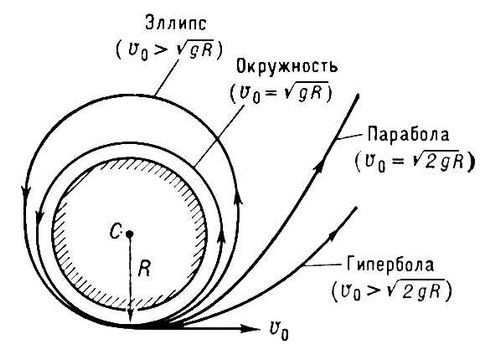
\includegraphics[width = 0.5\tw]{Space-speed}
	\caption{Возможные траектории тела \label{pic:orbits}}
\end{wrapfigure}
Если $E_0>0$, то траектория тела~--- \imp{гипербола}, 
ветви которой асимптотически приближаются к двум прямым. Стоит заметить,
что на бесконечно большом удалении тела с массой $m$ от массивного тела
его скорость остается положительной, так как суммарная энергия $E_0$ 
больше нуля.

Если $E_0=0$, то траектория тела~--- \imp{парабола}. При стремлении
расстояния $r$ между телами к бесконечности, скорость тела с стремится к нулю.

Отсюда становится очевидно, что на параболической и гиперболический
 траекториях движение тела не ограничено (инфинитно). 

Если $E_0<0$, то траектория тела~--- \imp{эллипс}. При 
эллиптической траектории движение ограничено (финитно), так как малое тело
не может бесконечно удалять с неотрицательной скоростью по причине того,
что суммарная энергия меньше нуля.

На Рис.\,\ref{pic:orbits} представлены примеры возможных траекторий тела 
относительно центрального (точка C). При $v_0 > v_{2}$ --- тело движется 
по гиперболе, при $v_0 = v_{2}$ --- по параболе, 
а при $v_0 < v_{2}$ --- по эллипсу.\\

\term{Первая космическая скорость} --- минимальная скорость, необходимая для 
того, чтобы маломассивное тело стало искусственным спутником центрального тела.
\begin{equation}v_1=\sqrt{\frac{GM}{R}}
\end{equation}
где $M$ --- масса массивного тела. Отсюда несложно получить выражение для
скорости искусственного небесного тела на высоте 
$h$.\begin{equation}v_h=\sqrt{\frac{GМ}{R+h}}=\sqrt{\frac{gR^2}{R+h}}
\end{equation}

\term{Параболическая} или \term{вторая космическая скорость} --- 
минимальная скорость, необходимая для того, чтобы маломассивное тело преодолело 
гравитационное притяжение центрального тела и покинуло замкнутую орбиту вокруг 
последнего. Выражение для которой имеет следующий вид:\begin{equation}
v_{2}=\sqrt{\frac{2GM}{r}}
\end{equation}

Для стабильной системы, частный случай~--- тело на круговой орбите, справедлива 
\term{теорема о вириале}:
\begin{equation}
2 \langle T\rangle 
= -\sum _{{k=1}}^{N}\langle {F}_{k}\cdot {r}_{k}\rangle 
= \langle U \rangle
\end{equation}

Где $\langle T\rangle$ --- средняя полная кинетическая энергия, $F_k$ --- сила, 
действующая на $k$-ю частицу. Другими словами, удвоенная средняя полная 
кинетическая энергия $T$ равна средней полной потенциальной энергии $U$. 

Применяя теорему о вириале для тела, обращающегося по круговой орбите можно 
получить выражения для первой космической скорость.
%\begin{table}[h!]
%\centering
%\begin{tabular}{|c|c|c|}
%\hline
%\textbf{Планета} & $\mathbf{v_1}$,~\textbf{км/c} & 
%$\mathbf{v_2}$,~\textbf{км/c}\\
%\hline
%Солнце & 436,8 & 617,7\\
%\hline
%Меркурий & 3,0 & 4,3\\
%\hline
%Венера & 7,4 & 10,5\\
%\hline
%Земля & 7,9 & 11,2\\
%\hline
%Луна & 1,7 & 2,4\\
%\hline
%Марс & 3,5 & 5,0\\
%\hline
%Юпитер & 42,0 & 59,5\\
%\hline
%Сатурн & 25,1 & 35,5\\
%\hline
%Уран & 15,0 & 21,3\\
%\hline
%Нептун & 16,6 & 23,5\\
%\hline
%\end{tabular}
%\caption{$v_1$ и $v_2$ на некоторых телах Солнечной системы}
%\end{table}





\subsection{Законы Кеплера}
\term{I-ый закон:} Все планеты движутся по 
эллиптическим орбитам, в одном из фокусов которых 
находится Солнце.\\

\term{ II-ой закон:} Радиус-вектор планеты за 
равные промежутки времени заметает равные площади.
\begin{equation}
\frac{dS}{dt}=const
\end{equation}
\term{III-ий закон:} Квадраты периодов обращения планет 
относятся, как кубы больших полуосей их орбит.
\begin{equation}
\frac{T^2_1}{T^2_2}=\frac{a^3_1}{a^3_2},
\end{equation}
где $a$ --- большая полуось, $T$ --- период обращения.
\begin{figure}[h!]
\begin{minipage}[b]{0.5\textwidth}
\centering
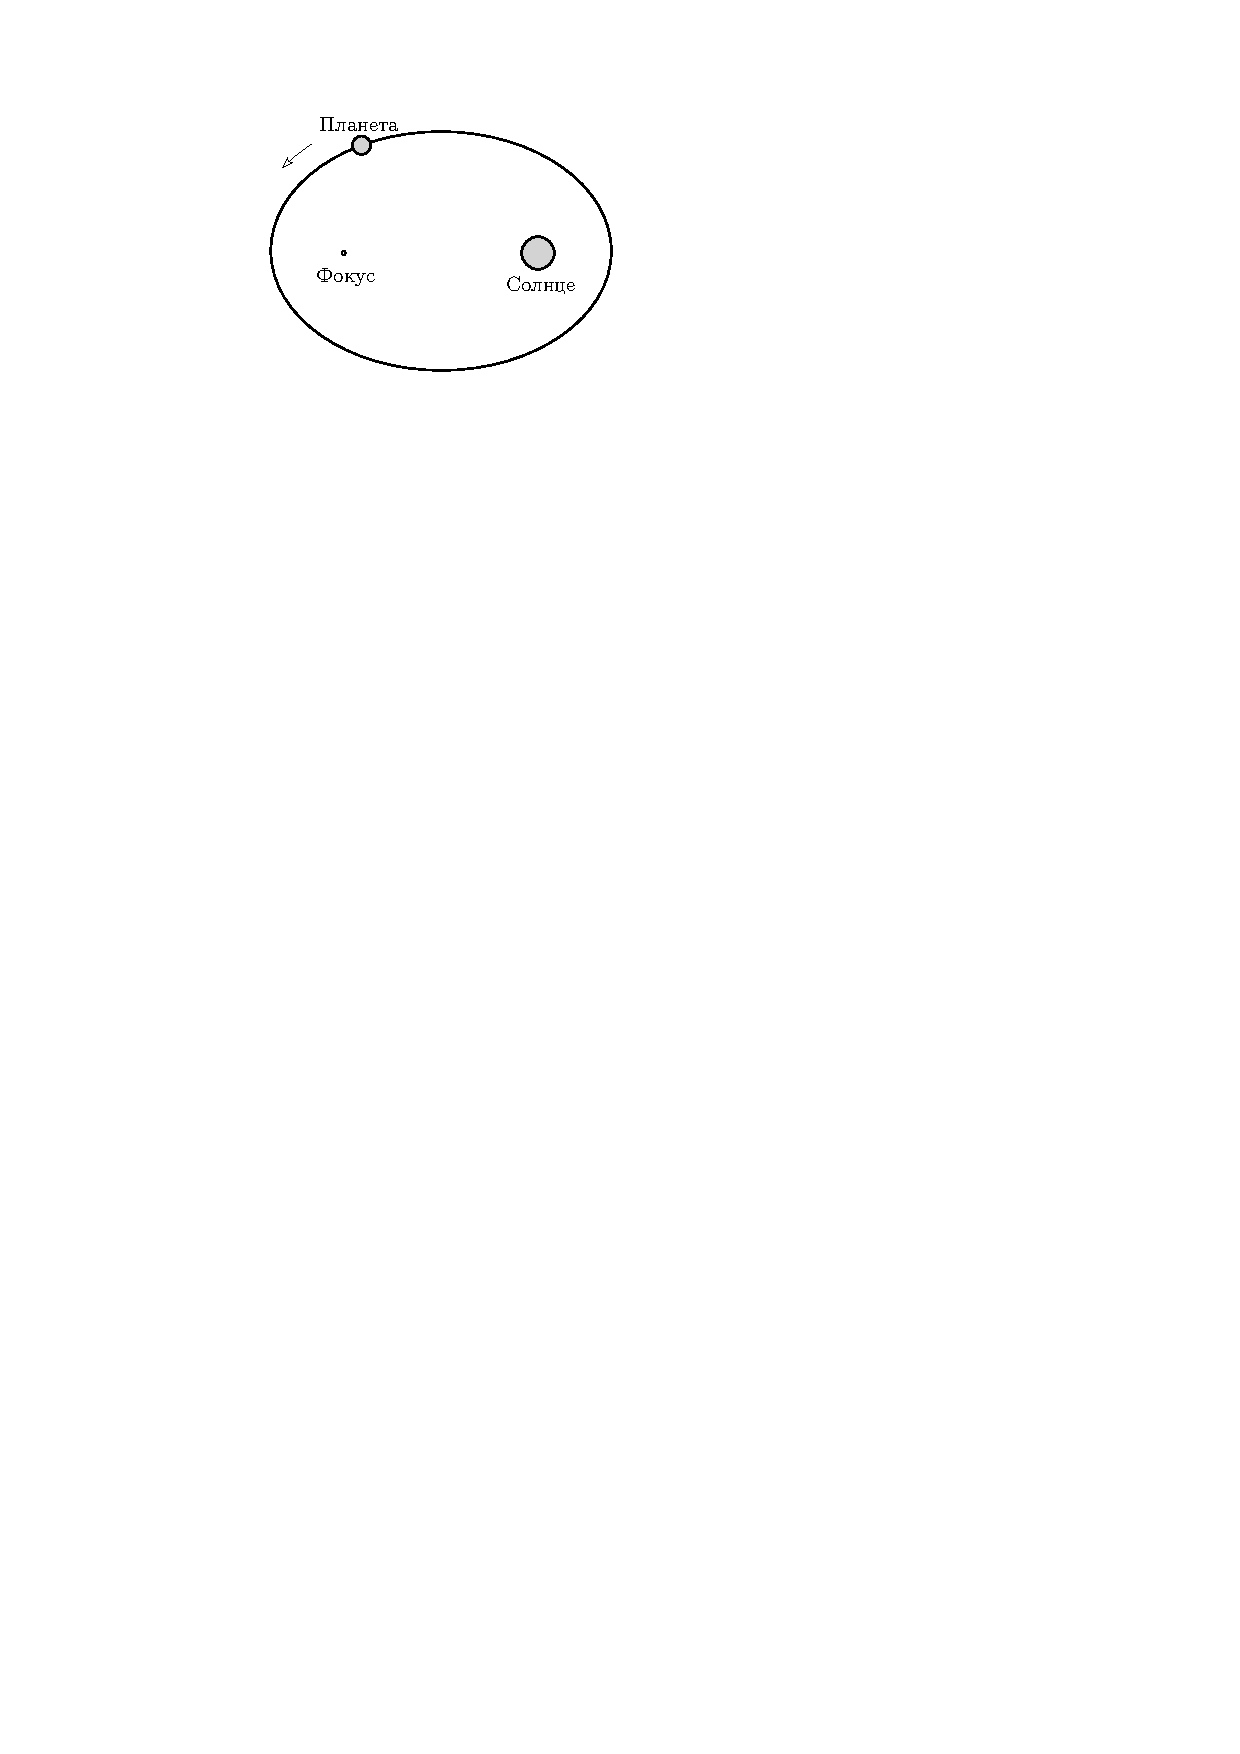
\includegraphics[width = 0.84\textwidth]{first-kepler}
\caption{Первый закон Кеплера}
\end{minipage}
\begin{minipage}[b]{0.5\textwidth}
\centering
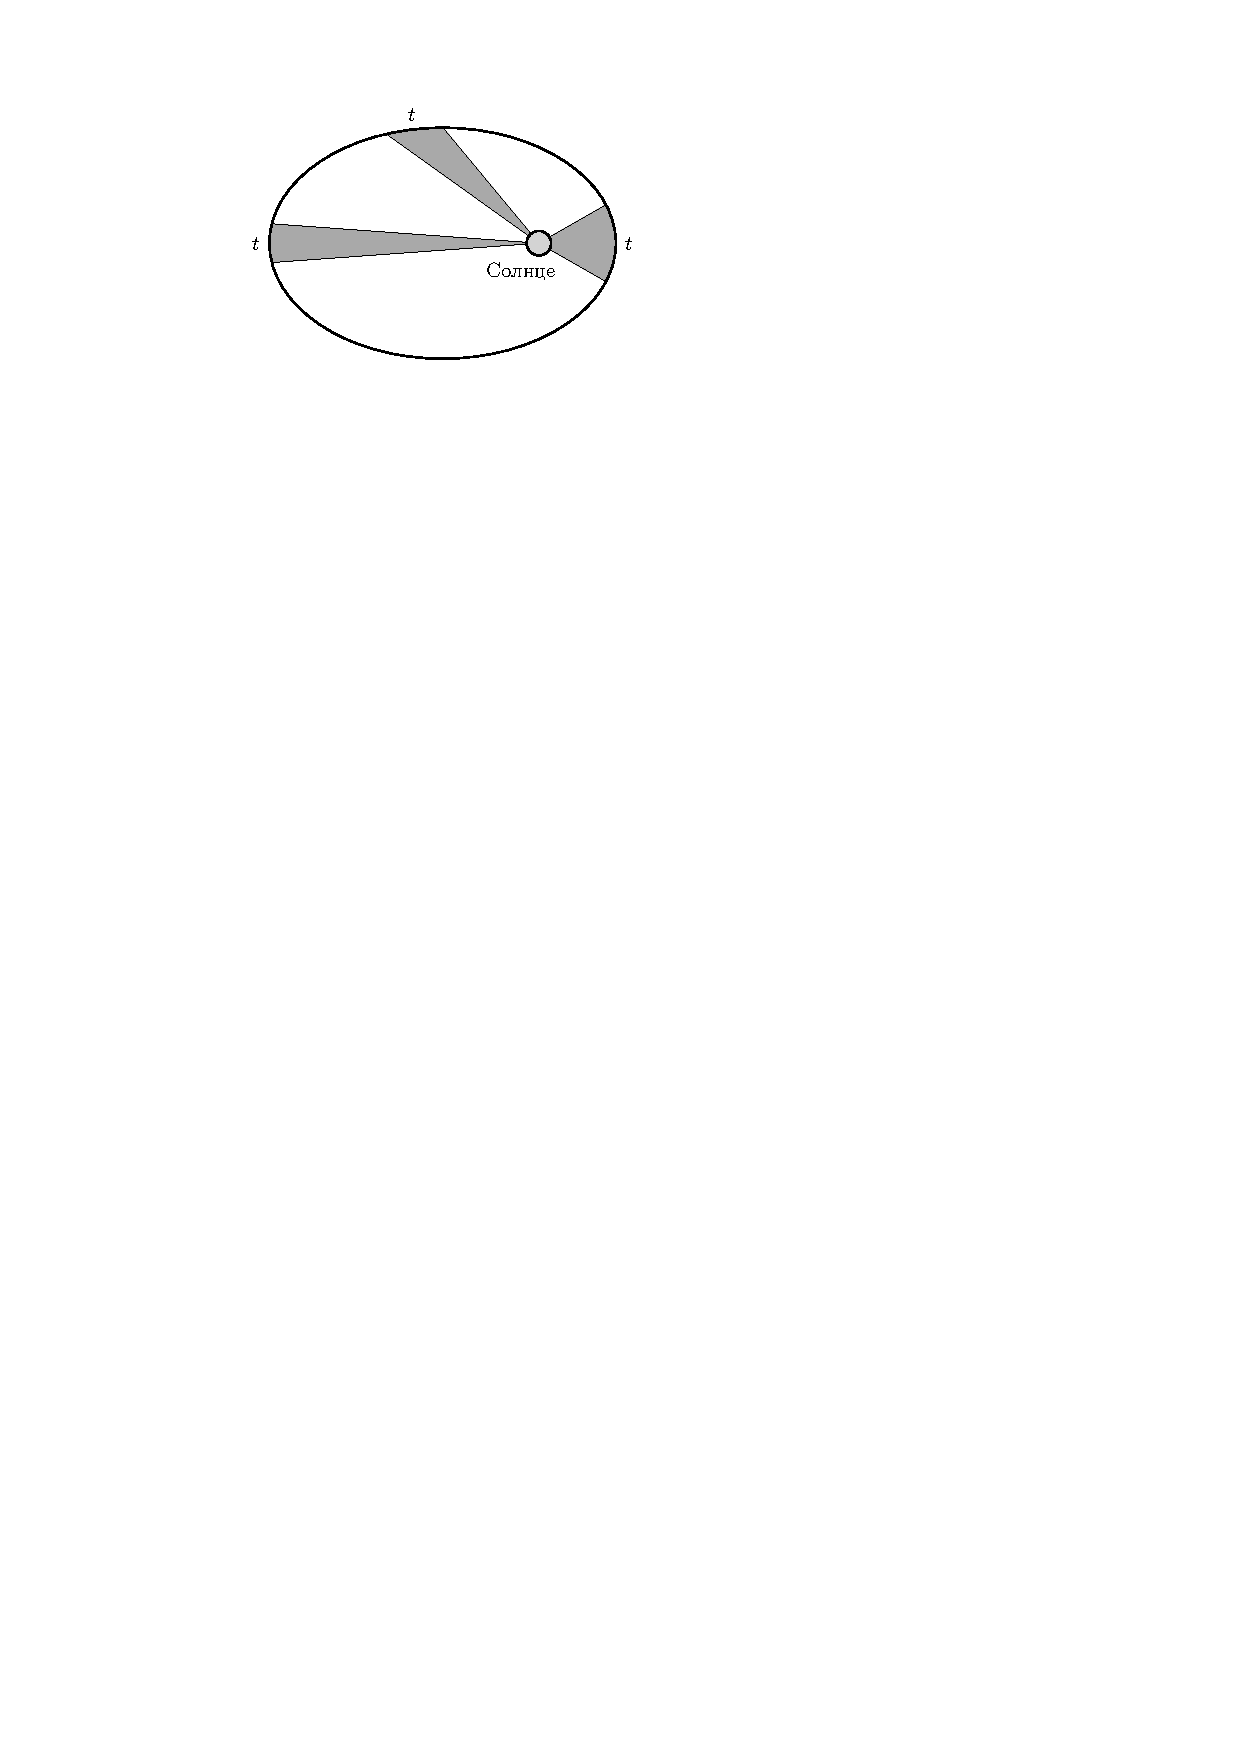
\includegraphics[width = 0.972\textwidth]{second-kepler}
\caption {Второй закон Кеплера}
\end{minipage}
\end{figure}

\term{Обобщённый} Ньютоном \term{III-ий закон Кеплера} имеет следующий вид:
\begin{equation}
\frac{T^2_1( M_1 + m_1)}{T^2_2( M_2 + m_2 )}=\frac{a^3_1}{a^3_2} \quad \Longleftrightarrow \quad 
	\frac{T^2}{a^3} = \frac{4 \pi^2}{G ( M + m )},
\end{equation}
где $M_1$ и $M_2$~--- массы центральных тел, $m_1$ и 
$m_2$~--- массы обращающихся вокруг них тел. Так как массы планет 
$m$ много меньше массы звезды $M$, то $M + m \simeq M$.

\subsection{Движение по орбите}

\term{Закон сохранения момента импульса}:  векторная сумма всех моментов 
импульса относительно выбранной оси для замкнутой системы тел, которая остается 
постоянной, пока суммарный момент $\vec{M}_\Sigma$ внешних сил, действующих на систему, равен нулю. Иначе
\begin{equation}
\vec{L}_\Sigma \equiv \sum\limits_{i=1}^{n} \left[ \vec{r} \times m \vec{v} \right] = const.
\end{equation}

Закон сохранения момента импульса справедлив как для движения по эллипсу, так и по
гиперболе и параболе. Следствием этого закона и закона сохранения энергиии 
является \imp{интеграл энергии}~--- формула для скорости тела в точке орбиты, удалённой на расстояние~$r$ от центрального тела с массой $M$:
\begin{equation}
v = \sqrt{ GM \left( \frac{2}{r} - \frac{1}{a} \right)}.
\label{eq:int-energy}
\end{equation}

Из \eqref{eq:int-energy} для апоцентра и перицентра можно заключить следующее:
\begin{equation}v_{\text{аф}}=\sqrt{\frac{GM}{a}} \sqrt{\frac{1-e}{1+e}}
\quad\quad\quad v_{\text{пер}}=\sqrt{\frac{GM}{a}}\sqrt{\frac{1+e}{1-e}}
\end{equation}

Согласно \eqref{eq:int-energy} и \eqref{eq:ellipse-pol-eq} для скорости тела в произвольной точке орбиты справедливо выражение
\begin{equation}
v = \sqrt{\frac{GM}{p}\cdot(1 + 2 e \cos \nu + e^2)},
\end{equation}
где $\nu$~--- истинная аномалия, а $p$~--- фокальный параметр.

\subsection{Кеплеровы элементы орбиты}

\term{Кеплеровы элементы} --- шесть элементов орбиты, определяющие положение
\begin{wrapfigure}[14]{r}{0.45\tw}
	\centering
	\vspace{-1pc}
	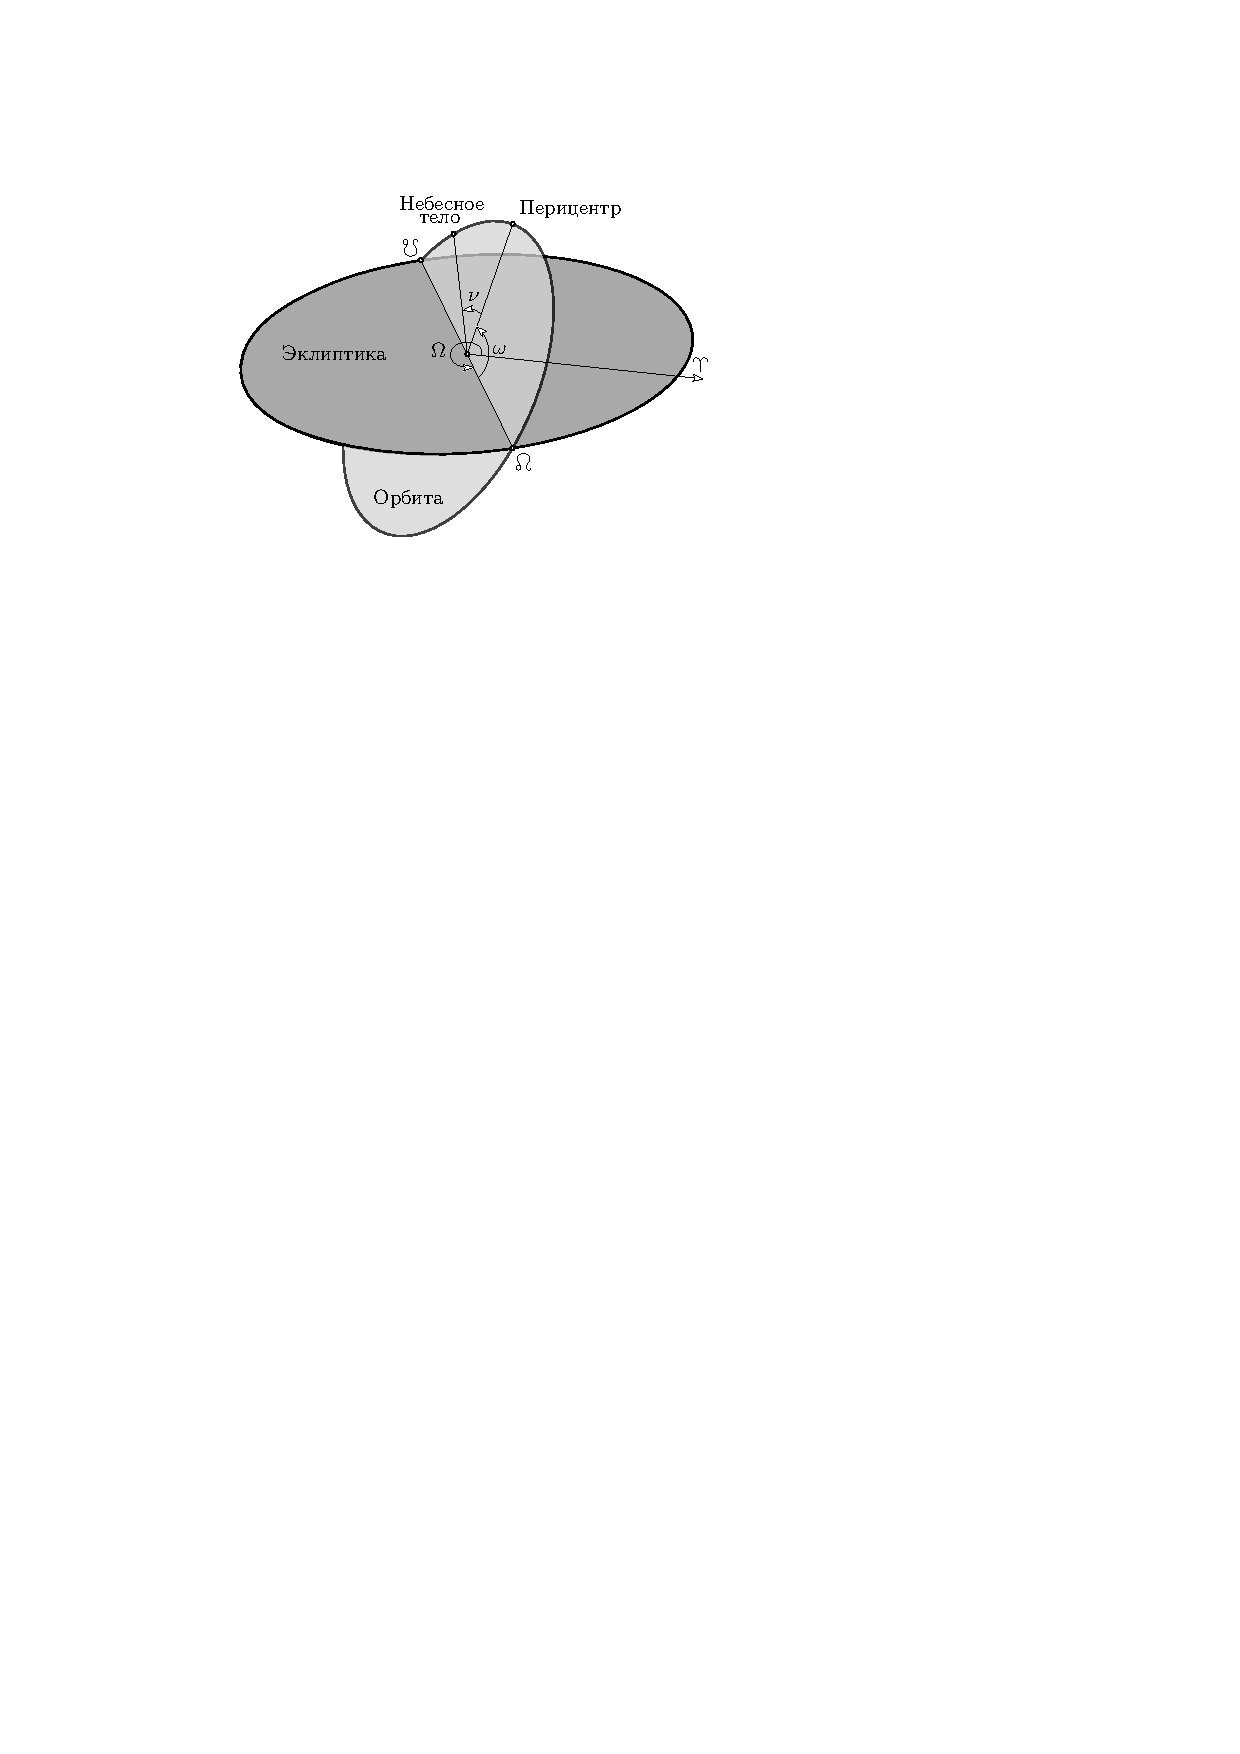
\includegraphics[width=.45\tw]{orbit-elem}
	\captionof{figure}{Кеплеровы элементы орбиты}
	\label{fig:orb-elem}
\end{wrapfigure}
небесного тела в пространстве в задаче двух тел: \imp{большая полуось} ($a$), \imp{эксцентриситет} ($e$), \imp{наклонение} ($i$), \imp{аргумент перицентра} ($\omega$), \imp{долгота восходящего узла} ($\Omega$), \imp{средняя аномалия} ($M_0$). Первые два определяют форму орбиты, третий, четвёртый и пятый~--- ориентацию плоскости орбиты по отношению к базовой системе координат, связанной с эклиптикой, последний~--- положение тела на орбите~(см.~Рис.\,\ref{fig:orb-elem}).

\term{Наклонение}~--- это угол между плоскостью орбиты небесного тела и плоскостью эклиптики.

\term{Аргумент перицентра}~--- угол между направлениями на восходящий узел орбиты и на перицентр при наблюдении из притягивающего центра.

\term{Долгота восходящего узла}~--- угол в плоскости эклиптики между направлением на точку весеннего равноденствия и восходящий узел орбиты. Отсчитывается против часовой стрелки от направления на точку весеннего равноденствия.

\term{Средняя аномалия} для тела, движущегося по невозмущённой орбите~--- произведение его среднего движения и интервала времени после прохождения перицентра.

\term{Узлы орбиты}~--- точки пересечения орбиты и плоскости эклиптики. \imp{Восходящий узел}~--- точка, в которой тело пересекает плоскость эклиптики при движении в северноим направлении, а \imp{нисходящий}~--- в южном.

\term{Истинная аномалия}~($\nu$)~--- угол между радиус-вектором и направлением на перицентр.
\subsection{Точки Лагранжа}

\term{Точки Лагранжа}~--- точки, во вращающейся системе из двух массивных тел,
\begin{wrapfigure}[14]{l}{0.48\tw}
	\centering
	\vspace{-.5pc}
	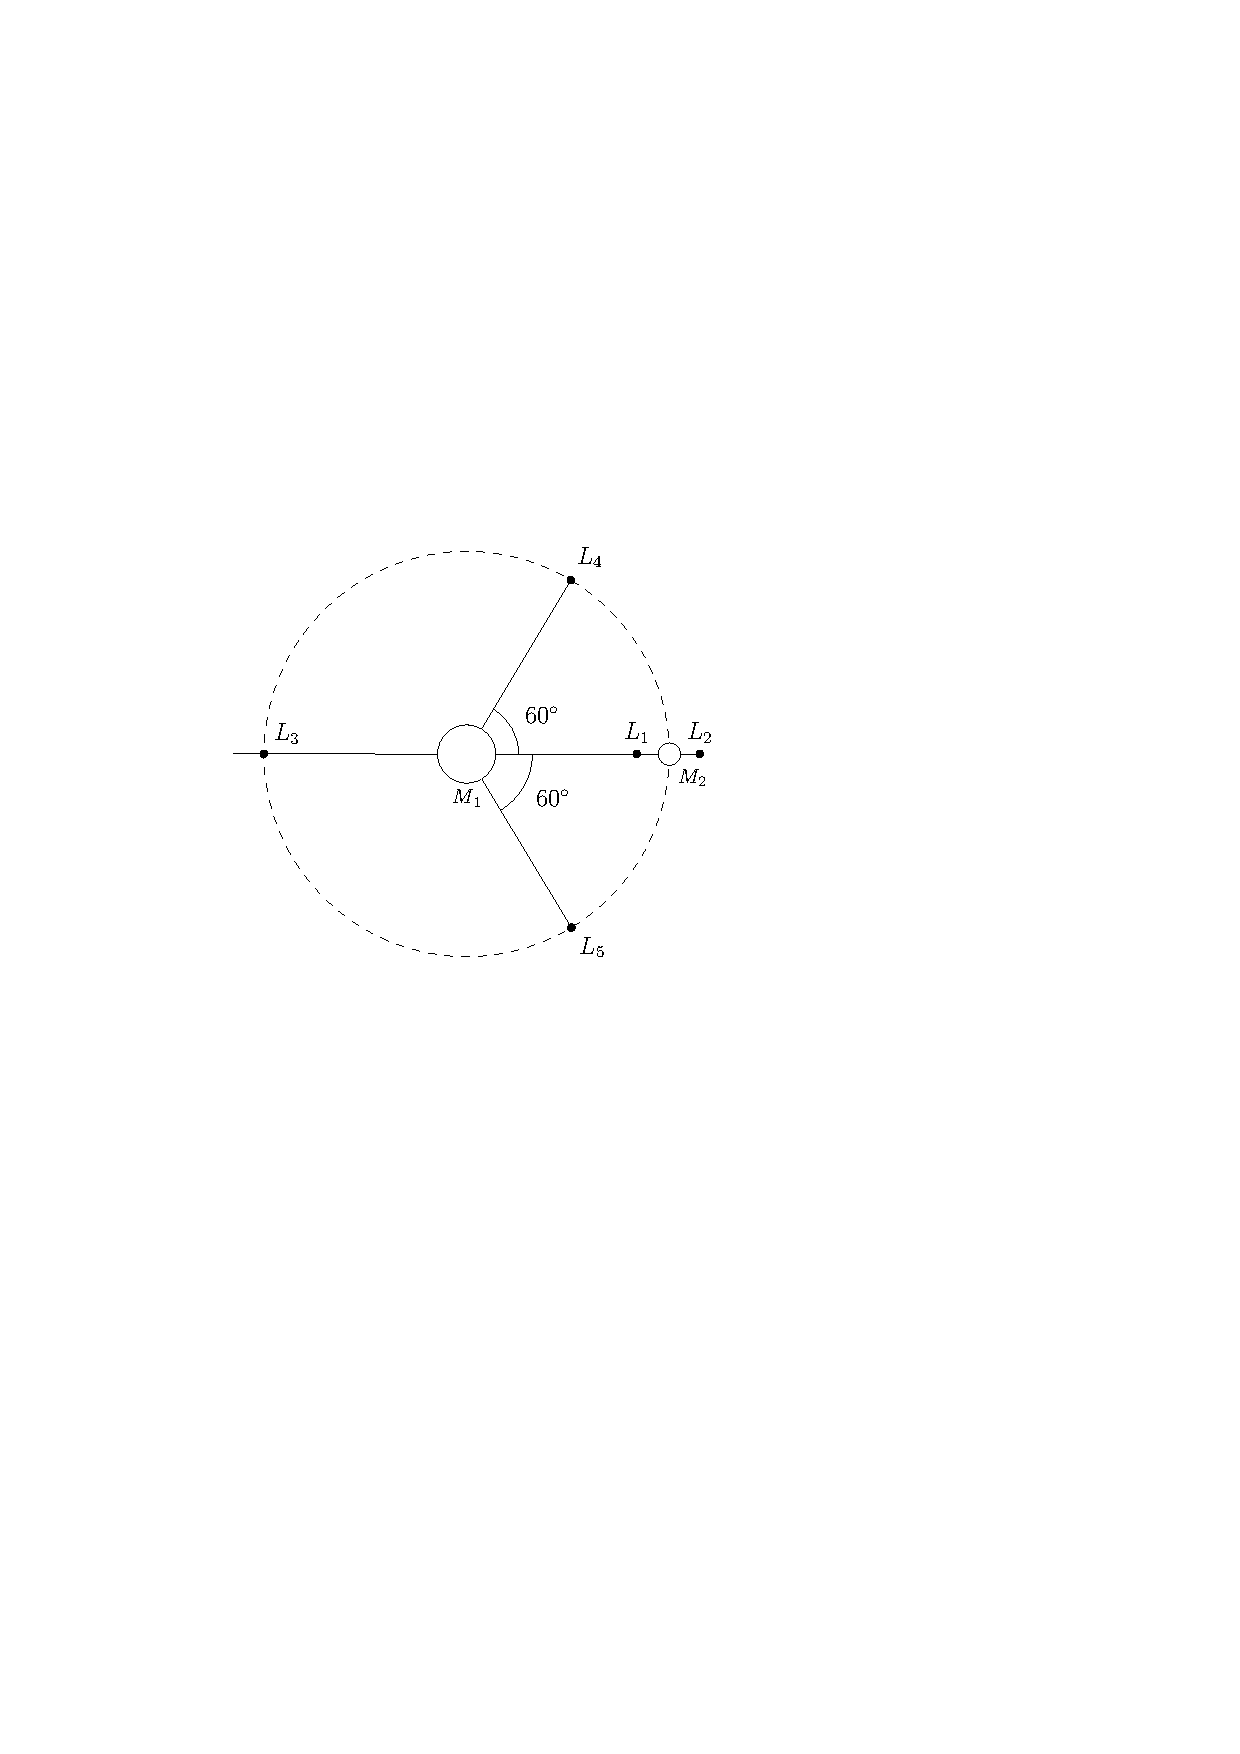
\includegraphics[width = .48\tw]{lagr-points}
	\captionof{figure}{Точки Лагранжа}
	\label{pic:larg-points}	
\end{wrapfigure}
в которых третье тело с пренебрежимо 
малой массой, не испытывающее воздействие никаких 
других сил, кроме гравитационных, со стороны двух 
первых тел, может оставаться неподвижным относительно 
этих тел. В этих точках гравитационные силы, 
действующие на малое тело, уравновешиваются силами инерции.

Точки $L_1$, $L_2$ и $L_3$ лежат на одной прямой, 
соединяющей два массивных тела. Точки $L_4$ и $L_5$ 
образуют равносторнние треугольники с массивными 
телами.

Для расстояний до точек $L_1$, $L_2$ и $L_3$ от 
центра масс системы справедливы следующие выражения:
\begin{equation}r_1=R\left(1-\sqrt[3]{\frac{\alpha}
{3}}\right), \quad r_2=R\left(1+\sqrt[3]{\frac{\alpha}
{3}}\right), \quad r_3=R\left(1+\frac{5}{12}\alpha\right),
\end{equation}
где $\alpha=M_2 / (M_1 + M_2)$, $R$~--- расстояние между 
телами, $M_1$ --- масса более массивного тела, $M_2$
 --- масса второго тела.

Если $M_2 \ll M_1$, то точки $L_1$ и $L_2$ находятся 
примерно на одинаковом расстоянии от тела $M_2$, равном
\begin{equation}
r\approx R\sqrt[3]{\frac{M_2}{3M_1}}.
\end{equation}

Расстояния от центра масс системы до точек $L_4$ и $L_5$ в координатной системе с центром координат в центре масс системы рассчитываются по  формулам
\begin{equation}
	 r_4 = \left ( \frac{R}{2} \cdot \frac{M_1-M_2}{M_1+M_2} ,   \frac{\sqrt{3}R}{2} \right ), \quad r_5 = \left ( \frac{R}{2} \cdot \frac{M_1-M_2}{M_1+M_2} ,   -\frac{\sqrt{3}R}{2} \right ). 
\end{equation}
\subsection{Приливы и отливы}

\term{Приливы и отливы}~--- периодические вертикальные колебания уровня океана или моря, являющиеся результатом как изменения положения Луны, так Солнца. Хотя силы тяготения Солнца почти в 200 раз больше, чем силы тяготения Луны, приливные силы, порождаемые Луной, почти вдвое больше порождаемых Солнцем. Это происходит из-за того, что приливные силы зависят не от величины гравитационного поля, а от степени его неоднородности. Высота приливов зависит от взаимного расположения Луны и Солнца. Наибольший прилив, когда приливообразующие силы Луны и Солнца действуют вдоль одного направления, а наименьший прилив, когда приливообразующие силы Луны и Солнца действуют под прямым углом друг к другу.

Ускорение в центре Земли($T$) считется по следующей формуле: \begin{equation}\omega_T=\frac{GM}{r^2},
\end{equation}
где $M$ --- масса Луны, $r$ --- расстояние между центрами Земли и Луны. Ускорения в точках A и B равны: \begin{equation}
\omega_A = \frac{GM}{(r - R)^2} \quad \text{и} \quad \omega_B = \frac{GM}{(r + R)^2},
\end{equation}
где $R$~--- радиус Земли. Ускорение точки A относительно точки T равно:\begin{equation}
\omega_A - \omega_T = \omega_T \frac{2 r R - R^2}{(r - R)^2},
\end{equation}
так как $R\ll r$, то \begin{equation}
\omega_A - \omega_T = \omega_T \frac{2 R}{r}.
\end{equation}

Под действием лунного притяжения водная оболочка Земли принимает форму 
эллипсоида, который вытянут по направлению к Луне. Близ точек $A$ и $B$ будет 
прилив, а у точек $F$ и $D$ --- отлив (Рис.\,\ref{Ebb_flow}).
\begin{figure}[h!]
\centering
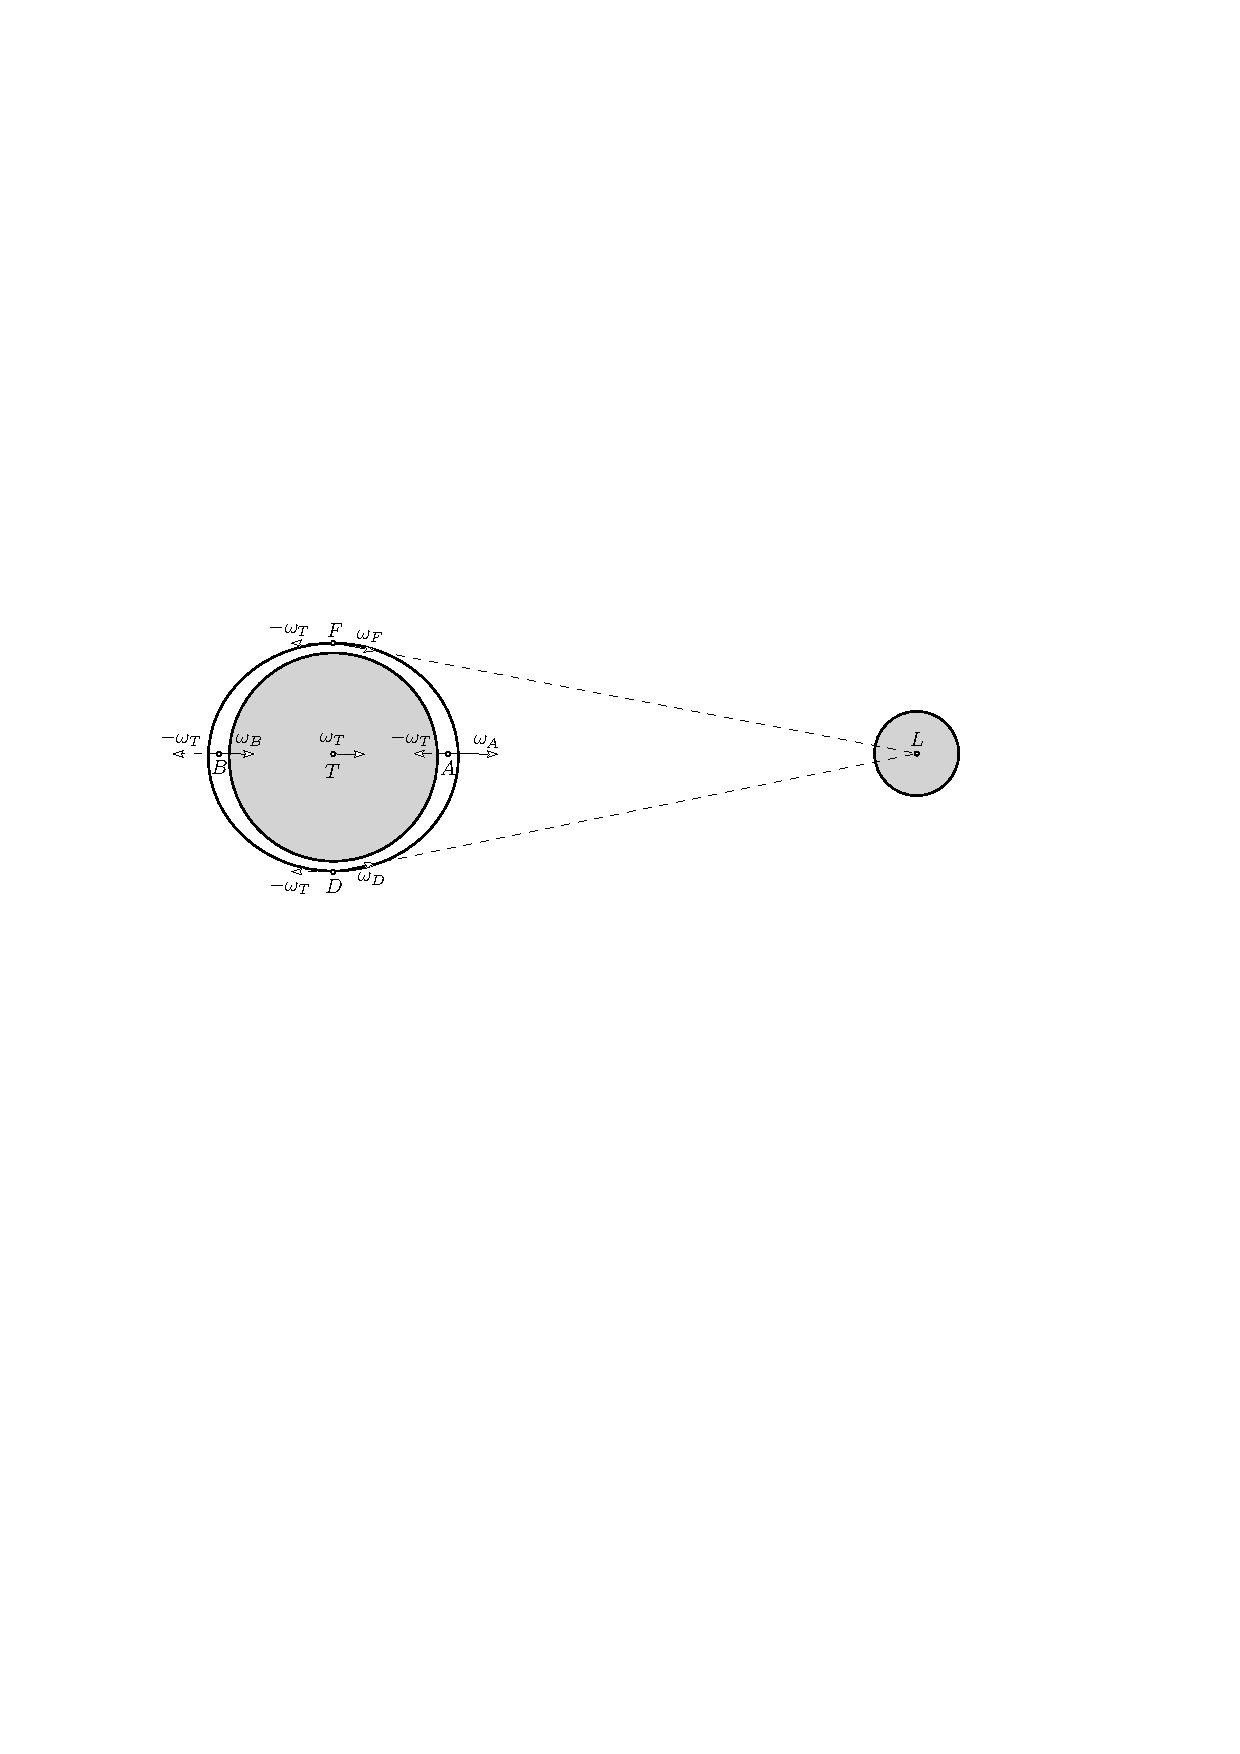
\includegraphics[width = 0.85\textwidth]{Ebb_flow}
\caption{К объяснению приливных сил}\label{Ebb_flow}
\end{figure}


\subsection{Солнечные и лунные затмения. Сарос}
\subsubsection{Полное солнечное затмение}
Диаметр тени спутника при полном центральном затмении (когда центры трёх тел лежат на одной прямой), с большой точностью равен: \begin{equation}
d_\text{тени} = 2 \frac{R_{\moon}(a - R_\oplus) - R_\odot \left( a - R_\oplus \right)}{a - a_{\moon}},
\end{equation}
где $R_{\moon}$~--- радиус Луны, 
$R_\oplus$~--- радиус Земли, 
$R_\odot$~--- радиус Солнца, 
$a$~--- расстояние от Земли до Солнца, 
$a_{\moon}$ --- расстояние от Земли до Луны.

Среднее значение  этой величины около 200 км, максимальное около 215 км. При нецентральном затмении максимальный диаметр тени Луны на поверхности Земли может достигать 270~км (Рис.\,\ref{fig:eclipses-full-solar-eslipse}).

\begin{figure}[h!]
\centering
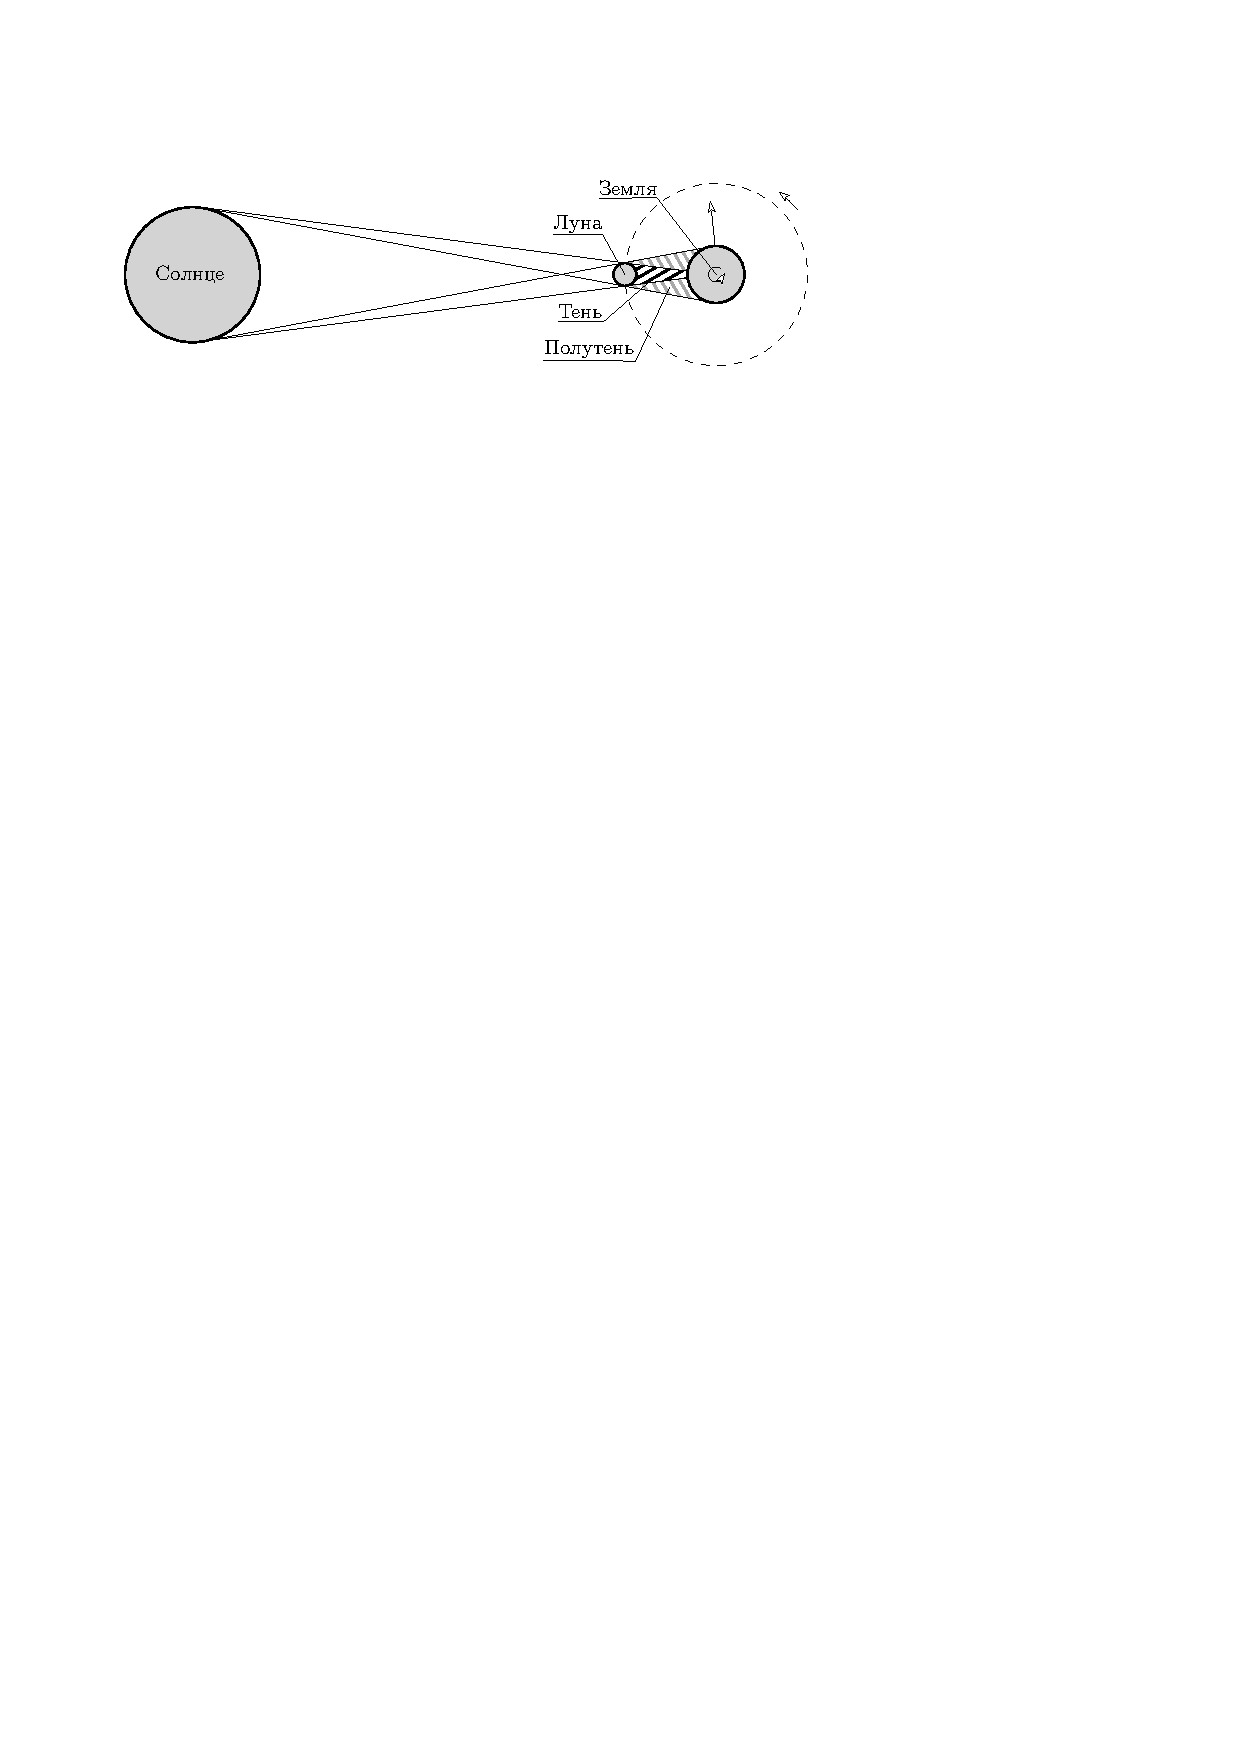
\includegraphics[width = .8\textwidth]{full_eclipse}
\caption{Полное солнечное затмение}
\label{fig:eclipses-full-solar-eslipse}
\end{figure}

\subsubsection{Кольцеобразное солнечное затмение}При кольцеобразном солнечном затмении Луна относительно Земли расположена так, что конус её тени не достаёт до поверхности планеты, и вокруг Луны можно наблюдать яркое кольцо незакрытой части солнечного диска (Рис.~\ref{fig:eclipses-circle-solar-eslipse}).
\begin{figure}[h!]
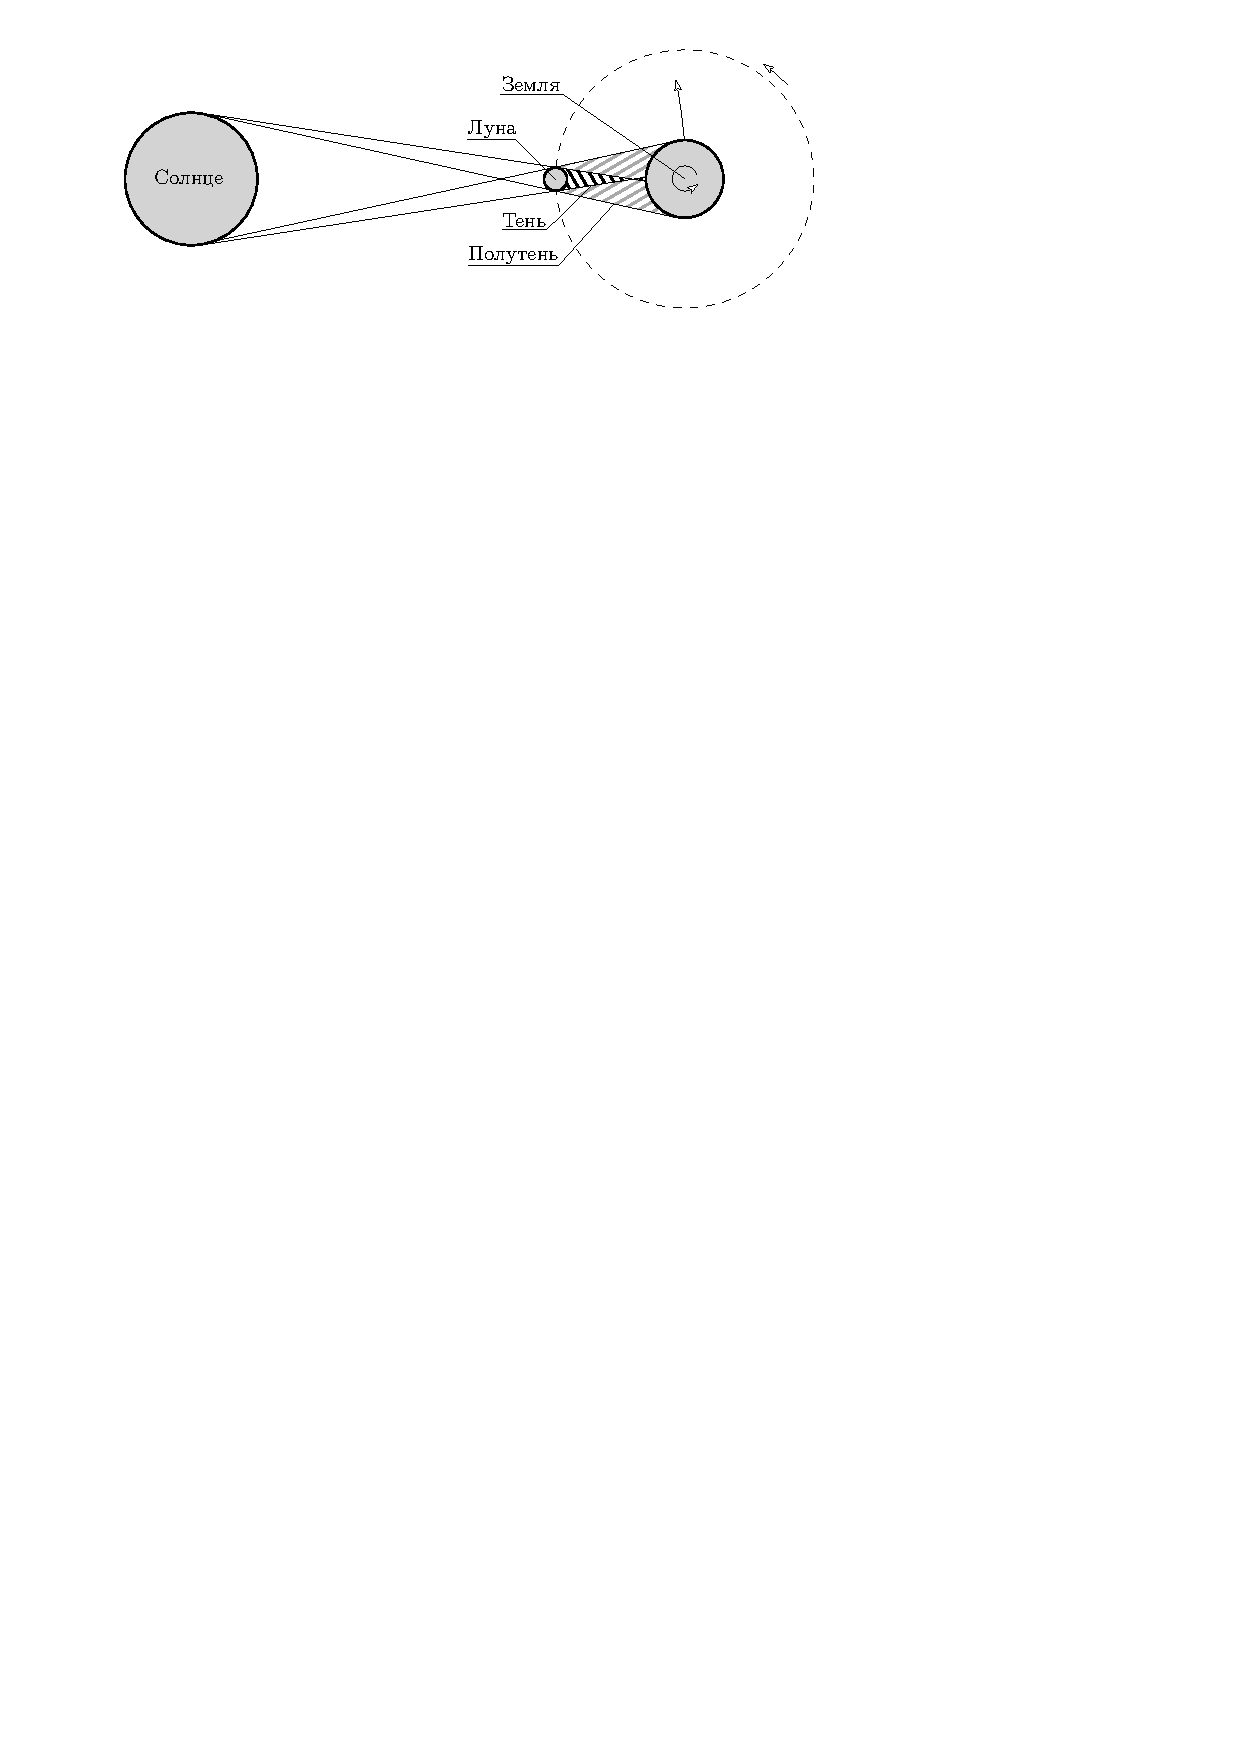
\includegraphics[width = 0.95\textwidth]{partly-eclipse}
\caption{Кольцеобразное солнечное затмение}
\label{fig:eclipses-circle-solar-eslipse}
\end{figure}

\subsubsection{Лунное затмение}

Лунное затмение в отличие от солнечного, видно со всего ночного полушария. Диаметр земной тени на расстоянии Луны превышает размер последней примерно в 2.5-3 раза (Рис.\,\ref{fig:moon-eclipse-scheme}).

\term{Синодический месяц} --- промежуток времени между одинаковыми фазами Луны. Он равен 29.53 суток.

\term{Драконический месяц} --- промежуток времени между двумя последовательными прохождениями Луны через один и тот же узел орбиты. Драконический месяц равен 27.21 суток.

\term{Сарос}~--- промежуток  времени, по прошествии которого солнечные и 
лунные затмения повторяются в прежнем порядке. Сарос составляет ровно 242 драконических месяца или 223 синодических месяца. Таким образом, его продолжительность примерно 18 лет 11 дней 8 часов.

\begin{figure}[h!]
\centering
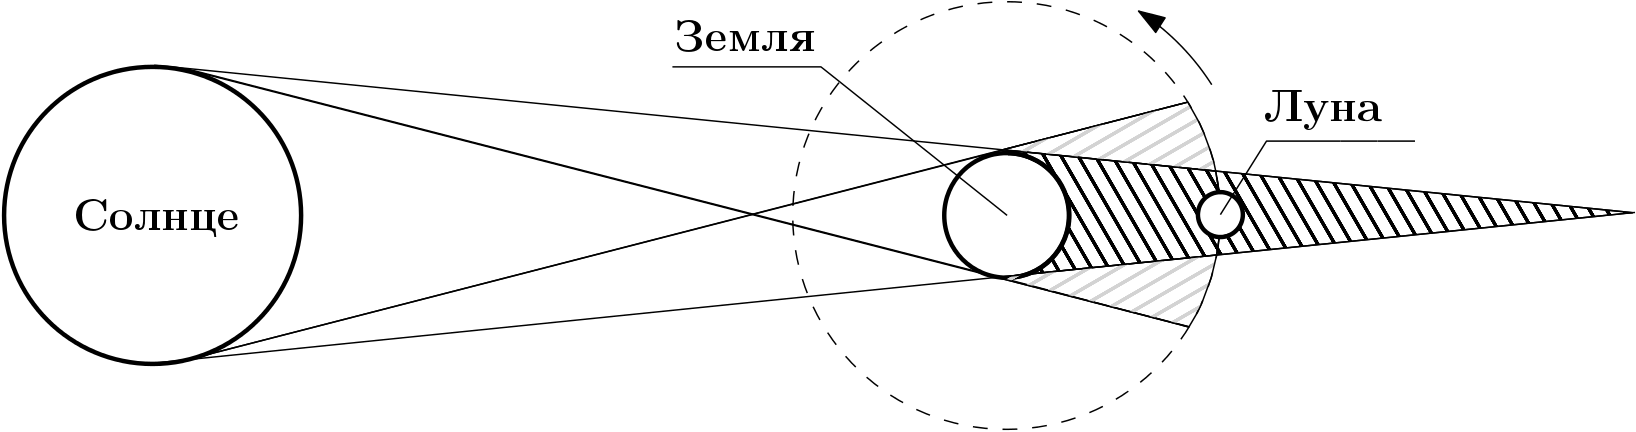
\includegraphics[scale=0.27]{moon-eclipse}
\caption{Схема лунного затмения}
\label{fig:moon-eclipse-scheme}
\end{figure}

\subsubsection{Фаза затмения}
Важной характеристикой любого затмения является его фаза. \term{Фаза затмения}~--- отношение закрытой части диаметра затмеваемого тела, проходящей через центр затмевающего тела, к полному диаметру затмеваемого тела. Для полного затмения эта величина рассчитывается немного иначе. Для Луны затмевающим <<телом>> является тень Земли. Фазу частного и полного затмения можно вычислить по следующим формулам (Рис.\,\ref{fig:part-eclipses-scheme}):\begin{equation}
\Phi_{\text{част}} = \frac{x}{D}, \quad \quad \quad \Phi_{\text{полн}} = 1 + \frac{d}{D},
\end{equation}
где $D$~--- диаметр затмеваемого тела.
\begin{figure}[h!]
\centering
\includegraphics[width = 0.3\textwidth]{phases}
\includegraphics[width = 0.3\textwidth]{phases-2}
\caption{Частное и полное затмение}
\label{fig:part-eclipses-scheme}
\end{figure}

Иногда вводят такое понятие, как \term{площадная фаза затмения}, т.е. отношение площади закрытой части диска затмеваемого диска к полной площади его диска. Чаще всего  площадную фазу используют применительно к двойным звёздам, когда считают падение блеска при затмении одной звезды другой.

\subsection{Конфигурации планет}
\term{Внутренними планетами} называются планеты, большая полуось орбиты 
$a$ которых меньше большой полуоси орбиты Земли $a_\oplus$. Отсюда следует, что для наблюдателя на Земле \imp{внутренними} планетами являются лишь Венера и Меркурий, остальные относятся к \imp{внешним}. Для таких планет выделяют три основные конфигурации: \imp{верхнее соединение}, \imp{нижнее соединение} и \imp{максимальная элонгация}. Различают две максимальные элонгации~--- \term{западную} и \term{восточную}, когда планета наблюдается к западу и к востоку от Солнца соответственно.

Внутренняя планета находится в \term{верхнем соединении}, когда Земля, Солнце и планета лежат на одной прямой, при этом планета и Земля располагаются по разные стороны от Солнца. Если пренебречь наклоном орбит планет к плоскости эклиптики, то для наблюдателя на Земле планета находится точно за Солнцем.

\begin{minipage}{0.36\tw}
\term{Нижнее соединение} внутренней планеты происходит когда Земля, Солнце и планета, также как и в случае верхнего соединения, располагаются на одной прямой, но для нижнего соединения планета должна находиться между Солнцем и Землей. Если бы орбиты всех планет лежали в одной плоскости, тогда в момент каждого нижнего соединения внутренней планеты наблюдалось бы ее прохождение по диску Солнца для наблюдателя на внешней планете.
\end{minipage}
\begin{minipage}{0.63\tw}
	\centering
	\vspace{-1pc}
	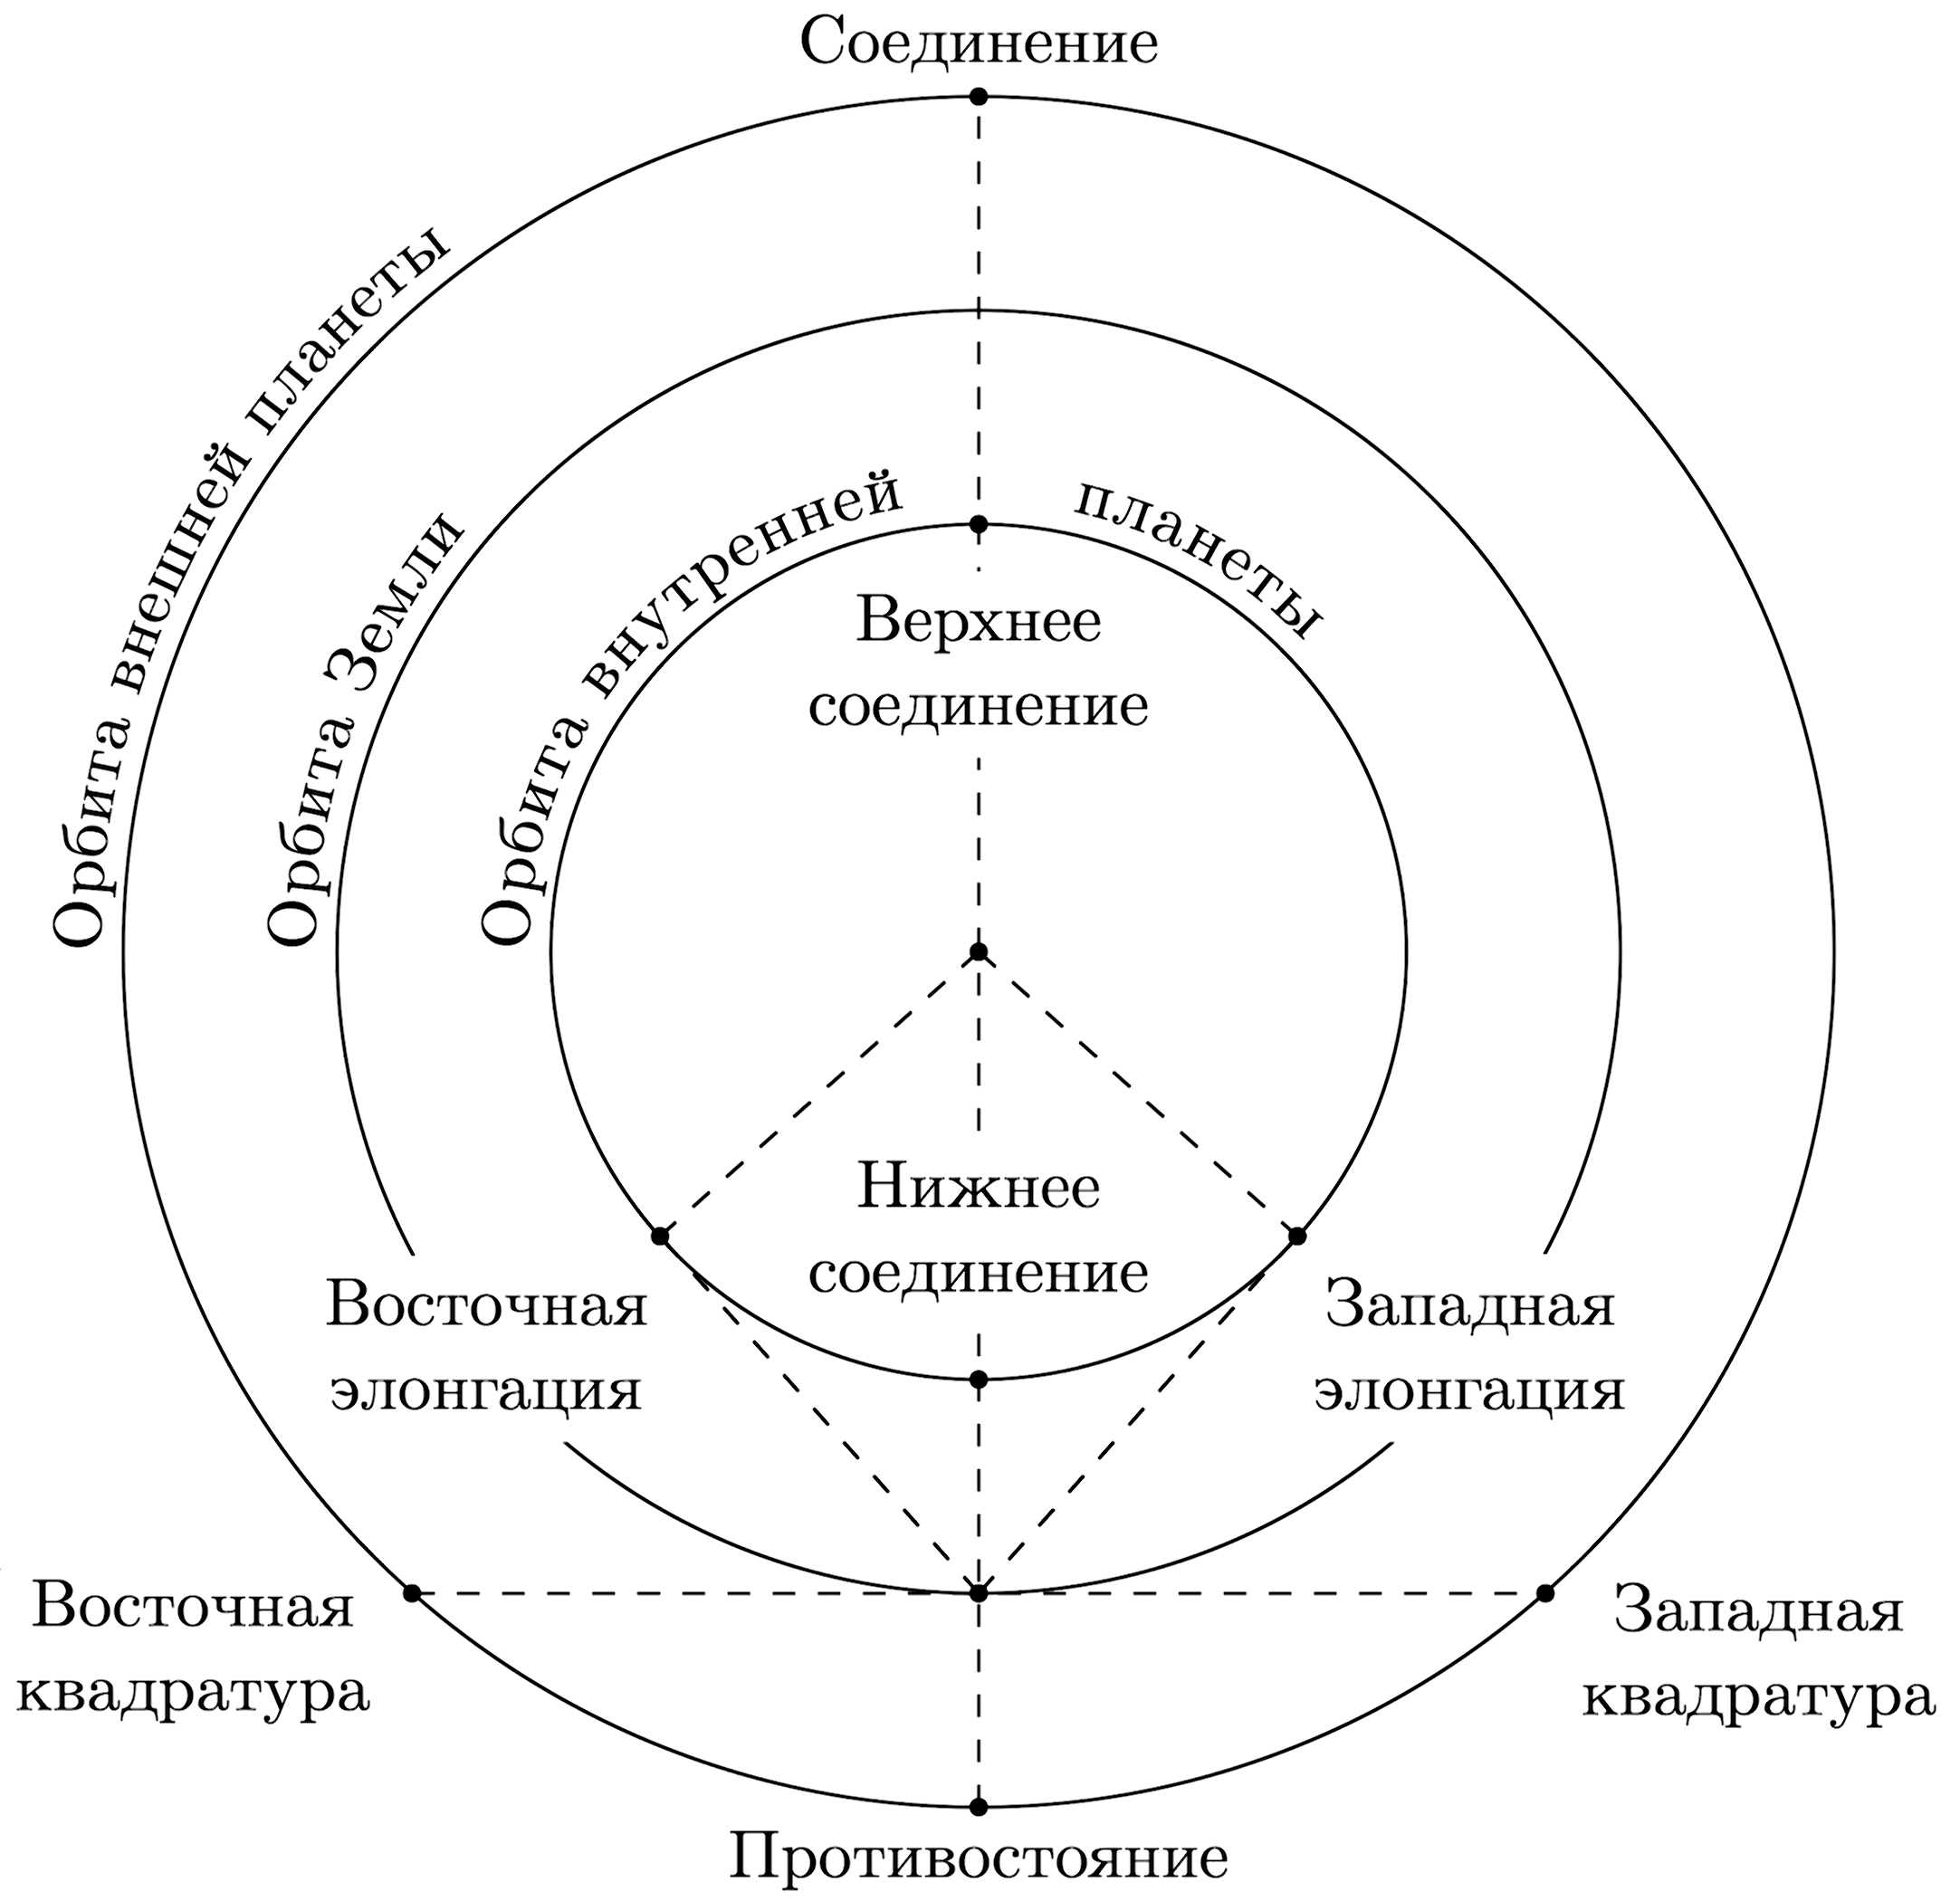
\includegraphics[width=\tw]{planet-config}
%\scriptsize
%\begin{tikzpicture}
%\fill [draw=black, fill=none,
%         postaction={decorate,decoration={raise=3pt,text along path, 
%           text={Орбита Земли}}}
%]
%  (-2.5, 0) arc (180:-180:2.5cm and 2.5cm);
%
%\fill [draw=black, fill=none,
%         postaction={decorate,decoration={raise=3pt,text along path,
%           text={Орбита внутренней~~~~~~~планеты}}}
%           ]
%  (-1.5, 0) arc (180:-180:1.5cm and 1.5cm);
%
%\fill [draw=black, fill=none,
%         postaction={decorate,decoration={raise=3pt,text along path,
%           text={Орбита внешней планеты}}}
%           ]
%  (-3.5, 0) arc (180:-180:3.5cm and 3.5cm);
%  
%\draw [dashed] (-2.65, -3) -- (2.65, -3);
%\draw [dashed] (0, -4) -- (0, 4);
%\draw [dashed] (0, -3) -- (-1.49, -1.33);
%\draw [dashed] (0, 0) -- (-1.49, -1.33);
%\draw [dashed] (0, -3) -- (1.49, -1.33);
%\draw [dashed] (0, 0) -- (1.49, -1.33);
%
%\filldraw [black] (0, 0) circle (1pt);
%\filldraw [black] (-1.49, -1.33) circle (1pt);
%\filldraw [black] (1.49, -1.33) circle (1pt);
%\filldraw [black] (2.65, -3) circle (1pt);
%\filldraw [black] (-2.65, -3) circle (1pt);
%\filldraw [black] (0, -3) circle (1pt);
%\filldraw [black] (0, 2) circle (1pt);
%\filldraw [black] (0, 4) circle (1pt);
%\filldraw [black] (0, -2) circle (1pt);
%\filldraw [black] (0, -4) circle (1pt);
%
%\draw (-3.7, -3.7) -- (-3.7, -3.7) node  [above,align=center,midway]{Западная\\квадратура};
%    
%\draw (3.7, -3.7) -- (3.7, -3.7) node  [above,align=center,midway]{Восточная\\квадратура};
%    
%\draw (0, -4.5) -- (0, -4.5) node  [above,align=center,midway]{Противостояние};
%
%\draw (0, 4) -- (0, 4) node  [above,align=center,midway]{Соединение};
%
%\draw (0, 0.9) -- (0, 0.9) node  [fill=white,above,align=center,midway]{Верхнее\\соединение};
%
%\draw (0, -1.75) -- (0, -1.75) node  [fill=white,above,align=center,midway]{Нижнее\\соединение};
%
%\draw (0.6, -3.4) -- (0.6, -3.4) node  [above,align=center,midway]{\ttfamily Земля};
%
%\draw (0.7, -0.2) -- (0.7, -0.2) node  [above,align=center,midway]{\ttfamily Солнце};
%
%\draw (2.3, -2.3) -- (2.3, -2.3) node  [fill=white,above,align=center,midway]{Западная\\элонгация};
%
%\draw (-2.3, -2.3) -- (-2.3, -2.3) node  [fill=white,above,align=center,midway]{Восточная\\элонгация};
%
%\end{tikzpicture}
	\captionof{figure}{Конфигурации планет}
\end{minipage}\\

\term{Элонгацией} планеты называется угол Солнце -- Земля -- планета, отсюда очевидно, что \imp{максимальная элонгация} внутренней планеты наблюдается в момент, когда прямая Земля -- планета является касательной к орбите планеты, то есть угол Солнце -- планета -- Земля является прямым.

\term{Внешними планетами} называются планеты, большая полуось орбиты $a$ которых больше большой полуоси орбиты Земли $a_\oplus$. Для таких планет также существуют три основные конфигурации: \imp{соединение}, \imp{противостояние} и \imp{квадратура}. Квадратура бывает \term{западная} и \term{восточная}, в какой именно квадратуре находится внешняя планета определяется аналогично максимальной элонгации.

\term{Соединение} внешней планеты, подобно верхнему соединению внутренней планеты, наблюдается в момент, когда Солнце, Земля и планета находятся на одной прямой, при этом Солнце находится между планетой и Землей. В этот момент для наблюдателя на внешней планете Земля, являясь нижней планетой, наблюдается в верхнем соединении.

Аналогично, когда планета, Солнце и Земля располагаются на одной прямой, но Солнце и планета лежат по разные стороны от Земли, считается, что внешняя планета находится в \term{противостоянии}. Земля же находится в нижнем соединении для наблюдателя на внешней планете, наблюдаемой в противостоянии.

\term{Квадратурой} называется конфигурация, когда угол между направлениями на планету и Солнце (угол {\slshape Солнце -- Земля -- планета}) является прямым. Стоит заметить, что для наблюдателя на планете Земля будет наблюдаться в максимальной элонгации, причем если планета с Земли наблюдалась в восточной квадратуре, тогда Земля будет в западной максимальной элонгации и наоборот.


\subsection{Синодический период}

\term{Синодический период} (период смены фаз)~--- время, прошедшее между двумя последовательными одноимёнными конфигурациями одного тела при наблюдении с другого.

\imp{Относительная угловая скорость} планет равна 
разности скоростей углового перемещения одной планеты ($2\pi/T_1$) и другой ($2\pi/T_2 $) по орбите. Из определения относительной угловой скорости вытекает общая формула для продолжительности синодического периода: 
\begin{equation}
\frac1S=\left| \frac1T_1-\frac1T_2 \right|.
\end{equation}
Для внешних и внутренних планет соответственно выражения принимает следующий вид: 
\begin{equation} \frac{1}{S} = \frac{1}{T_\oplus} - \frac{1}{T_\text{пл}} \quad \text{и} \quad \frac{1}{S} = \frac{1}{T_\text{пл}} - \frac{1}{T_\oplus},
\end{equation}
где $S$~--- синодический период, $T_\text{пл}$~--- сидерический период планеты, $T_\oplus$~--- сидерический период обращения Земли.

В случае, если тела обращаются в противоположные стороны, то связь 
их синодического периода с сидерическими очевидным образом принимает вид:
\begin{equation}
\frac1S=\frac1T_1+\frac1T_2.
\end{equation}
\subsection{Фазы планет и спутников}

\term{Фаза} планеты (спутника)~--- отношение площади освещённой  части видимого диска ко всей его площади.
Фаза рассчитывается по формуле
\begin{equation}
\Phi = \frac{1 + \cos \phi}{2} = \cos^2 \frac{\phi}{2},
\end{equation}
\begin{minipage}{0.67\tw}
где $\phi$~--- \term{фазовый угол} --- угол между лучом света, падающим от Солнца на планету, и лучом, отразившимся от неё в сторону наблюдателя (см.~Рис.\,\ref{fig:phase-angel-scheme}). Фаза объекта может принимать значения от 0 до 1.

Видимая границы между освещенной и неосвещенной частями поверхности объекта называется \term{терминатором}. В зоне терминатора для наблюдателя на объекте источник пересекает горизонт.
\end{minipage}
\hfill
\begin{minipage}{0.31\tw}
	\hfill
	\vspace{-.5pc}
	\includegraphics[width = \tw]{phase-angle}
	\captionof{figure}{Фазовый угол}
	\label{fig:phase-angel-scheme}
\end{minipage}


\subsection{Прецессия}
\begin{wrapfigure}[15]{l}{0.41\tw}
	\vspace{-1pc}
	\centering
	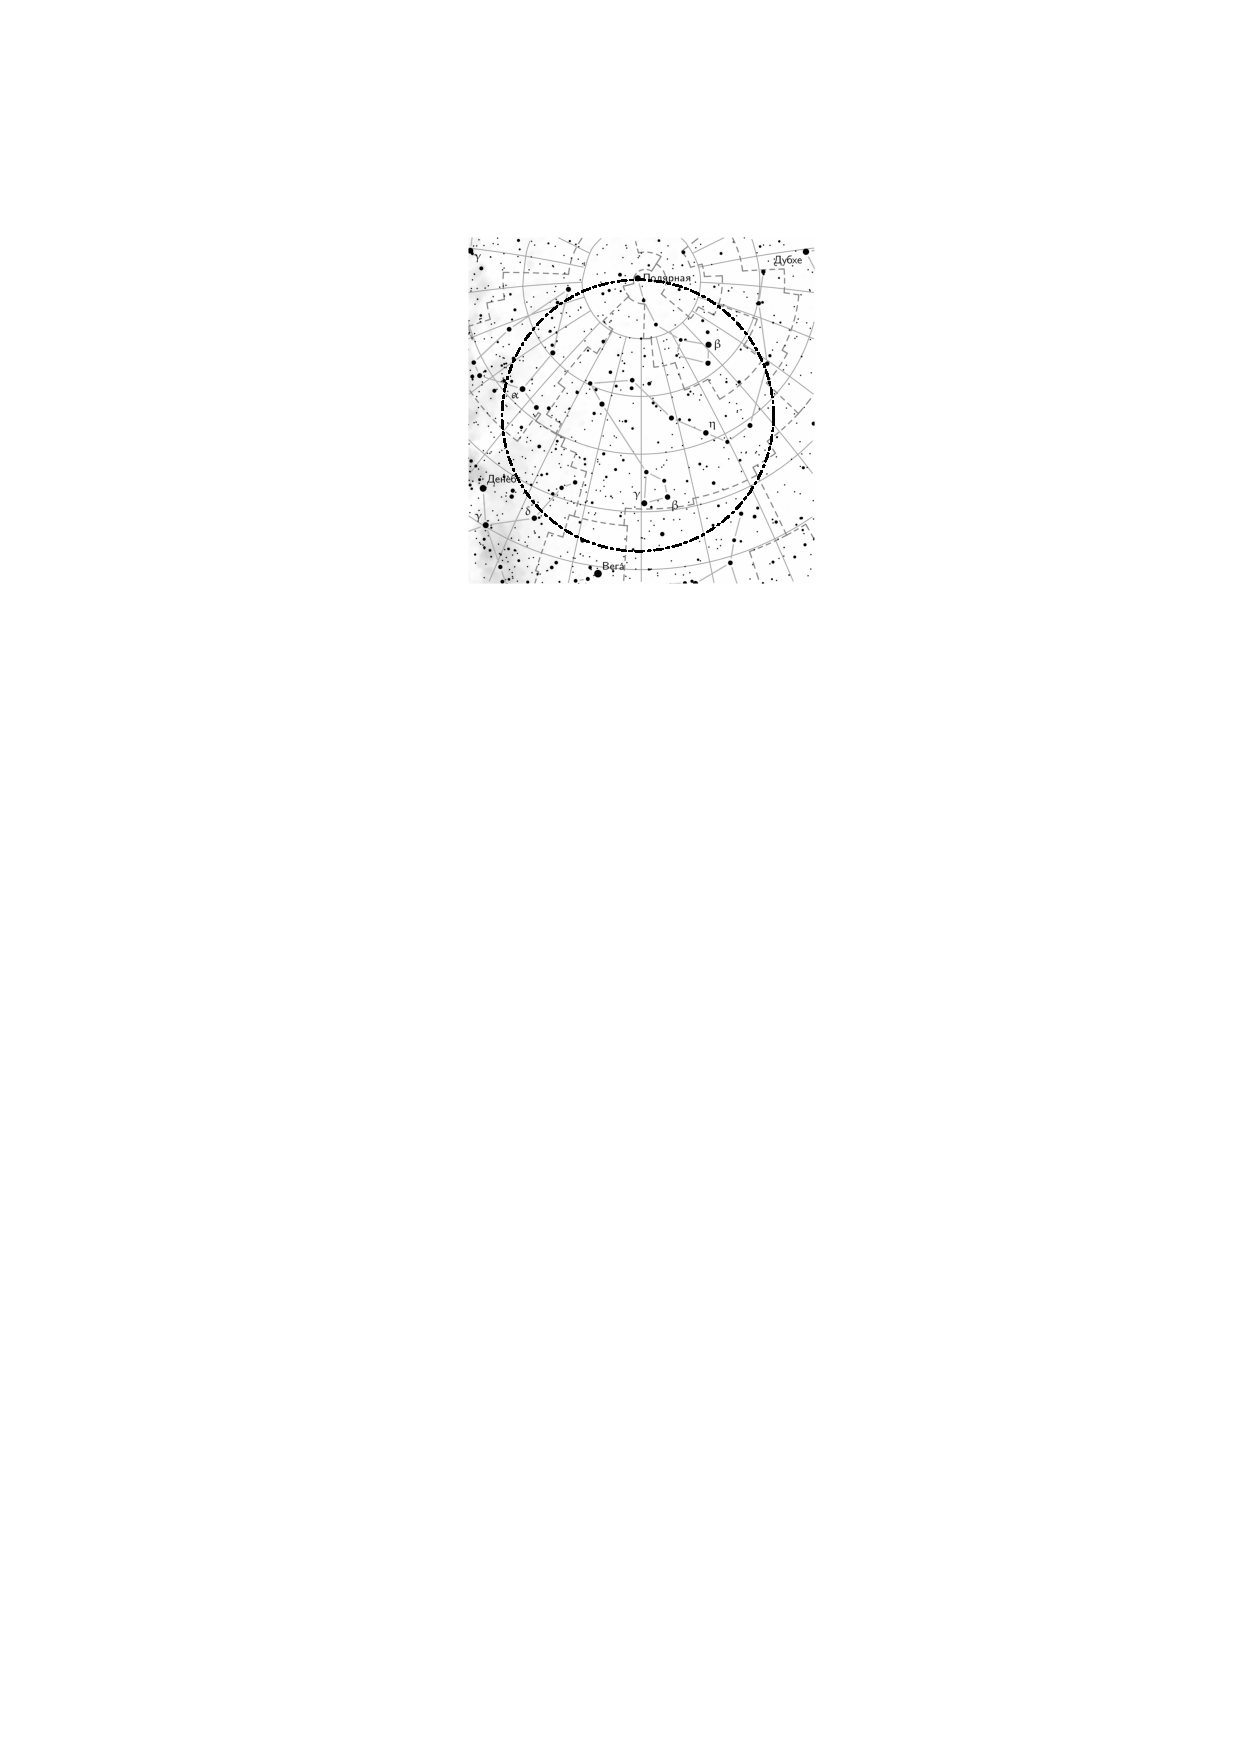
\includegraphics[width = .42\tw]{precession_bw}
	\caption{Прецессионное движение северного полюса мира}
	\label{fig:precession-path}
\end{wrapfigure}
Под действием возмущающих сил ось вращения Земли совершает прецессионное движение: описывает вокруг оси эклиптики конус с углом раствора $23.5^\circ$ с периодом около  25\,765~лет. Из-за этого меняется положение полюс мира. Например, сейчас полюс мира практически совпадает с Полярной звездой ($\alpha$\,UMi), а 15\,000~лет назад роль полярной звезды играла Вега ($\alpha$\,Lyr). Если считать, что величина прецессии постоянна, то полюсы мира описывают вокруг полюсов эклиптики малые круги с радиусом $23.5^\circ$. В~действительности~же величина прецессии меняется, поэтому путь полюсов мира представляет собой не~окружность, а~спираль.

Поворот оси Земли имеет различные последствия. Во-первых, меняется продолжительность тропического года, он становится примерно на $20$~минут короче звёздного. Во-вторых, из-за прецессии меняется вид звёздного неба, хоть и происходит это очень медленно (см.~Рис.\,\ref{fig:precession-path}).
\section{Конические сечения}
\subsection{Эллипс}
{\bfseries \term{Эллипс}} --- плоская замкнутая кривая, сумма 
расстояний от любой точки которой до двух фиксированных 
точек, называемых фокусами, постоянна и равна 
удвоенной большой полуоси эллипса.
\begin{equation}|F_1 M|+|F_2M|=const=2a
\end{equation}

Главные отрезки эллипса: \term{большая полуось} 
($a$), \term{малая полуось} ($b$), \term{ 
фокусное расстояние} ($c$). Они связаны следующим 
соотношением: $b^2+c^2=a^2$, что несложно вывести из 
определения эллипса.

\term{Эксцентриситет} ($e$) --- числовая 
характеристика, показывающая степень отклонения от 
окружности. Для эллипса $e$ лежит в интервале $(0, \, 1)$ и
определяется следующей формулой:\begin{equation}
p=\frac{b^2}{a}=a(1-e^2)=b\sqrt{1-e^2}
\end{equation}

\begin{figure}[h!]
\centering
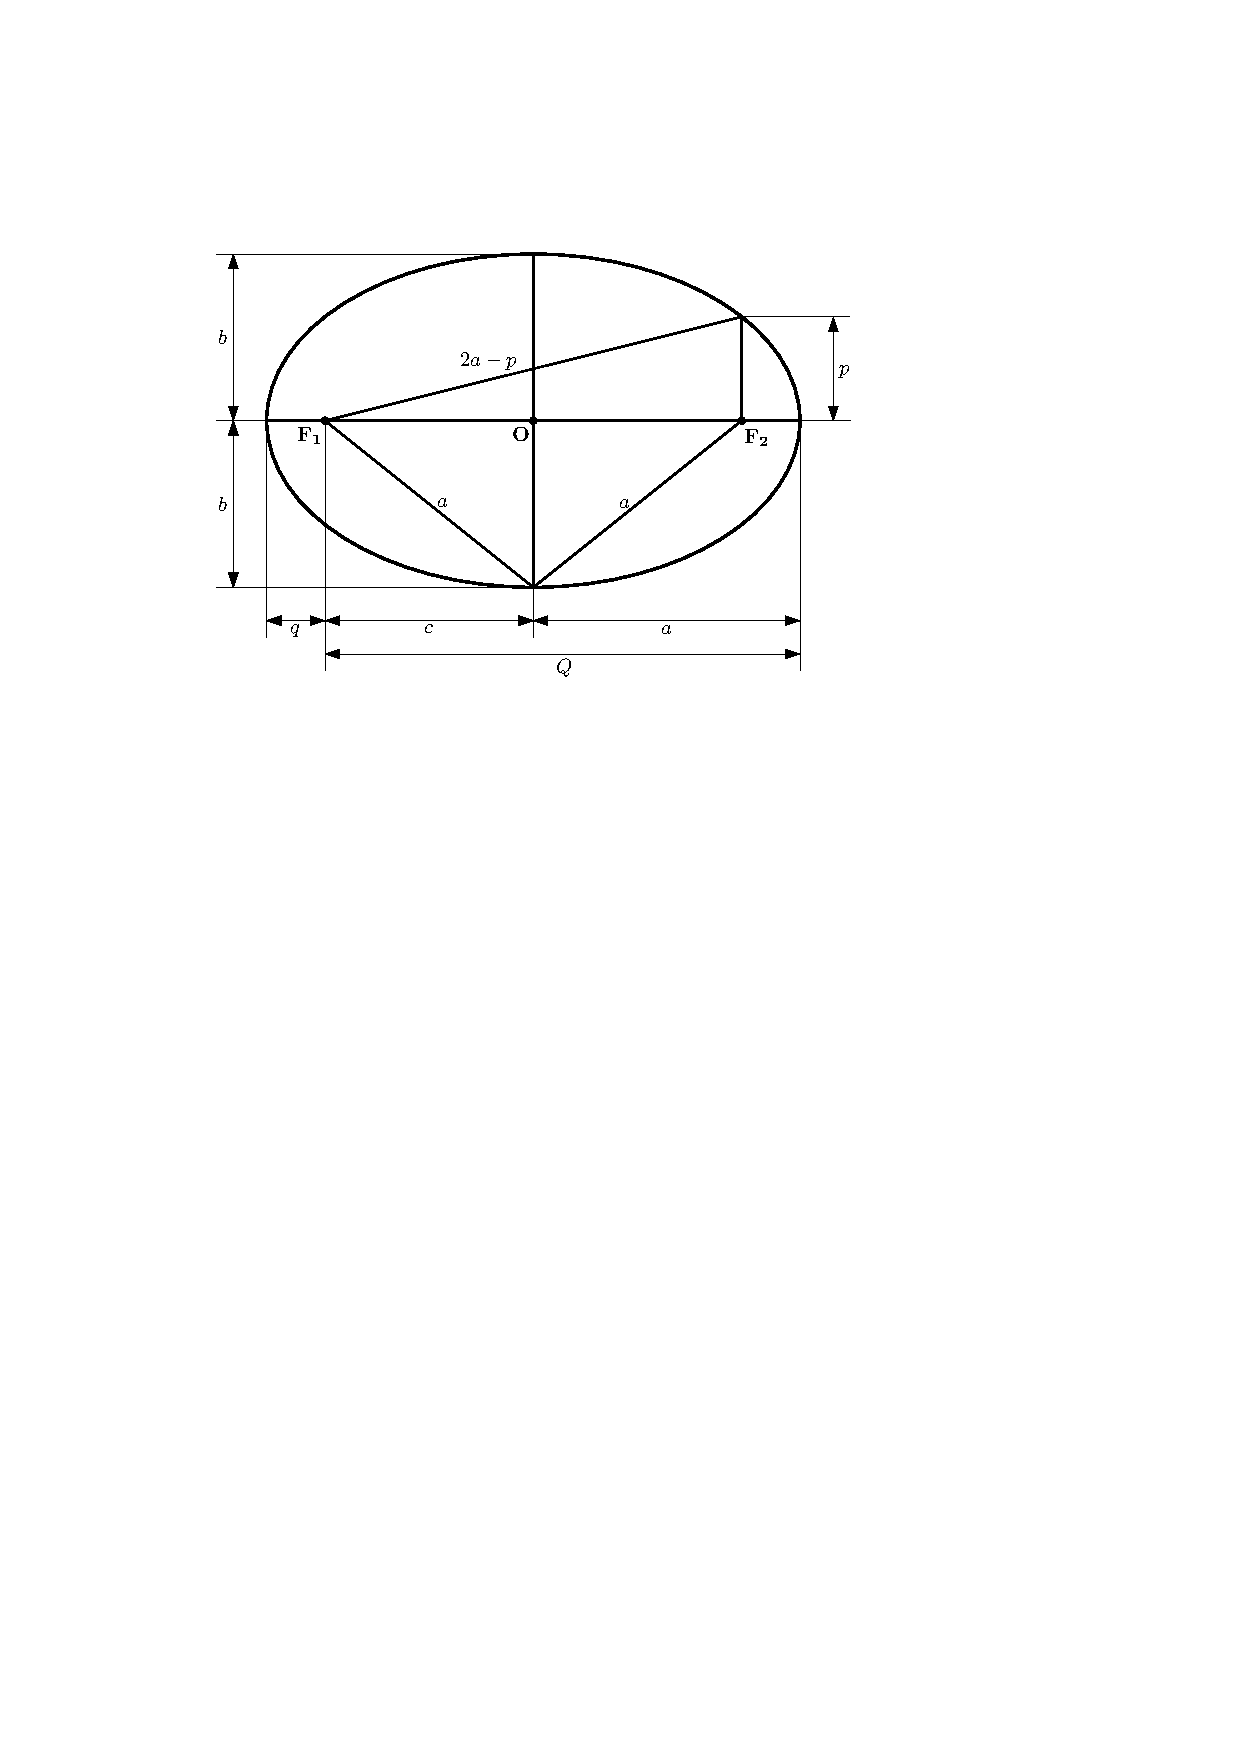
\includegraphics[width = 0.8\textwidth]{Ellips}
\caption{Эллипс}
\end{figure}

\term{Апоцентр} --- наиболее удаленная точка
от заданного фокуса точка эллипса. Из определения эллипса
вытекает соотношение для расстояния от фокуса до 
апоцентра ($Q$):\begin{equation}
Q = a (1 + e)
\end{equation}

\term{Перицентр} --- ближайшая точка
точка эллипса к заданному фокусу . Из определения эллипса
вытекает соотношение для расстояния от фокуса до 
перицетра ($q$):\begin{equation}
q = a (1 - e)
\end{equation}

\term{Фокальный параметр} ($p$) --- длина перпендикуляра,
проведенного из фокуса до точки пересечения с эллипсом.
Из теоремы Пифагора и определения эллипса следует 
нижеприведенная формула для расчета его длины. 
\begin{equation}
p = a(1 - e^2)
\end{equation}

\term{Площадь эллипса} ($S$) --- площадь части 
плоскости, ограниченной эллипсом. Выражение для площади 
эллипса можно находить интегрированием по полярному углу, 
используя уравнение эллипса в полярных координатах или 
пользуясь свойством аффинного преобразования сжатия из 
выражения площади окружности с радиусом $a$:
\begin{equation}
S=\pi ab
\end{equation}

%Радиус кривизны дуги эллипса в зависимости от расстояния 
%$x$ от фокуса:
%\begin{equation}
%R=\frac{(2ax-x^2)^{3/2}}{ab}
%\end{equation}
%\begin{center}
%
\includegraphics[width = 0.3\textwidth]{rad-curv}
%\begin{figure}[!h]
%\caption{К вычислению радиуса кривизны эллипса}
%\end{figure}
%\end{center}

{\itshape Уравнение эллипса} в декартовых координатах 
представляет собой уравнение замкнутой кривой второго 
порядка, канонический вид которого имеет следующий вид:
\begin{equation}
\frac{x^2}{a^2}+\frac{y^2}{b^2}=1
\end{equation}

Его можно представить параметрическом виде:\begin{equation}
\left\{\begin{aligned}[lcl]
&x=a\cos t;\\
&y=b\sin t,\\
\end{aligned}
\right.
\end{equation}
где параметр $t \in [0, \, 2\pi)$.

В полярных координатах уравнение принимает следующий вид:
\begin{equation}
r=\frac{p}{1\pm e\cos\phi},
\end{equation} 
где $\varphi$ --- \term{истинная аномалия} --- угол 
{\slshape перицентр -- фокус -- заданная точка}, 
отсчитываемый в сторону движения по эллипсу. При 
положительном знаке перед $e$ второй фокус эллипса будет 
находится в точке $(0, \, 2c)$, а при отрицательном --- в 
точке $(\pi, \, 2c)$.\\

Кроме этого, эллипс обладает важным {\itshape оптическим 
свойством}, которе можно сформулировать так: свет от источника в одном из фокусов, 
	отражается эллипсом так, что отражённые лучи пересекаются 
	во втором фокусе или, что тоже самое, касательная к эллипсу в заданной точке образует с фокальными радиусами в данной точке равные острые углы.






 

\subsection{Парабола}

{\bfseries \term{Парабола}} --- геометрическое место точек, равноудалённых от данной прямой (называемой \term{директрисой} параболы) и данной точки (называемой \term{фокусом} параболы).

{\itshape Каноническое уравнение параболы} имеет следующий вид:
\begin{equation}
y^2=2px,
\end{equation}
где $p$ --- \term{фокальный параметр}, равный расстоянию между фокусом параболы и директрисой или удвоенному расстоянию между фокусом параболы и вершиной.

Парабола в полярной системе координат $(\rho,\varphi)$ с центром в фокусе и нулевым направлением вдоль оси параболы (от фокуса к вершине) может быть представлена в виде уравнения
\begin{equation}
\rho(1+\cos\varphi)=p
\end{equation}

Эксцентриситет параболы равен $e=1$.
Важно отметить, что парабола не имеет \term{большой} и \term{малой полуоси}.

\begin{figure}[h!]
\centering
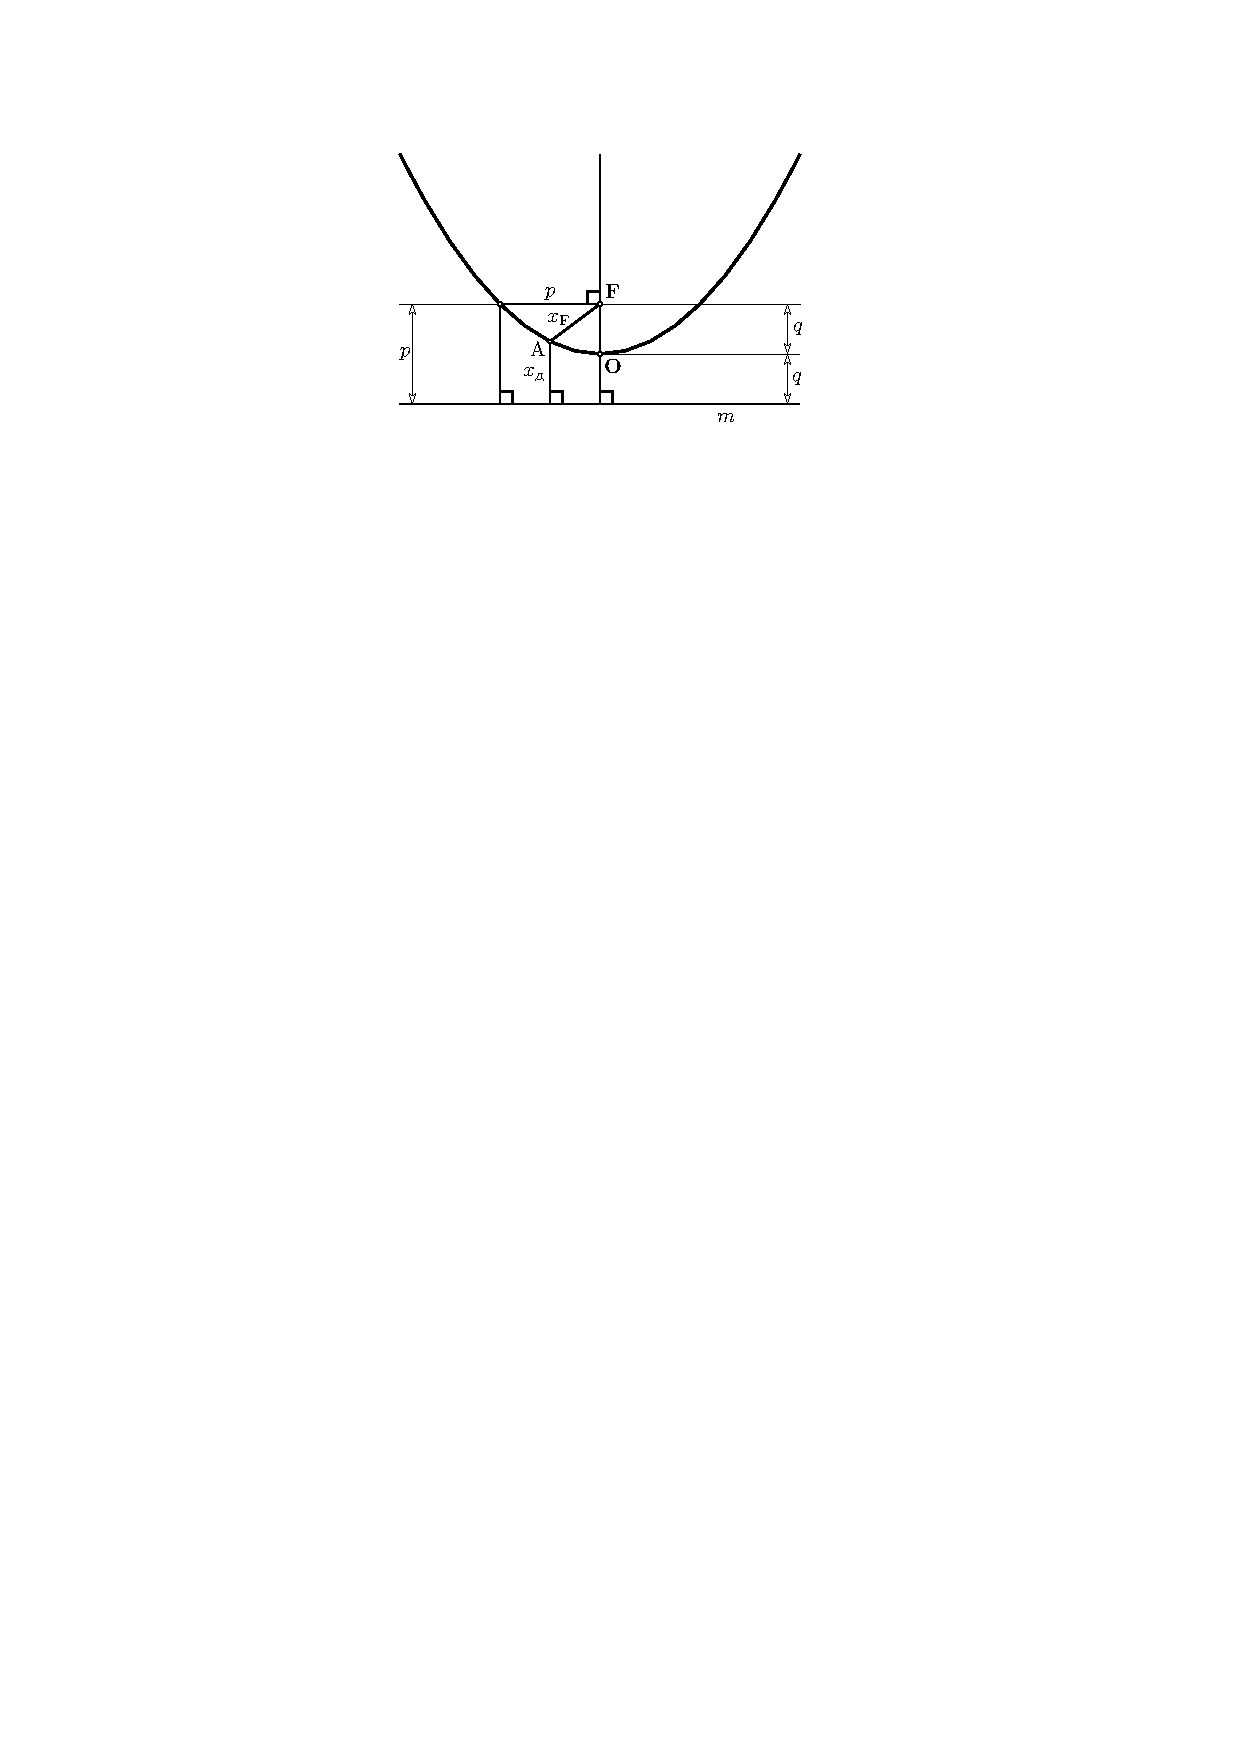
\includegraphics[width = 0.8\textwidth]{Parabola}
\caption{Парабола \label{pic:the-pic}}
\end{figure}

Как и все конические сечения, парабола обладает \textit{оптическим свойством}, которое формулируется следующим образом: пучок лучей, параллельных оси параболы, отражаясь в параболе, собирается в её фокусе. И наоборот, свет от источника, находящегося в фокусе, отражается параболой в пучок параллельных её оси лучей.


\subsection{Гипербола}
 
{\bfseries \term{Гипербола}} --- геометрическое место точек евклидовой плоскости, абсолютное значение разности расстояний от которых до двух выделенных точек $F_1$ и $F_2$, называемых фокусами, постоянно и равно удвоенной действительной полуоси гиперболы.
\begin{equation}
\bigl||F_1M|-|F_2M|\bigr|=2a
\end{equation}
\begin{figure}[h!]
\centering
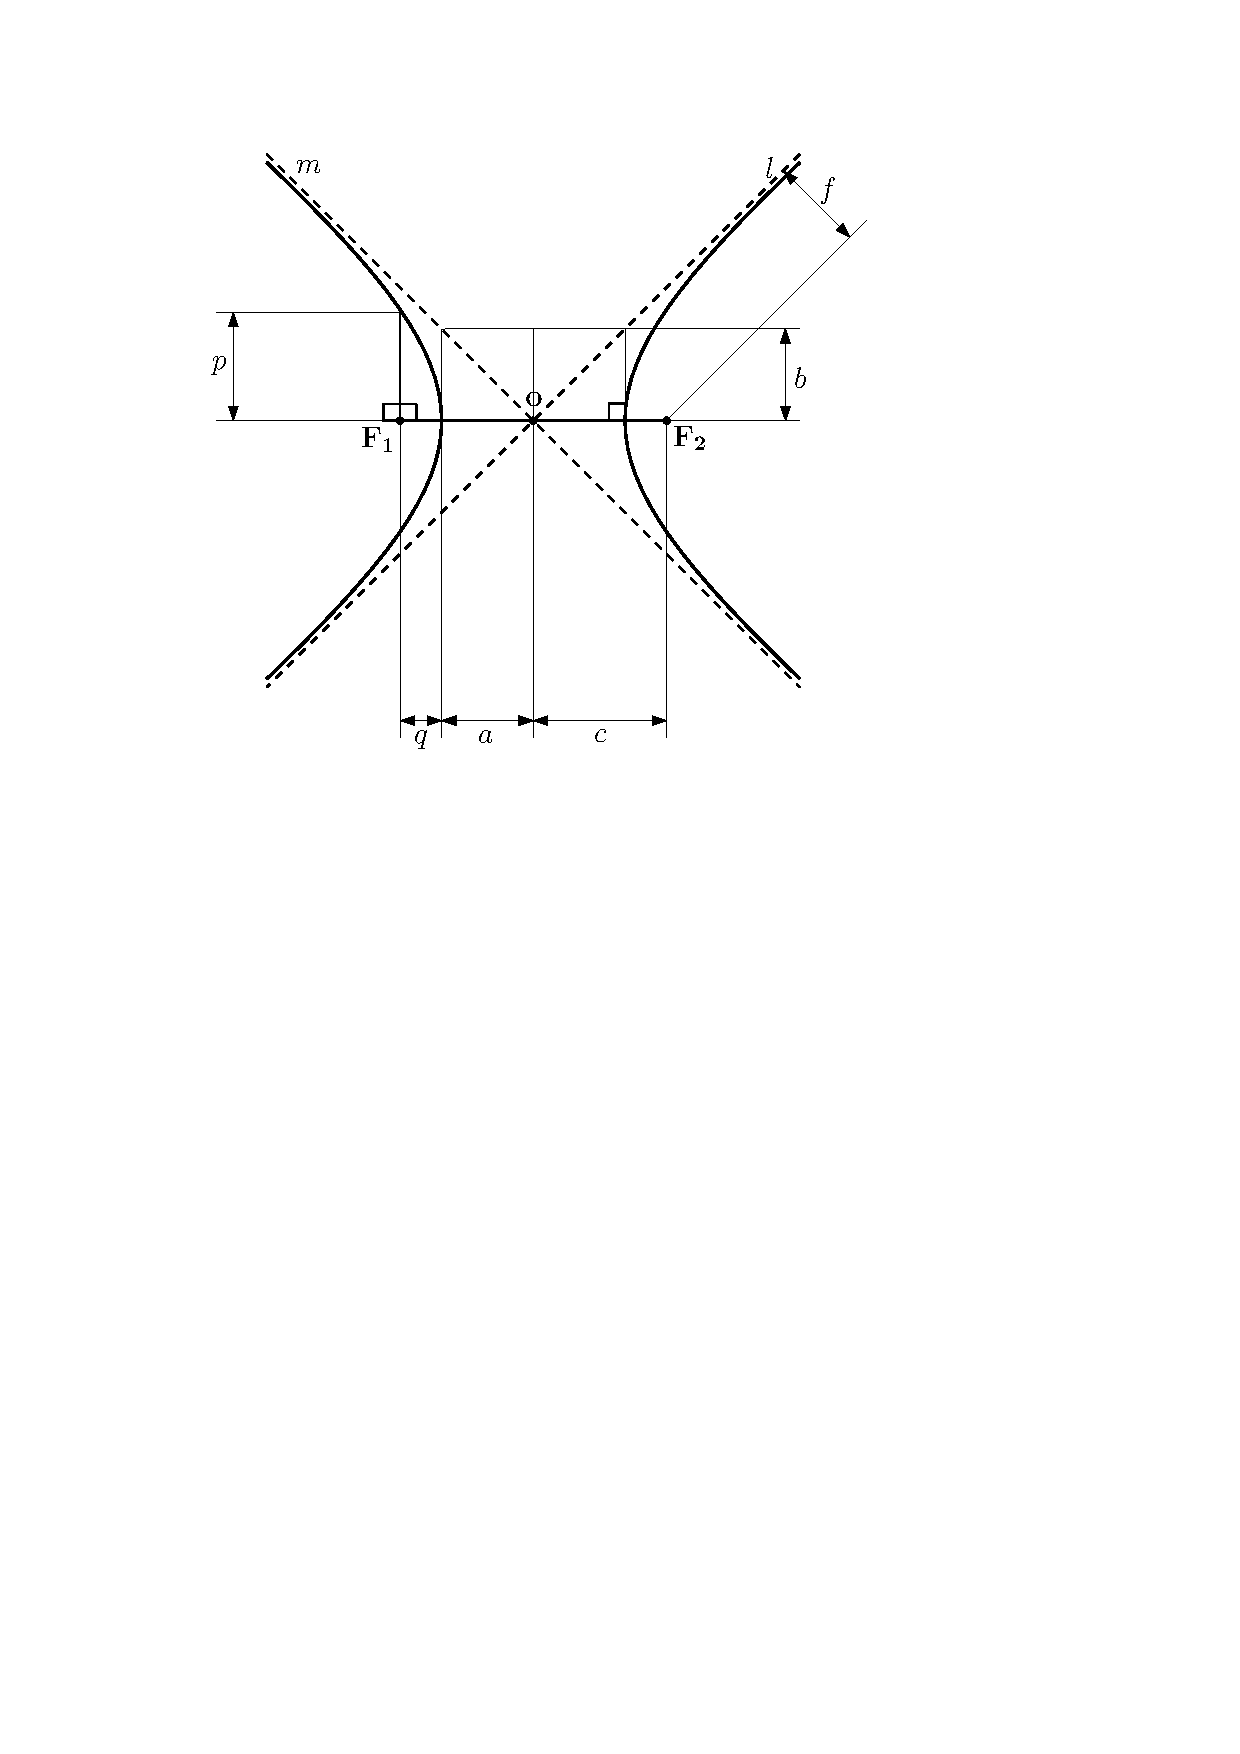
\includegraphics[width = 0.6\textwidth]{Hiperbola}
\caption{Гипербола \label{pic:the-pic}}
\end{figure}

Ближайшие друг к другу точки двух ветвей гиперболы называются \term{вершинами} гиперболы.

\term{Большая} или \term{действительная полуось} ($a$) гиперболы --- расстояние от центра гиперболы до одной из вершин.

\term{Действительная} или \term{поперечная} ось ---  прямая, содержащая большую ось гиперболы

\term{Фокальное расстояние} ($c$) ---  расстояние от центра гиперболы до одного из фокусов.

\term{Эксцентриситетом} гиперболы ($e$), как и  эллипса, является отношение фокального расстояния к большой полуоси, так как большая полуось гиперболы всегда больше ее фокального расстояния, эксцентриситет гиперболы $e > 1$ и может быть найдет из определения:\begin{equation}
e=\frac{c}{a}
\end{equation}

\term{Перицентрическое расстояние} ($q$) --- расстояние от фокуса до ближайшей вершины гиперболы.\begin{equation}
q=a(e-1)
\end{equation}

\term{Мнимая полуось} ($b$) --- длина перпендикуляра к оси абсцисс, восставленного из вершины до пересечения с асимптотой. Равна прицельному параметру.

\term{Мнимая} или \term{сопряжённая} ось --- прямая, перпендикулярная действительной оси и проходящая через её центр.

\term{Прицельный параметр} ($f$) --- расстояние от фокуса до асимптоты гиперболы.

\term{Фокальный параметр} ($p$) --- длина отрезка, перпендикулярного к действительной оси, проведённого от фокуса до гиперболы.
\begin{equation}
p=\frac{b^2}{a}
\end{equation}\\

{\itshape Каноническое уравнение гиперболы} в прямоугольных декартовых координатах записывается следующим образом:\begin{equation}
\frac{x^2}{a^2}-\frac{y^2}{b^2}=1
\end{equation}

В {\itshape полярных координатах уравнение} принимает следующий вид:\begin{equation}
r=\frac{p}{1-e\cos\varphi},
\end{equation}
причём полюс находится в фокусе гиперболы, а вершина гиперболы лежит на продолжении полярной оси.\\

{\itshape Уравнение двух асимптот} является уравнением пересекающихся прямых и принимает следующий вид:\begin{equation}
\frac{x}{a}\pm\frac{y}{b}=0
\end{equation}\\

Ниже представлены важные соотношения, справедливые для гиперболы:
\begin{equation}
c^2=a^2+b^2
\end{equation}\\

Также, как и любое коническое сечение, гипербола имеет своё {\itshape оптическое свойство}: свет от источника, находящегося в одном из фокусов гиперболы, отражается второй ветвью гиперболы таким образом, что продолжения отраженных лучей пересекаются во втором фокусе.

\section{Астрофизика}
\subsection{Чёрные дыры}
\term{Чёрная дыра}~(ЧД)~--- область пространства-времени с массой $M$, гравитационное притяжение которой настолько велико, что покинуть её не могут даже объекты, движущиеся со скоростью света $c$. Граница этой области называется \imp{горизонтом событий}, а её характерный размер~$R_G$~--- \imp{гравитационным радиусом}, для величины которого справедливо равенство
\begin{equation}
R_G = \frac{2 G M}{c^2}.
\end{equation}

Минимальная масса ЧД составляет около $2.5M_{\odot}$. А плотность ЧД определяется отношением ее массы~$M$ к~объему~$V$, следовательно
\begin{equation}
\rho = \frac{M}{V} = \frac{3c^6}{32\pi M^2G^3}.
\end{equation}

\term{Эффект излучения} (испарения) \term{Хокинга}~--- эффект, при котором гравитационное поле черной дыры поляризует вакуум, в результате чего возможно образование не только виртуальных, но и реальных пар частица~--античастица. Одна из частиц, оказавшаяся чуть ниже горизонта событий, падает внутрь чёрной дыры, а другая, оказавшаяся чуть выше горизонта, улетает, унося энергию (то есть часть массы) чёрной дыры. Для мощности излучения ЧД справедлива формула
\begin{equation}
L = \frac{h c^6}{30720 \pi^2 G^2 M^2},
\end{equation}
где $h$ --- постоянная Планка. Спектр хокинговского излучения для безмассовых полей оказался строго совпадающим с излучением абсолютно чёрного тела, что позволило приписать ЧД температуру, равную
\begin{equation}
T = \frac{h c^3}{16 \pi^2 k G M},
\end{equation}
где $k$ --- постоянная Больцмана.
\subsection{Вырожденные звёзды}
\term{Вырожденные звезды}~--- звезды, в которых силам гравитации противостоят силы давление вырожденного газа. К таким относятся \imp{белые карлики} и \imp{нейтронные звезды}. 

\term{Белые карлики}~--- проэволюционировавшие звёзды лишённые собственных источников термоядерной энергии. 

Масса белого карлика находится в диапазоне от $0.6M_{\odot}$ до $1.44 M_{\odot}$. Верхняя границы массы белого карлика называется пределом Чандрасекара, звезда с массой больше данного предела не может существовать как белый карлик. Радиус белых карликов примерно в $10^2$ раз меньше солнечного, т.е. можно считать, что $R_\text{БК} \simeq R_\oplus$. Плотность белых карликов лежит в диапазоне $10^7$~---~$10^{10}$~$\text{кг}/\text{м}^3$.

\term{Нейтронная звезда}~--- сверхплотная звезда, образующаяся в результате взрыва Сверхновой. Вещество нейтронной звезды состоит в основном из нейтронов. 

Масса нейтронной звезды лежит в пределах от $1.44M_{\odot}$ до $2.5M_{\odot}$ (предел Оппенгеймера-Волкова). Размер данной звезды составляет лишь $10$~--- $20$~км, а плотность составляет $10^{16}$~--- $10^{18}$ $\text{кг}/\text{м}^3$.  Дальнейшему гравитационному сжатию нейтронной звезды препятствует давление ядерной материи, возникающее за счёт взаимодействия нейтронов. Так как нейтронные звёзды образуются в результате  коллапса массивных звёзд, то из-за сохранения момента импульса скорость их вращения очень велика --- максимальная скорость может достигать $10^5$~км/с.
\subsection{Эффект Доплера. Красное смещение} 
\term{Эффект Доплера} --- эффект изменения частоты и длины волны электромагнитного излучения, регистрируемого приёмником, вызванное относительным движением источника и приёмника (Рис.~\ref{doppler-ef}).

\begin{figure}[h!]
	\centering
	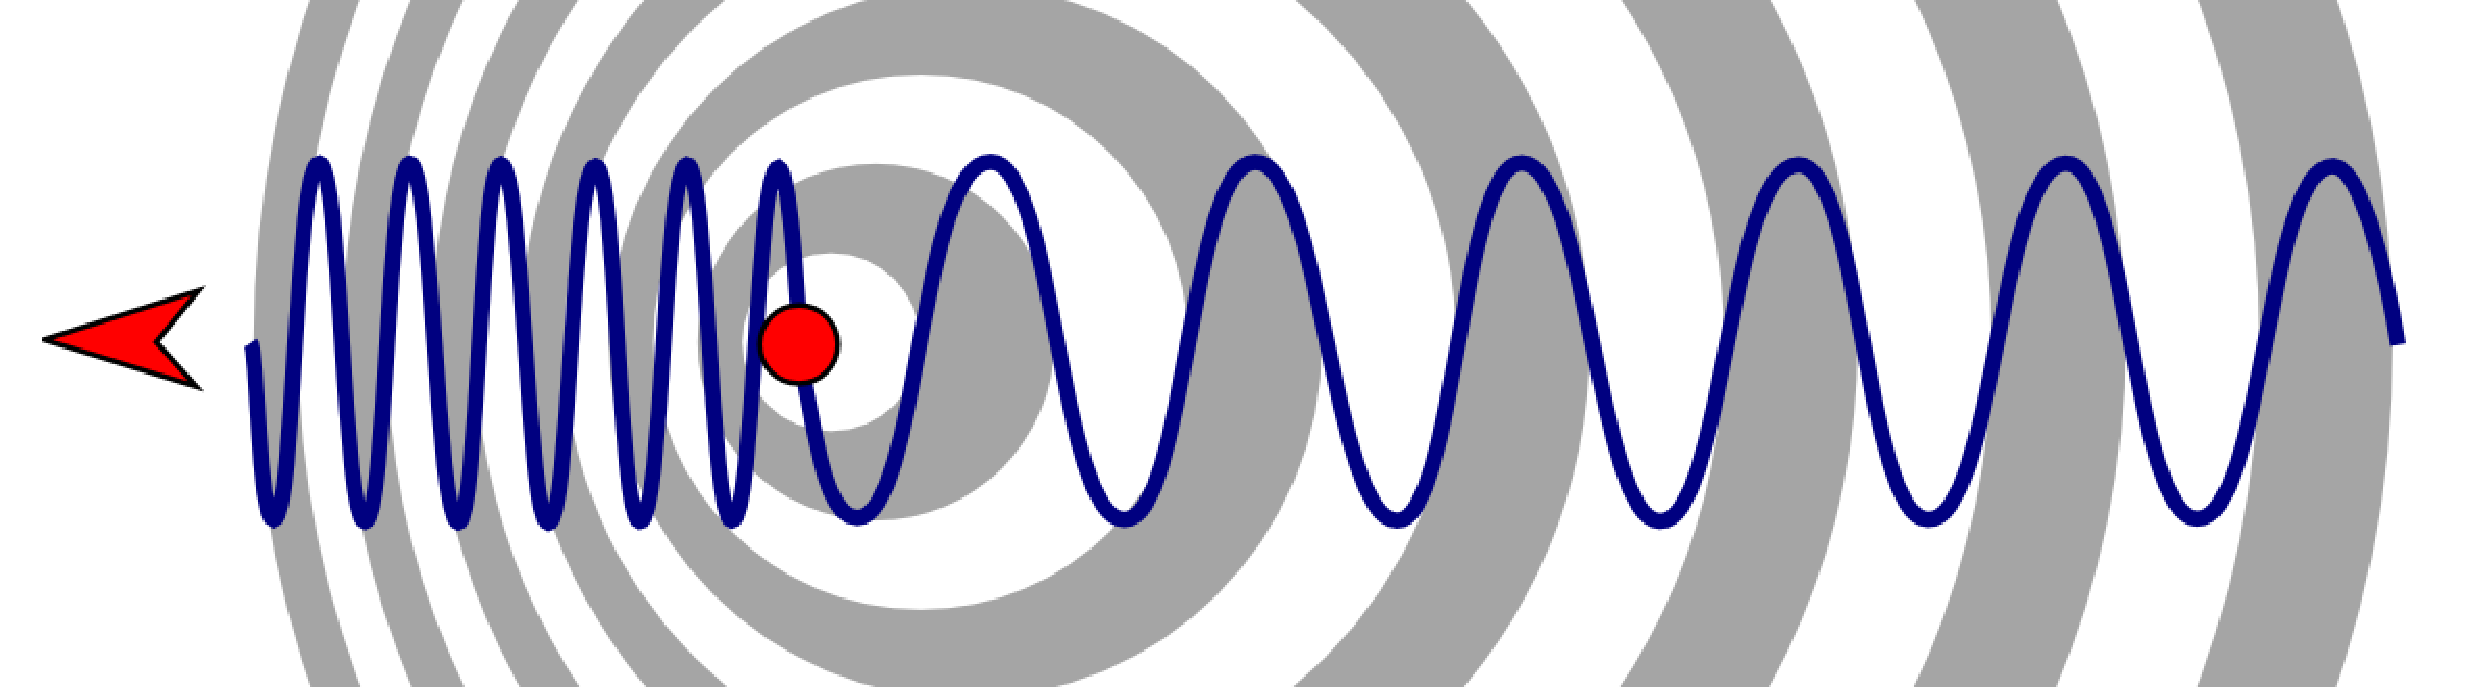
\includegraphics[width=.5\tw]{doppler-ef}
	\caption{Эффект Доплера}
	\label{doppler-ef}
\end{figure}

При $\Delta \lambda \ll \lambda_0$ с большой точностью выполняется следующее важное соотношение:\begin{equation}
	\beta \equiv \dfrac{v}{c} = \dfrac{\lambda - \lambda_0}{\lambda_0} \equiv \dfrac{\Delta \lambda}{\lambda_0},
	\label{eq:dopler-ef-simple}
\end{equation}
где $\lambda_0$~--- лабораторная длина волны излучения источника, а $\lambda$~--- наблюдаемая. 
В действительности же имеет место более общий случай: \imp{релятивистский эффект Доплера}, обусловленный проявлением СТО при $v \simeq c$, для которого формула~\eqref{eq:dopler-ef-simple} усложняется и принимает вид \begin{equation}
	\nu = \nu_0 \cdot \dfrac{\sqrt{1 - \beta^2}}{1 - \beta \cdot \cos\theta},
	\label{eq:dopler-ef-rel}
\end{equation}
где $\nu$~--- частота, с которой наблюдатель принимает волны, $\nu_0$~--- частота, с которой источник испускает волны, $v$~--- скорость источника, $\theta$~--- угол между направлением на источник и вектором скорости в системе отсчёта приёмника. Если источник радиально удаляется от наблюдателя, то $\theta = 0$, если приближается, то $\theta =\pi$. 

Стоит отметить, что~\eqref{eq:dopler-ef-simple} напрямую следует из \eqref{eq:dopler-ef-rel} при $\beta  \ll 1$.

\term{Красное смещение}~--- явление сдвига спектральных линий химических элементов в красную (длинноволновую) сторону обусловленное удалением галактик друг от друга. Параметр красного смещения определяется из наблюдаемой и лабораторной длин волн, как
\begin{equation}
	z = \dfrac{\lambda - \lambda_0}{\lambda_0}
\end{equation}

Доплеровское смещение длины волны в спектре источника, движущегося с лучевой скоростью $v_{r}$ и полной скоростью $v$,
\begin{equation}
z = \dfrac{1 + v_r / c}{\sqrt{1 - \beta^2}}.
\end{equation}

\term{Гравитационное красное смещение}~--- проявление эффекта изменения частоты излучения испущенного некоторым источником по мере удаления от массивных объектов, таких как звёзды и чёрные дыры. Наблюдается как сдвиг спектральных линий в излучении источников, близких к массивным телам, в красную область спектра. Гравитационное красное смещение определяется из формулы, выведенной Эйнштейном:
\begin{equation}
z_G=\dfrac{GM}{c^2 R}-\dfrac{GM}{c^2 r},
\label{eq:grav-red-shift}
\end{equation}
где $M$~--- масса гравитирующего тела, $R$~--- радиальное расстояние от центра масс тела до точки излучения (радиус источника), $r$~---  радиальное расстояние от центра масс тела до точки наблюдения. В случае, когда наблюдатель находится много дальше радиуса источника, т.\,е. выполняется соотношение $r \gg R$ формула~\eqref{eq:grav-red-shift} упрощается до \begin{equation}
	z_G \simeq \dfrac{GM}{c^2 R},
\end{equation}

\subsection{Световой поток. Альбедо}
Освещённость (плотность потока) --- мощность излучения, приходящаяся на единичную площадь. Освещённость обратно пропорционально квадрату расстояния до объекта:
\begin{equation}
E\sim \frac{1}{r^2},
\end{equation}
где $E$ --- освещённость (плотность потока) от объекта, $r$ --- расстояние до объекта.

Светимость --- мощность излучения, испускаемая с единичной площади поверхности объекта. Светимость вычисляется по следующей формуле:
\begin{equation}
E=\frac{L}{4\pi r^2},
\end{equation}
где $L$ --- полная светимость объекта.

Прежде всего световой поток является частным случаем \textit{теоремы Гаусса}. Общая формулировка:  поток излучения равен мощности, переносимой оптическим излучением через какую-либо поверхность. 
\begin{equation}
\Phi_e=\oint_SJ\cdot dS=\frac{dQ_e}{dt},
\end{equation}
где $J$ --- мощность светового потока, $dQ_e$~--- энергия излучения, переносимая через поверхность за время $dt$.


Альбедо($A$) --- характеристика отражательной способности поверхности какого-либо объекта. Альбедо является отношением отражённого светового потока к падающему на поверхность объекта. Тогда для нахождения поглощённой части излучения используется следующее соотношение:
\begin{equation}
E_{\text{п}}=E_0\cdot (1-A),
\end{equation}
где $E_{\text{п}}$ --- поглощённая часть излучения, $E_0$ --- приходящее излучение, $A$ --- альбедо.

А для отражённой части излучения можно использовать следующую формулу:
\begin{equation}
E_{\text{отр}}=A\cdot E_0,
\end{equation}
где $E_{\text{отр}}$ --- отражённая часть излучения.

Существует несколько видов альбедо --- \textit{геометрическое}, \textit{сферическое} и \textit{бондовское}. \textit{Геометрическое альбедо} равно отношению освещённости у Земли, создаваемой планетой в полной фазе, к освещённости, которую создал бы плоский абсолютно белый экран того же размера, что и планета, расположенный на её месте перпендикулярно лучу зрения и солнечным лучам. \textit{Сферическое альбедо} определяется как отношение светового потока, рассеянного телом во всех направлениях, к потоку, падающему на это тело. Может быть определено и для некоторого диапазона длин волн, и для всего спектра. Сферическое альбедо для всего спектра излучения называется \textit{альбедо Бонда}.
\subsection{Гравитационное линзирование}
\term{Гравитационное линзирование}~--- эффект, связанный с искривлением пути
\begin{wrapfigure}[9]{l}{0.35\tw}
	\centering
	\vspace{-.5pc}
	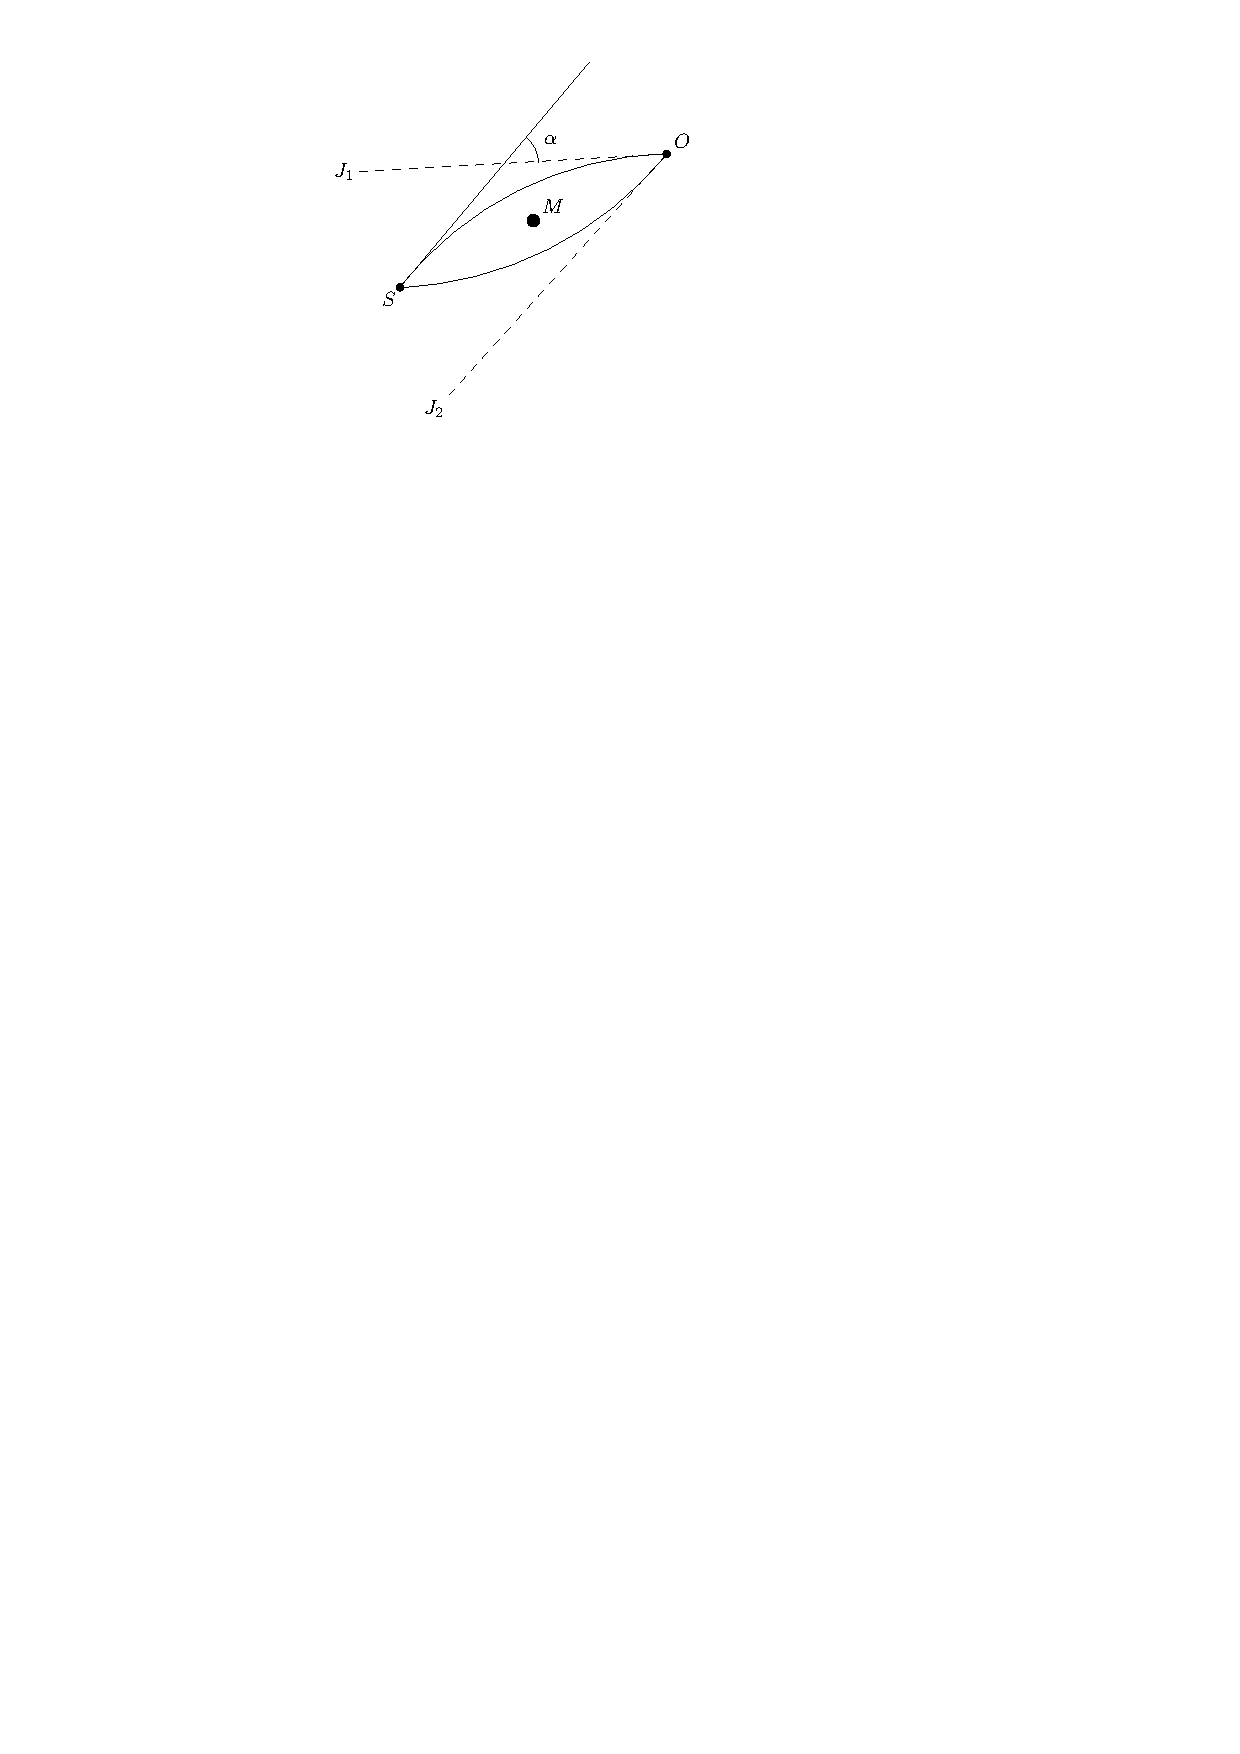
\includegraphics[width=0.35\tw]{grav-lens}
	\caption{Гравитационное линзирование}
	\label{grav-lens}
\end{wrapfigure}
распространения электромагнитного излучения гравитационным полем массивного тела или системы тел (галактик, скопления галактик, скопления тёмной материи).

На Рис.\,\ref{grav-lens} показано, как происходит гравитационное линзирование: $S$~--- источник электромагнитных волн, $O$~--- наблюдатель, $J_1$ и $J_2$~--- видимые положения источника, $M$~--- массивное тело массы $M$ и радиуса $R$.

Для угла преломления лучей $\alpha$ в ходе гравитационного линзирования справедлива формула
\begin{equation}
	\alpha = \frac{4 G M}{R c^2}.
\end{equation}
\subsection{Закон Хаббла}
\term{Закон Хаббла}~--- эмпирический закон, связывающий скорость удаления галактик и расстояние до них линейным образом. Описывается выражением \begin{equation}
V = H R,
\end{equation}
где $V$~--- скорость удаления галактики, $H=68$~км/$(\text{c} \cdot \text{Мпк})$~--- постоянная Хаббла, $R$~--- расстояние до галактики. 

При $v \ll c$ можно использовать приближение эффекта Доплера, тогда
\begin{equation}
V = c z,
\label{eq:hubble-speed}
\end{equation}
где $c$~--- скорость света, $z$~--- красное смещение.

Равенство \eqref{eq:hubble-speed} справедливо только при $z \ll 1$, а при б\'{o}льших значениях $z$ из-за эффектов СТО используется более сложная формула \begin{equation}
V = c \cdot \frac{(1 + z)^2 - 1}{(1 + z)^2 + 1}
\end{equation}
\subsection{Звёздные величины. Световой поток. Альбедо}

Звёздная величина --- безразмерная числовая характеристика яркости объекта, которая прежде всего является логарифмической шкалой. Известно, что увеличению светового потока в 100 раз соответствует уменьшение видимой звёздной величины ровно на 5 единиц. Тогда уменьшение звёздной величины на одну единицу означает увеличение светового потока в $\sqrt[5]{100}\approx 2.512$. Широко используется понятие \imp{абсолютной} звёздной величины. \term{Абсолютная звёздная величина} ($M$)~--- видимая звёздная величина($m$) с установленного расстояния от наблюдателя. Для звёзд~---~10~пк, для астероидов и комет~---~1~\au. Также звёздная величина может быть \textit{болометрической}~($m_{Bol}$). Это звёздная величина, при расчёте которой учитывается полное излучение во всех диапазонах электромагнитных волн. Найти болометрическую величину можно, зная болометрическую поправку:
\begin{equation}
	m + BC = m_{bol},
\end{equation}
где $BC$~--- болометрическая поправка.

Абсолютную звёздную величину звезды можно вычислить по следующей формуле:
\begin{equation}
	M = m + 5 - 5\lg r = m + 5 + 5 \lg \pi,
\end{equation}
где $M$~--- абсолютная звёздная величина, $m$~--- видимая звёздная величина, $r$~--- расстояние до звезды в парсеках, $\pi$~--- параллакс звезды.

Звёздную величину и освещённость объекта связывает \term{формула Погсона}:
\begin{equation}
	\frac{E_1}{E_2} = 10^{0.4(m_2 - m_1)}.
\end{equation}
Иначе,
\begin{equation}
m_1 - m_2 = 2.5 \lg \frac{E_2}{E_1},
\end{equation}
где $E_1$ и $E_2$~--- освещённость от объекта, $m_1$ и $m_2$~--- звёздная величина объекта.

\subsection{Энергия и импульс фотона}
\term{Фотон}~--- материальная, электрически нейтральная частица, квант электромагнитного поля (переносчик электромагнитного взаимодействия). В силу корпускулярно-волнового дуализма фотон можно рассматривать либо как частицу, либо как волну. Фотон не имеет массы, однако обладает энергией
\begin{equation}
	E = h \nu = \frac{h c}{\lambda}
\end{equation}
и импульсом, определяемом как
\begin{equation}
	p = \frac{E}{c} = \frac{h}{\lambda},
\end{equation}
где $h = 6.63 \cdot 10^{-34}~\text{Дж}\cdot\text{с}$~---  постоянная Планка.
\subsection{Формула Планка}

\term{Формула Планка} --- выражение для спектральной плотности мощности излучения абсолютно чёрного тела, применяемое  для интервала частот излучения  $[\nu, \nu + d \nu)$, которое было получено Максом Планком для равновесной плотности излучения $B(\nu,T)$. Полученное выражение записывается следующим образом, где $\nu$ --- частота излучения, $T$ --- температура, $h$ --- постоянная Планка, $k$ --- постоянная Больцмана, $c$ --- скорость света:
\begin{equation}\label{Planck's formula}
B(\nu,T)=\frac{2h\nu^3}{c^2}\cdot \frac{h\nu}{\exp\left(\frac{h\nu}{kT}\right)-1}.
\end{equation}

Если записать закон излучения Планка (\ref{Planck's formula}) для длин волн, то функция примет следующий вид:
\begin{equation}\label{Planck's formula2}
B(\lambda,T)=\frac{2hc^2}{\lambda^5} \cdot \frac{1}{\exp\left(\frac{hc}{\lambda kT}\right)-1}
\end{equation}

Стоит заметить, что при переходе функции к длинам волн меняется не только частота на длину волны, но и интервал. 

\begin{figure}[h!]
\begin{center}
 \begin{tikzpicture}
  \begin{axis}[
  		ymax=4.35e+14,
  		xmax=1.5,
  		axis x line=bottom,
		axis y line=left, 
		xlabel={Длина волны $\lambda$,~мкм}, 
		ylabel={Мощность излучения $B(\lambda)$,~Вт/$\text{м}^2\cdot$~нм},
		width=7.5cm, 
		height=7.5cm, 
		no markers, 
		minor x tick num = 1,
		minor y tick num = 1,
		grid = both,
		line width=.7pt,
		cycle list = {
			{smooth,green!50!black,solid},
			{smooth,red,solid},
			{smooth,blue,solid},
			{smooth,brown,solid},
			{smooth,black,solid},
			{smooth,red,solid},
			{smooth,brown,solid}
		}
]
   \addplot table[x=l, y=t10] {data/data2.txt}
   node at (axis cs:0.29, 4.2e+14)
{$5500$K};
   \addplot table[x=l, y=t9] {data/data2.txt}node at (axis cs:0.33, 2.55e+14)
{$5000$K};
   \addplot table[x=l, y=t8] {data/data2.txt}node at (axis cs:0.364, 1.475e+14)
{$4500$K};
   \addplot table[x=l, y=t7] {data/data2.txt}node at (axis cs:0.415, 8.3e+13)
{$4000$K};
   \addplot table[x=l, y=t6] {data/data2.txt}node at (axis cs:0.44, 4.5e+13)
{$3500$K};
  \end{axis}
 \end{tikzpicture}
\end{center}
\caption{Кривые спектральной плотности потока излучения абсолютно чёрных тел с разной температурой}\label{pic:wien-law}
\end{figure}

Формула Планка появилась тогда, как стало ясно, что формула Рэлея — Джинса удоволетворительно описывает излучение только в области длинных волн, а с убыванием длин волн даёт сильные расхождения с эмпирическими данными. Формула Рэлея-Джинса для длин волн записывается таким образом:
\begin{equation}\label{Ray-Jean}
B(\lambda,T)=\frac{2ckT}{\lambda^4}
\end{equation}

Если формулу Рэлея — Джинса записать для частоты излучения, то формула примет данный вид:
\begin{equation}\label{Ray-Jean2}
B(\nu,T)=\frac{2\nu^2 kT}{c^2}
\end{equation}

Также формулы (\ref{Ray-Jean}) и (\ref{Ray-Jean2}) можно записать для коротковолновой и высокочастотной области:
\begin{equation}
U(\lambda,T)\approx\frac{2hc^2}{\lambda^5}\exp\left(-\frac{hc}{\lambda kT}\right)
\end{equation}
\begin{equation}
U(\nu,T)\approx\frac{2h\nu^3}{c^2}\exp\left(-\frac{h\nu}{kT}\right)
\end{equation}
\subsection{Шкала электромагнитных волн}


\term{Гамма излучение} возникают при радиоактивных распадах ядер, при торможении электронов энергией более $10^5$~эВ и при других взаимодействиях элементарных частиц. Используются в гамма-дефектоскопии, при изучении свойств вещества.

\term{Рентгеновские лучи} излучаются при большом ускорении электронов, например их торможение в металлах. Получают при помощи рентгеновской трубки: электроны в вакуумной трубке ускоряются электрическим полем при высоком напряжении, достигая анода, при со­ударении резко тормозятся. При торможении электроны движут­ся с ускорением и излучают электромагнитные волны с малой длиной. 

\begin{figure}[!h]
\centering
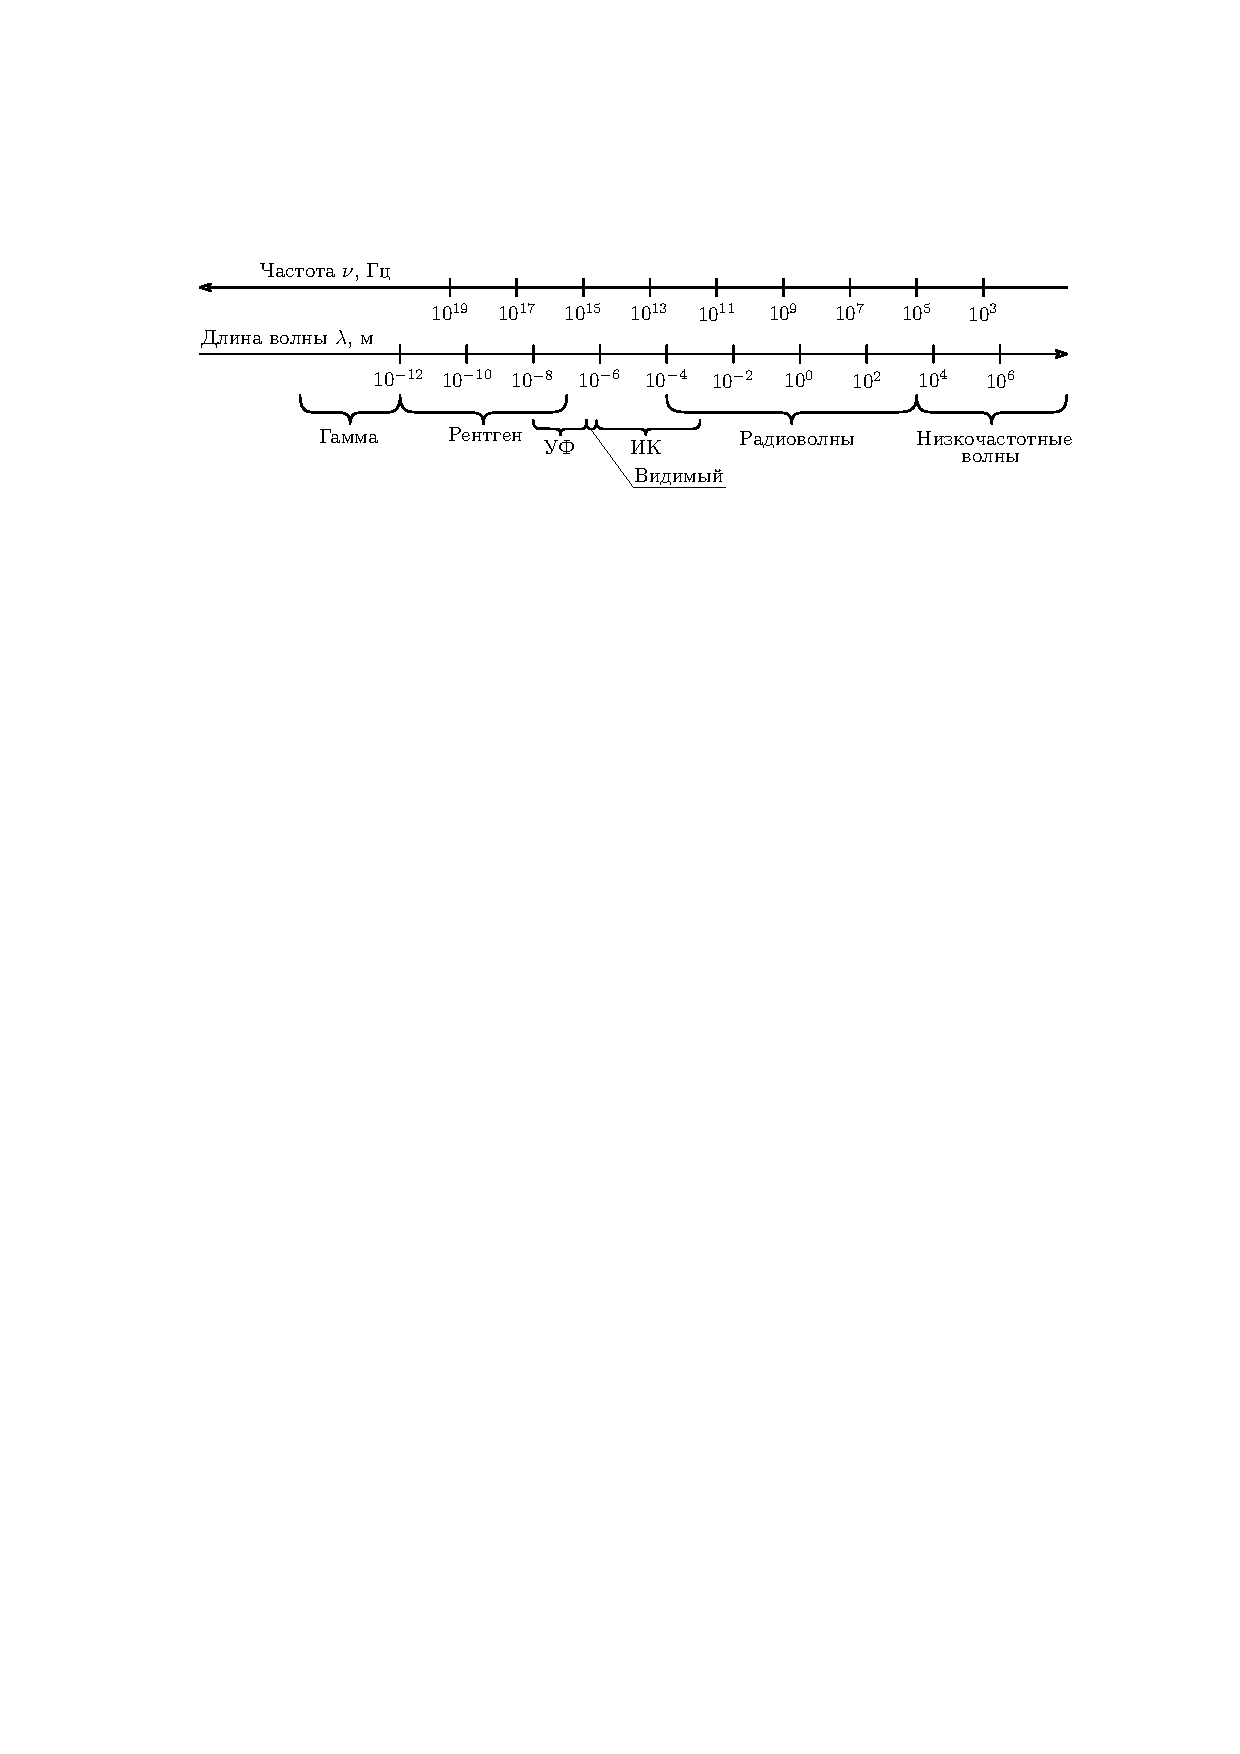
\includegraphics[width = 1\textwidth]{scale-wave.pdf}
\caption{Шкала электромагнитных волн}
\end{figure}
\term{Ультрафиолетовые лучи}~--- излучение Солнца, ртутных ламп и т.\,п. Используются в ультрафиолетовой микроскопии, в медицине.

\term{Видимое излучение}~--- часть электромагнитного излучения, воспринимаемая глазом (от фиолетового до от красного).

\term{Инфракрасное излучение}~--- тепловое, излучается любым нагретым телом.

\term{Радиоволны} используются повсеместно в обычной жизни, это и сотовая связь, и радиолокация, и спутниковая связь, и многое другое.

\term{Низкочастотные волны}~--- диапазон, традиционно используемый в электротехнике. В промышленной электроэнергетике используется частота 50~Гц, на~которой осуществляется передача электрической энергии по линиям и преобразование напряжений трансформаторными устройствами.
\subsection{Специальная теория относительности. Аберрация}

Обычно в СТО рассматриваются две инерциальные системы $S$ и $S'$. Время и координаты некоторого события, измеренные относительно системы $S$, обозначаются как $(t, x, y, z)$, а координаты и время этого же события, измеренные относительно системы $S'$, как $(t', x', y', z')$. Удобно считать, что координатные оси систем параллельны друг другу, и система $S'$ движется вдоль оси $x$ системы $S$ со скоростью $v$. Одной из задач СТО является поиск соотношений, связывающих $(t', x', y', z')$ и $(t, x, y, z)$, которые называются \textit{преобразованиями Лоренца}. Общий вид преобразований Лоренца в векторном виде, когда скорость систем отсчёта имеет произвольное направление:

\begin{equation}
t'=\gamma\cdot \left(t-\frac{\vec{rv}}{c^2}\right),
\end{equation}
\begin{equation}
\vec{r}\,'=r-\gamma \vec{v}t+(\gamma-1)\cdot\frac{(\vec{rv})\vec{\mathbf v}}{v^2},
\end{equation}
где  $\gamma=1/{\sqrt {1-\vec{v}^{\,2}/c^{2}}}$, $\vec{r}$ и $\vec{r}\,'$ --- радиус-векторы события относительно систем $S$ и $S'$.

Если сориентировать координатные оси по направлению относительного движения инерциальных систем и выбрать это направление в качестве оси $x$, то преобразования Лоренца примут следующий вид: 
\begin{equation}
t'=\frac{t-\frac{v}{c^2}x}{\sqrt{1-\frac{v^2}{c^2}}},\quad\text{  } x'=\frac{x-vt}{\sqrt{1-\frac{v^2}{c^2}}},\quad\text{  } y'=y,\quad\text{  } z'=z,
\end{equation}
где $c$ --- скорость света.

 При скоростях много меньше скорости света $(v\ll c)$ преобразования Лоренца переходят в \textit{преобразования Галилея}:
\begin{equation}
 t'=t,\quad\text{  } x'=x-vt,\quad\text{  }  y'=y,\quad\text{  }  z'=z
\end{equation}
 
\term{Аберрация} --- явление, состоящее в том, что движущийся наблюдатель видит светило не в том направлении, в котором он видел бы его в тот же момент, если бы находился в покое, причём смещается светило в сторону движения наблюдателя. Происходит это из-за конечности скорости света и из-за изменения системы отсчёта для наблюдателя.  
Угол аберрационного смещения можно найти по следующей формуле:
\begin{equation}\sigma=\frac{v}{c}\sin\theta,
\end{equation}
где $v$ --- скорость наблюдателя, $\theta$ --- угол между направлением вектора скорости наблюдателя и направлением на объект. 
\subsection{Спектральные классы звёзд}
\begin{table}[h!]
\centering
\footnotesize
\renewcommand{\arraystretch}{1.4}
\renewcommand{\tabcolsep}{0pt}
\begin{tabularx}{\tw}{|C{0.1}|C{0.3}|C{0.23}|C{0.13}|C{0.13}|C{0.13}|}
\hline
{\bfseries Класс} & {$\mathbf{T}$, К} & {\bfseries Цвет} & {$\mathbf{M}$, $M_{\odot}$} & {$\mathbf{R}$, $R_{\odot}$} & {$\mathbf{L}$, $L_{\odot}$}\\
\hline
O & $3 \times 10^4$ --- $6 \times 10^4$ & Голубой & 60 & 15 & $1.4 \times 10^6$\\

B & $1 \times 10^4$ --- $3 \times 10^4$ & Бело-голубой & 18 & 7 & $2 \times 10^4$\\

A & $7.5 \times 10^3$ --- $1 \times 10^4$ & Белый & 3.1 & 2.1 & 80\\

F & $6 \times 10^3$ --- $7.5 \times 10^3$ & Жёлто-белый & 1.7 & 1.3 & 6\\

G & $5 \times 10^3$ --- $6 \times 10^3$ & Жёлтый & 1.1 & 1.1 & 1.2\\

K & $3.5 \times 10^3$ --- $5 \times 10^3$ & Оранжевый & 0.8 & 0.9 & 0.4\\

M & $2 \times 10^3$ --- $3.5 \times 10^3$ & Красный & 0.3 & 0.4 & 0.04\\
\hline
\end{tabularx}
\caption{Современная спектральная классификация звёзд}
\end{table}

Помимо основных спектральных классов звёзд существуют и дополнительные:
\begin{enumerate}[1)]
\item Класс W --- звёзды Вольфа-Райе, очень тяжёлые яркие звёзды с температурой порядка $70000$~К и интенсивными эмиссиоными линиями спектра.
\item Класс L --- звёзды или коричневые карлики с температурой $1500 - 2000$~К и соединениями металлов в атмосфере.
\item Класс T --- метановые коричневые карлики с температурой $700 - 1500$~К.
\item Класс Y ---  очень холодные (метано-аммиачные) коричневые карлики с температурой ниже $700$~К.
\item Класс C --- углеродные звёзды, гиганты с повышенным содержанием углерода. Ранее относились к классам R и N.
\end{enumerate}

Мнемонические правила для запоминания спектральных классов:
\begin{enumerate}[1)]
\item\textbf{O}h \textbf{B}e \textbf{A} \textbf{F}ine \textbf{G}irl, \textbf{K}iss \textbf{M}e \textbf{R}ight \textbf{N}ow \textbf{S}weetheart.
\item\textbf{W}ell, \textbf{O}nce \textbf{B}ritish \textbf{A}stronomer has \textbf{F}ound \textbf{G}alaxy, \textbf{K}new \textbf{M}ass, \textbf{L}ength, \textbf{T}erm.
\item Вообразите: \textbf{О}дин \textbf{Б}ритый \textbf{А}нгличанин \textbf{Ф}иники \textbf{Ж}евал \textbf{К}ак \textbf{М}орковь --- \textbf{Р}азве \textbf{Н}е \textbf{С}мешно?
\end{enumerate}

\term{Диаграмма Герцшпрунга-Рассела} показывает зависимость между светимостью, спектральным классом и температурой поверхности звезды. 

\begin{figure}
	\centering
%	\begin{tikzpicture}
% 		\begin{axis}[
% 						height	=	12cm,
% 						width	=	10cm,
% 						ymax	=	15.,
% 						ymin	=	-10.,
% 						y dir	=	reverse,
% 						xmax	=	2.,
% 						xmin	=	-.5,
% 						axis x line* = bottom,
% 						axis y line* = right,
% 						xlabel=$B-V$,
% 						y label style = {at={(axis description cs: 1.2, 0.5)}, rotate=180}, 
% 						ylabel	=	{Абсолютная звёздная величина $M$, $~^m$}
% 					]
%%			\addplot+[only marks, mark = o, mark options={scale=0.2, black}] table[x=f, y=m]{data/light-curve-D-Cep.txt};
% 		\end{axis}
% 		\begin{semilogyaxis}[	
% 						height	=	12cm,
% 						width	=	10cm,
% 						ymax	=	8.312e5,
% 						ymin	=	8.312e-5,
% 						xmax	=	2.,
% 						xmin	=	-.5,
% 						minor x tick num = 0,
% 						minor y tick num = 01,
% 						xtick = {-0.264, 0, 0.3, 0.58, 0.791, 1.57},
% 						xticklabels = {B0, A0, F0, G0, K0, M0},
% 						axis x line* = top,
% 						axis y line* = left,
% 						xlabel	=	{Спектральный класс}, 
% 						x label style = {at={(axis description cs: 0.5, 1.11)}, rotate=0},
% 						ylabel	=	{Светимость $L$, $L_\odot$},
% 						ymajorgrids	 =	false,
% 						xmajorgrids	 =	false	
%    				]
%		\end{semilogyaxis}
% 	\end{tikzpicture}
	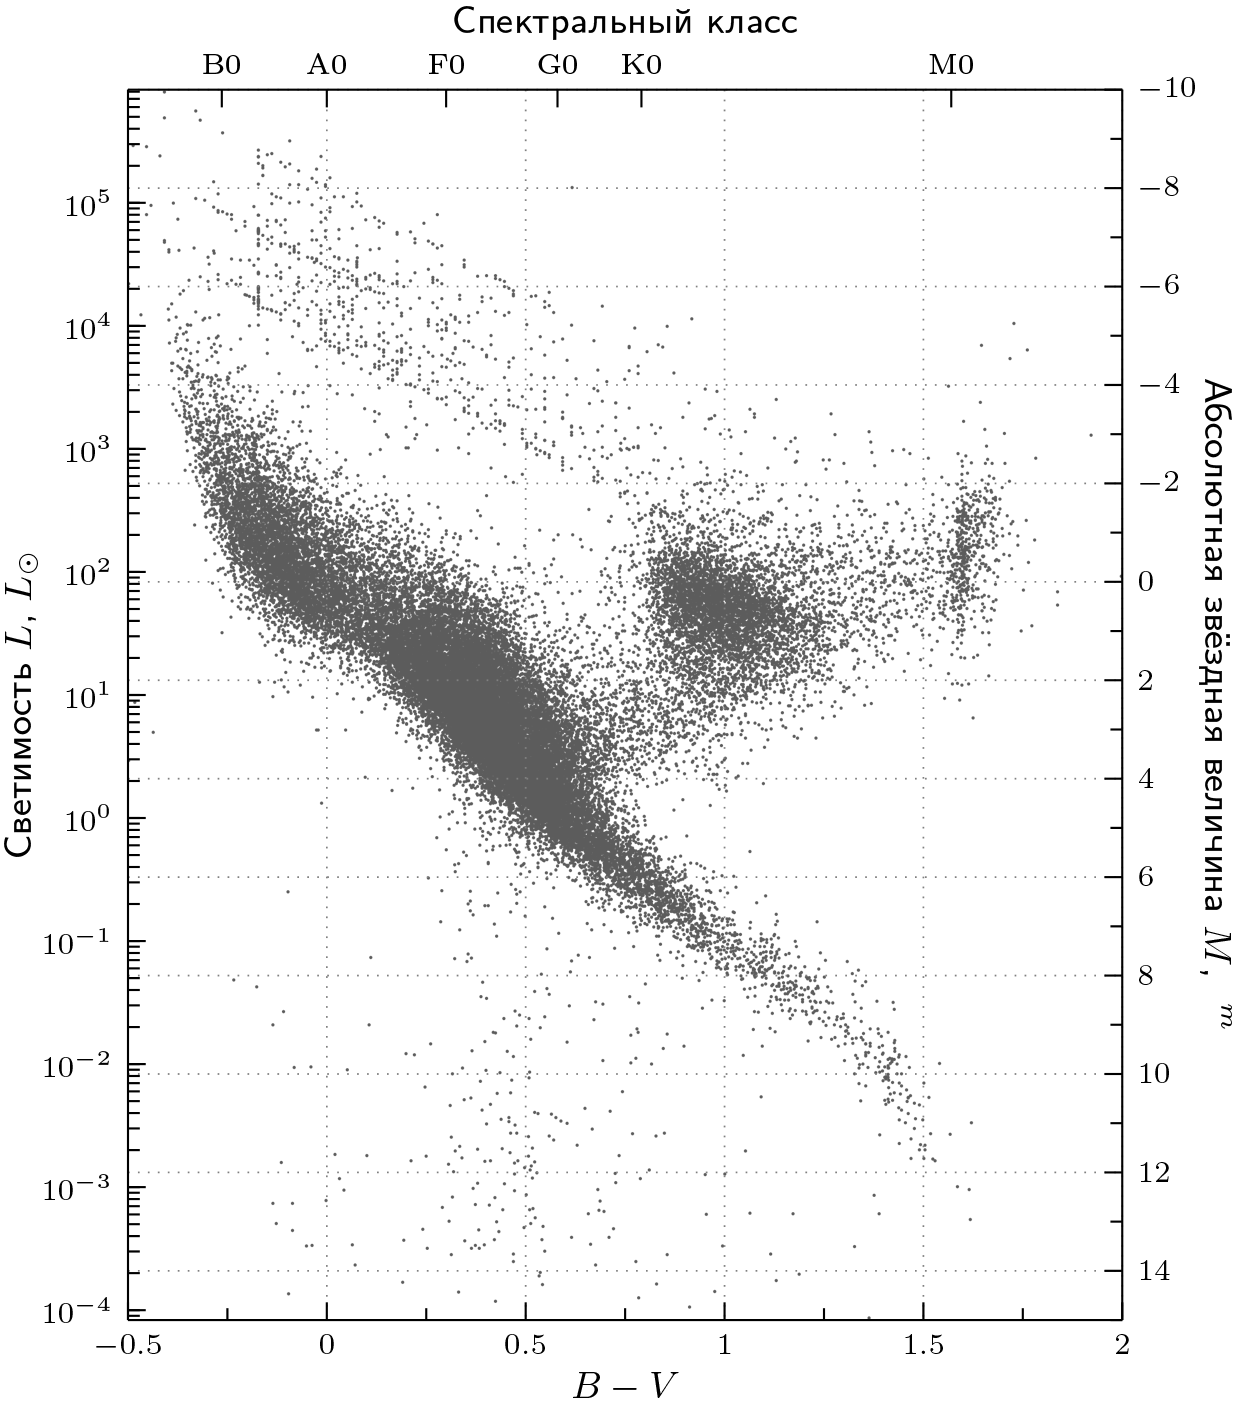
\includegraphics[width=10cm]{gr}
 	\caption{Диаграмма Герцшпрунга--Рассела}
 	\label{pic:d-cep}
\end{figure}


Была предложена примерно в 1910 году независимо Эйнаром Герцшпрунгом и Генри Расселом. Диаграмма используется для классификации звёзд и соответствует современным представлениям о звёздной эволюции.

Около $90 \%$ звёзд находятся на главной последовательности. Их светимость обусловлена термоядерными реакциями превращения водорода в гелий. Выделяется также несколько ветвей проэволюционировавших звёзд --- гигантов, в которых происходит горение гелия и более тяжёлых элементов. В левой нижней части диаграммы находятся полностью проэволюционировавшие белые карлики.


\subsection{Закон Стефана-Больцмана}
\term{Закон Стефана~--- Больцмана} определяет зависимость плотности мощности излучения абсолютно чёрного тела (АЧТ) $u$ от его температуры $T$:
\begin{equation}
u = a T^4,
\end{equation} 
где $a$~--- некая универсальная константа.
Отсюда полная светимость АЧТ с площадью поверхности $S$
	\begin{equation}
	L = S \sigma T^4,
	\label{eq:steff-bol-law}
\end{equation}
константа $\sigma$ называется \term{постоянной Стефана-Больцмана}.
  
Важно отметить, что \imp{закон Стефана-Больцмана}~--- прямое следствие формулы Планка \eqref{Planck's formula}, так как
\begin{equation}
	\sigma T^4 = \int\limits^\infty_0 B(\lambda, T)\,d\lambda \int\limits_0^{\pi/2} \sin \varphi\, d\varphi \int\limits_0^{2\pi} \cos \varphi\, d\theta = \pi \int\limits^\infty_0 B(\lambda, T)\,d\lambda,
\end{equation}
откуда $\sigma = (2\pi^5k^4)/(15c^2h^3) = 5.67 \cdot 10^{-8}~\text{Вт}/(\text{м}^2\cdot \text{К}^4)$.

%Для АЧТ сферической формы с радиусом $R$ формула~\eqref{eq:steff-bol-law} принимает вид
%\begin{equation}
%L=4\pi R^2\sigma T^4.
%\end{equation}
Для звёзд главной последовательности выполняется соотношение $L \sim M^{\alpha}$, где~$\alpha$~--- коэффициент пропорциональности, который зависит от массы звезды следующим образом:
\begin{align*}
\alpha &= 2.5, \quad M < 0.43 M_\odot; & 
\alpha &= 4, \quad 0.43 M_\odot < M < 2 M_\odot;\\ 
\alpha &= 3.2, \quad 2 M_\odot < M < 20 M_\odot; & 
\alpha &= 1, \quad M > 20 M_\odot.
\end{align*}
Также существует примерная зависимость светимости звёзды от её радиуса, имеющая вид  $L\sim R^{5.2}$.
\subsection{Солнце}
\subsubsection*{Общая информация}

\textit{Солнце} --- центральное тело Солнечной системы. В нём сосредоточено 99,866\%  массы Солнечной системы. Солнце состоит из водорода (73\% от массы), гелия (25\%) и других элементов с меньшим содержанием: железа, никеля, азота, кислорода, кремния, серы, магния, углерода, неона, кальция, хрома и др.

По спектральной классификации Солнце --- звезда типа G2V (жёлтая звезда главной последовательности). Температура поверхности Солнца  примерно $5 800$~К, поэтому Солнце светит почти в белом свете, но прямой свет Солнца у поверхности Земли приобретает жёлтый оттенок из-за рассеяния и поглощения коротковолновой части спектра в атмосфере.

Солнце вырабатывает энергию путём термоядерного синтеза. Каждую секунду в ядре около 4 млн тонн веществе превращается в лучистую энергию.

\subsubsection*{Строение Солнца}

В центре Солнца находится ядро радиусом $150 $ --- $ 180$ тыс. км, в котором идут термоядерные реакции. Плотность  вещества в ядре $1.5\times 10^5~\text{кг}/\text{м}^3$, температура в центре ядра около $1.5\times 10^7$~К.

Над ядром, на расстояниях примерно от 0.2 --- 0.25 до 0.7 радиусов Солнца от его центра, находится зона лучистого переноса. В этой зоне перенос энергии происходит главным образом с помощью  излучения поглощения фотонов. Перепад температур в этой зоне от $2\times10^6$~К сверху до $7\times10^6$~К снизу.

Над зоной \textit{лучистого  переноса} (радиоактивная зона) находится конвективная зона. Этой слой толщиной примерно $2\times10^5$~км, в котором перенос энергии к поверхности совершается движением самого вещества. При приближении к поверхности конвективной зоны температура падает до 5800 К.

\textit{Фотосфера} --- видимая поверхность Солнца, по которой определяется размер Солнца. Эффективная температура фотосферы примерно 5780 К.

\textit{Хромосфера} --- внешняя оболочка Солнца толщиной около 2000 км, окружающая фотосферу. Из хромосферы происходят горячие  выбросы вещества --- \textit{спикулы}. Температура хромосферы увеличивается с высотой до $2\times10^4$~К.

\textit{Солнечная корона} --- последний внешний слой Солнца, который состоит из протуберанцев и энергетических  извержений, образующих солнечный ветер. Средняя температура короны $1-2\times10^6$~К, а в некоторых частях достигает  и $20\times10^6$~К. Столь высокая температура обусловлена процессами, происходящими в магнитном поле звезды. Однако, несмотря на столь высокую температуру, корона видна лишь во время солнечных затмений, так как плотность её очень мала.
  
  
  
\begin{figure}[h!]
\begin{center}
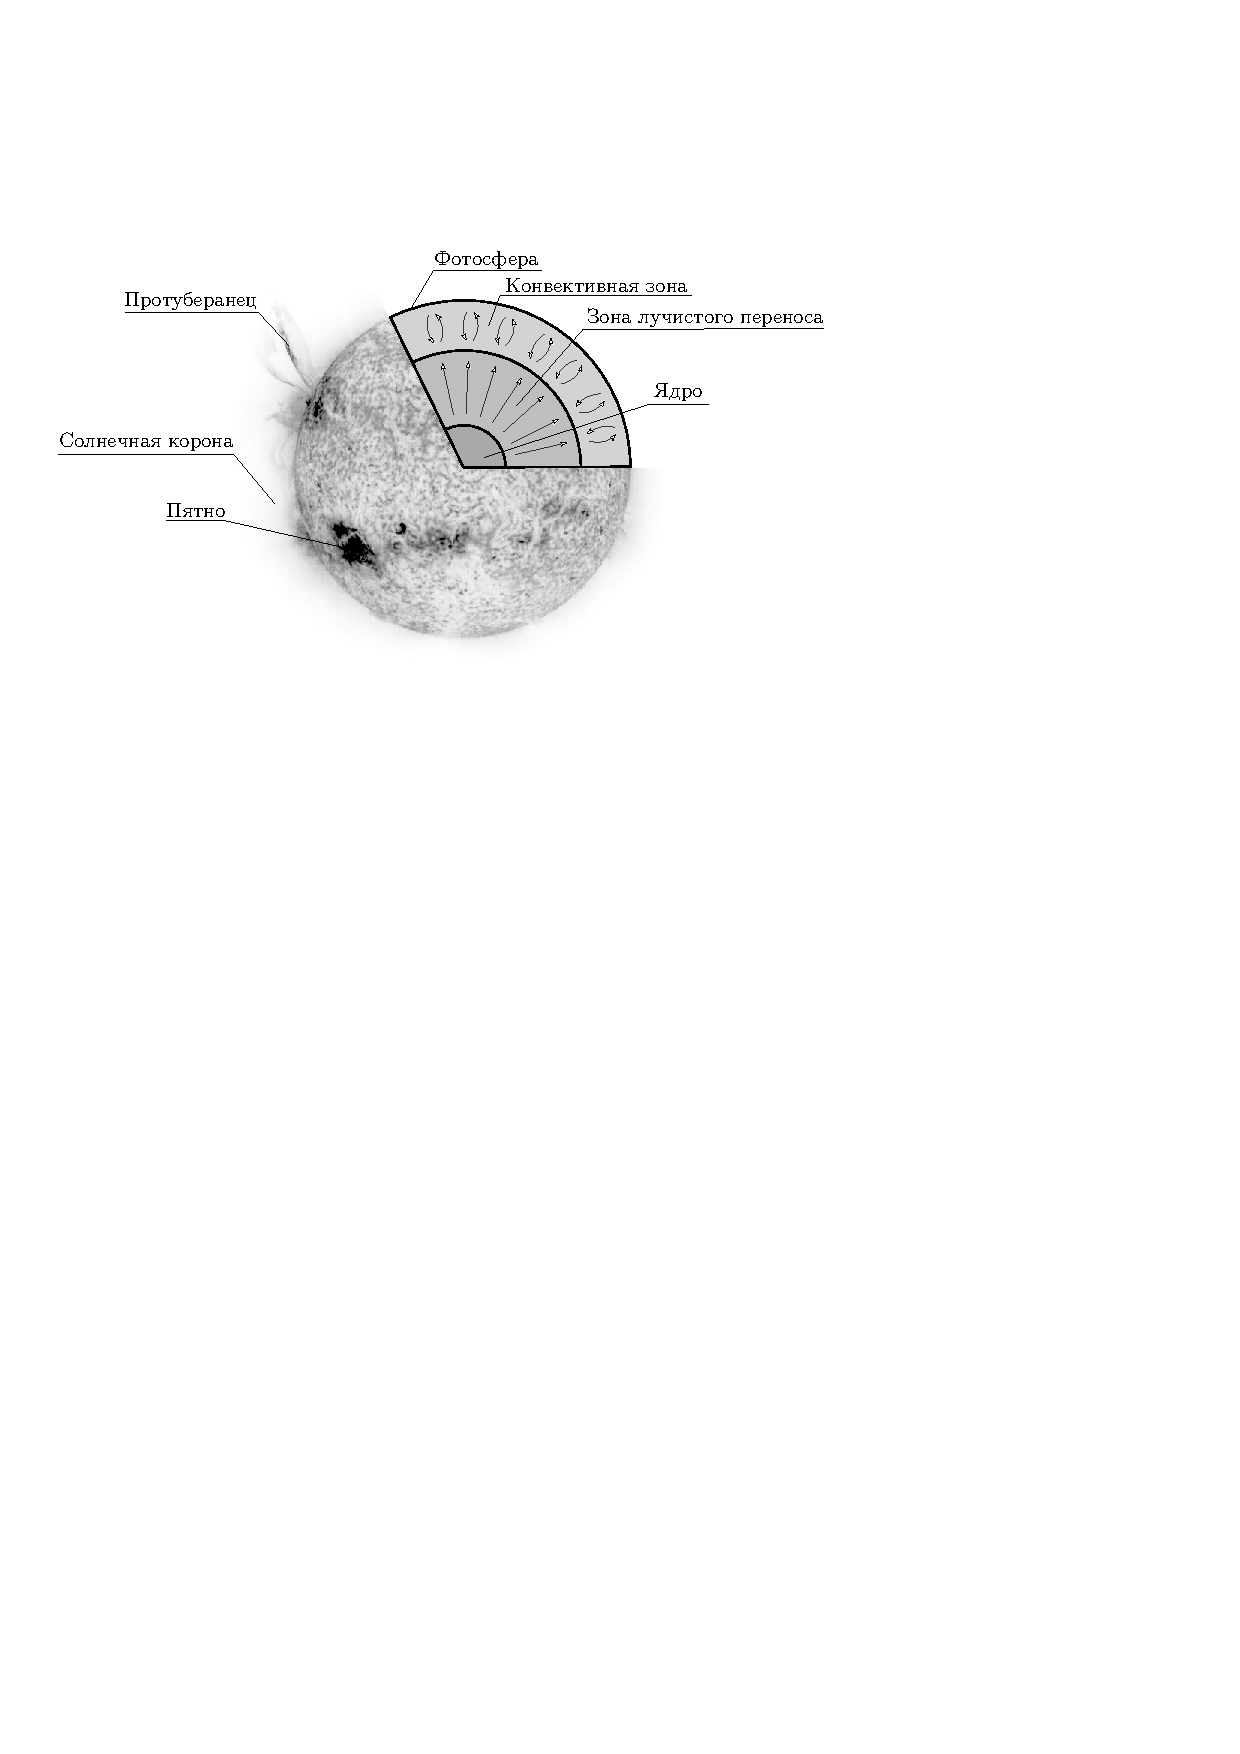
\includegraphics[width=0.65\textwidth]{sun}
\caption{Строение Солнца}
\end{center}
\end{figure}

Солнце вращается не твёрдотельно --- угловая скорость на разных широтах разная, при удалении от экватора она уменьшается. Период обращения Солнца на разных широтах можно найти, наблюдая за солнечными пятнами и другими образованиями. На экваторе период вращения состовляет 25.05 суток, к полюсу он увеличивается до 34 суток. По наблюдениям за пятнами в течение длительного периода при помощи метода наименьших квадратов можно найти зависимость углового перемещения пятна за сутки от гелиографической широты:
\begin{equation}
\Delta\lambda=14.37^{\circ}-2.7^{\circ}\sin^2\varphi,
\end{equation}
где $\Delta\lambda$ --- угловое перемещение пятна, $\varphi$ --- гелиографическая широта.

Вышеприведённая формула верна только для не очень больших значений широт ($\varphi<40^{\circ}$).
\subsection{Переменные звёзды}
\term{Переменные звёзды}~--- звёзды, у которых наблюдаются колебания блеска.   Для отнесения звезды к разряду переменных достаточно, чтобы блеск звезды хотя бы однажды претерпел изменение.

Переменные звёзды делятся на две большие группы: \imp{затменные} и \imp{физические}, причём физические подразделяются на \imp{пульсирующие} и \imp{эруптивные}.

К \term{пульсирующим} переменным  относят те звёзды, переменность которых вызвана процессами, происходящими в их недрах. Эти процессы приводят к периодическому изменению блеска звезды, а вместе с ним и других характеристик звезды~--- температуры поверхности, радиуса фотосферы и пр. Период переменности заключён в пределе от нескольких долей суток до нескольких лет. Абсолютную звёздную величину  и период связывает следующая формула:
\begin{equation}
	M = -1.01^m - 2.97\lg T,
\end{equation}
где $T$~--- период, выраженный в сутках, а $M$~--- абсолютная звёздная величина.

Классический пример пульсирующих переменных звёзд --- цефеиды.

\begin{figure}[h!]
\begin{center}
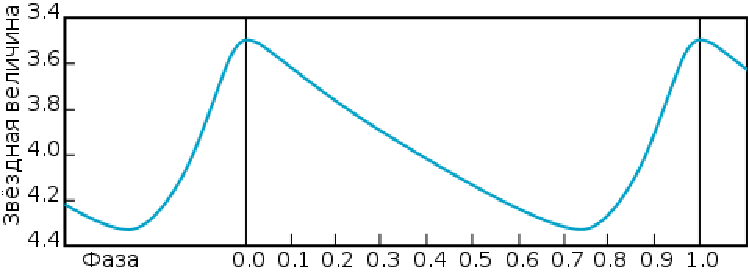
\includegraphics[width=0.7\tw]{var-stars}
\caption{Кривая блеска $\delta$ Цефея}
\end{center}
\end{figure}

К \term{эруптивным} переменным звёздам относятся звёзды, меняющие свой блеск нерегулярно или единожды за время наблюдений. Все изменения блеска эруптивных звёзд связывают с бурными процессами и вспышками в их хромосферах и коронах.

\term{Затменно-переменные} звёзды --- системы из двух звёзд, суммарный блеск которых периодически изменяется с течением времени. Причиной изменения блеска могут быть затмения звёзд друг другом, или изменение их формы взаимной гравитацией в тесных системах.

На всех кривых блеска (Рис.~\ref{var-stars}) заметны два минимума: глубокий (главный), соответствующий затмению главной звезды спутником, и слабый (вторичный), возникающий, когда главная звезда затмевает спутник.

%\begin{figure}[h!]
%	\centering
%	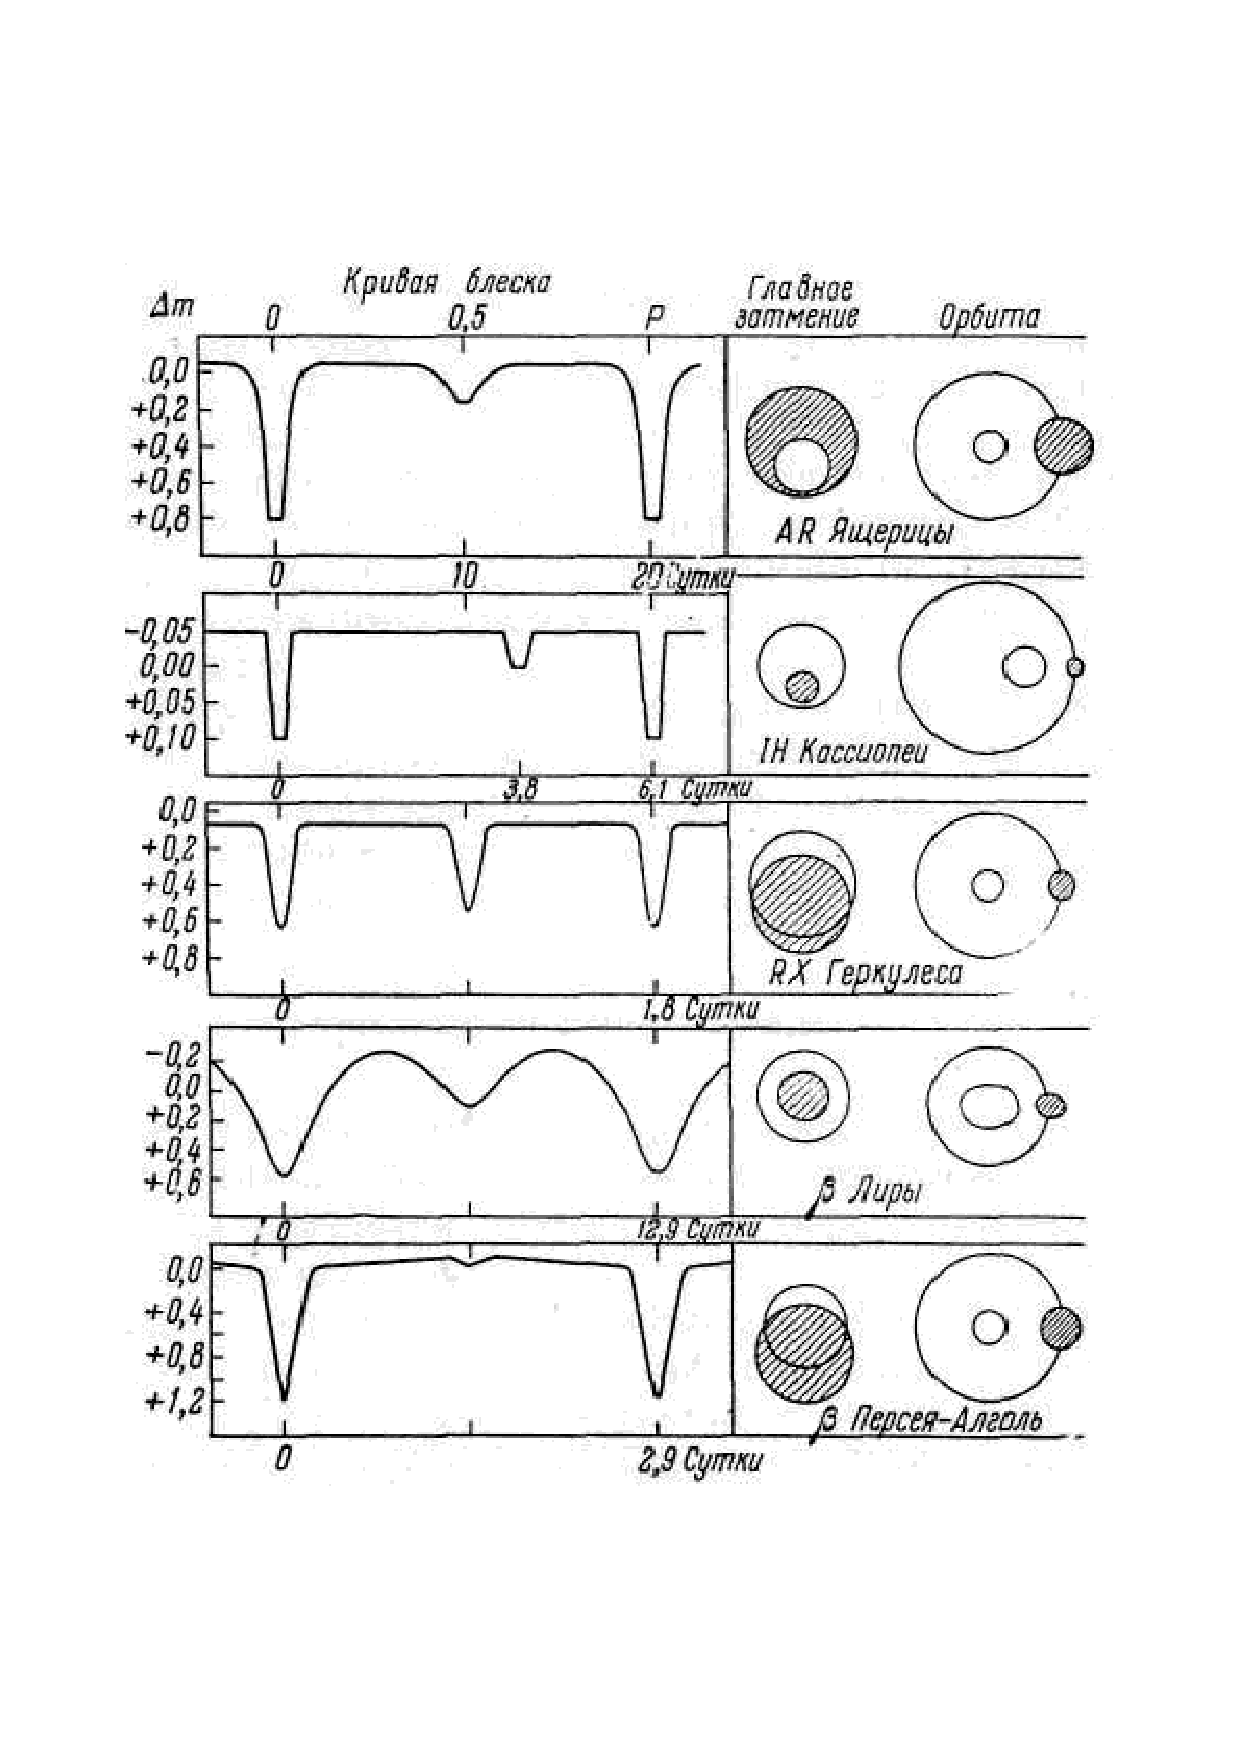
\includegraphics[width=0.8\tw]{var-stars2}
%	\caption{Кривые блеска некоторых затменно-переменных звёзд}
%	\label{var-stars}
%\end{figure}

\begin{figure}[!h]
\centering
 \begin{tikzpicture}
 \begin{axis}[
 no markers,
% xlabel={Прямое восхождение $\alpha^h$}, 
% ylabel={Склонение $\delta^{\circ}$},
 minor x tick num = 1,
 minor y tick num = 1,
 grid = both,
 line width=.7pt, 
% extra y ticks={23.44, -23.44},
 ymax=1.02,
 ymin=0.65,
 xmax=1,
 xmin=0,
% xtick={0,4,8,12,16,20,24}
 ]
% \addplot [domain=0:24, samples=100]{atan(sin(x*15)*tan(23.44))}; 
	\addplot table{data/light-curve-W-UMa.txt};
 \end{axis}
 \end{tikzpicture}
 \caption{График зависимости склонения от прямого восхождения Солнца}
\end{figure}




\subsection{Закон смещения Вина}
\term{Закон смещения Вина} --- закон, устанавливающий зависимость длины волны от температуры чёрного тела, на которой поток излучения энергии чёрного тела достигает своего максимума.

Длину волны, на которой интенсивность излучения абсолютно чёрного тела достигает своего максимума, можно определить по следующей формуле:
\begin{equation}
\lambda_{max} \approx \frac{b}{T},
\end{equation}
где $b \simeq 0.0029~\text{м} \cdot \text{К}$~--- \imp{постоянная Вина} равная

Данная формула получается путём нахождения экстремума \imp{функции Планка} для абсолютно чёрного тела, записанного для длин волн (\ref{Planck's formula2}).


\newpage
\section{Оптика}
\subsection{Схемы телескопов}
Телескопв по своей оптической схеме делятся на 3 типа:
\begin{enumerate}
\item Рефлекторы или диоптрические
\item Рефракторы или катаптрические
\item Катадиоптрические
\end{enumerate}

\term{Рефлектор} (зеркальный телескоп)~---  оптический телескоп, использующий в качестве светособирающего элемента зеркало.

\term{Рефрактор} (линзовый телескоп)~---  оптический телескоп, в котором для собирания света используется система линз.

\term{Катадиоптрический} (зеркально-линзовый) \textit{телескоп}~--- оптический телескоп, в котором используется как система линз, так и зеркал.

Ниже представлены схемы оптических телескопов:


\begin{figure}
	\centering
	\begin{subfigure}{0.49\textwidth}
		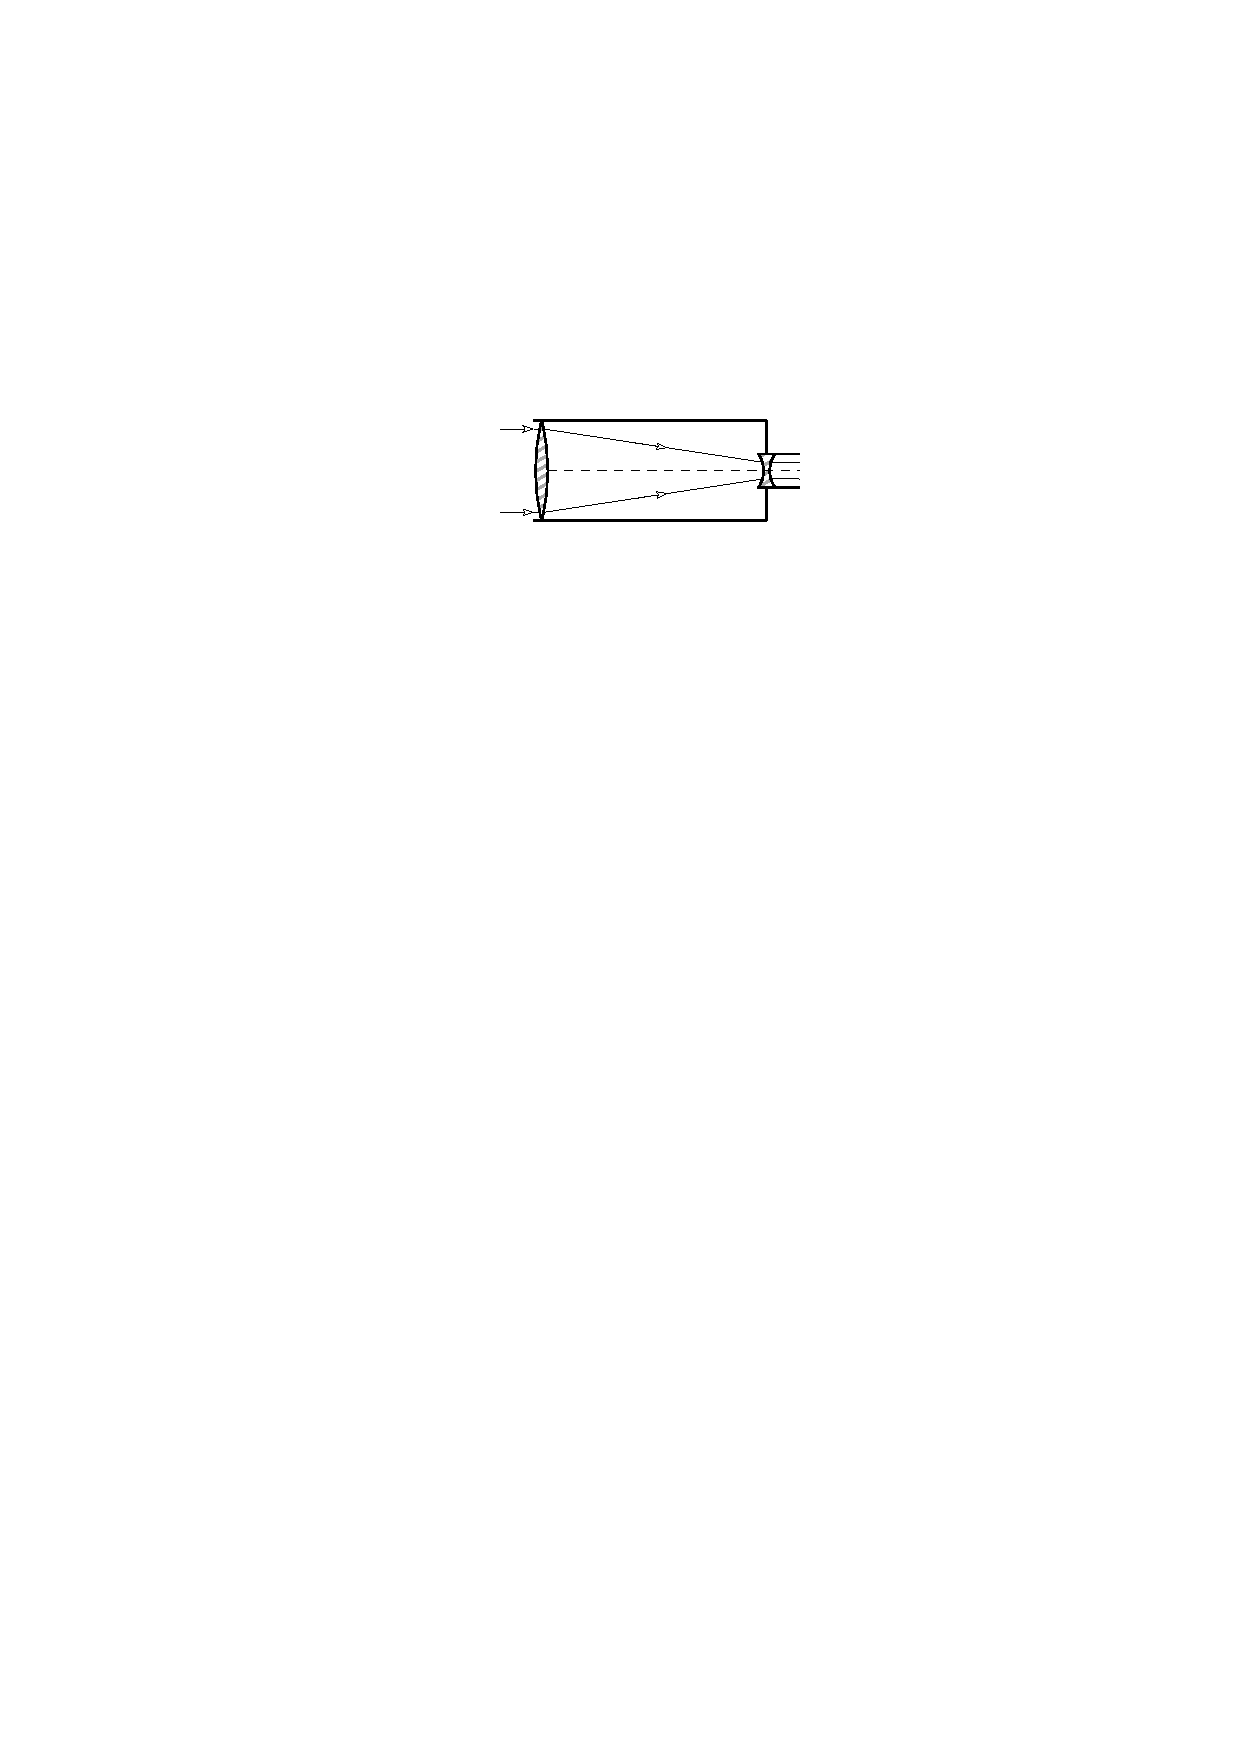
\includegraphics[width = \textwidth]{Galiley}
		\caption{\textit{Рефрактор системы Галилея}}
	 \end{subfigure}
	 \hfill
	\begin{subfigure}{0.49\textwidth}
		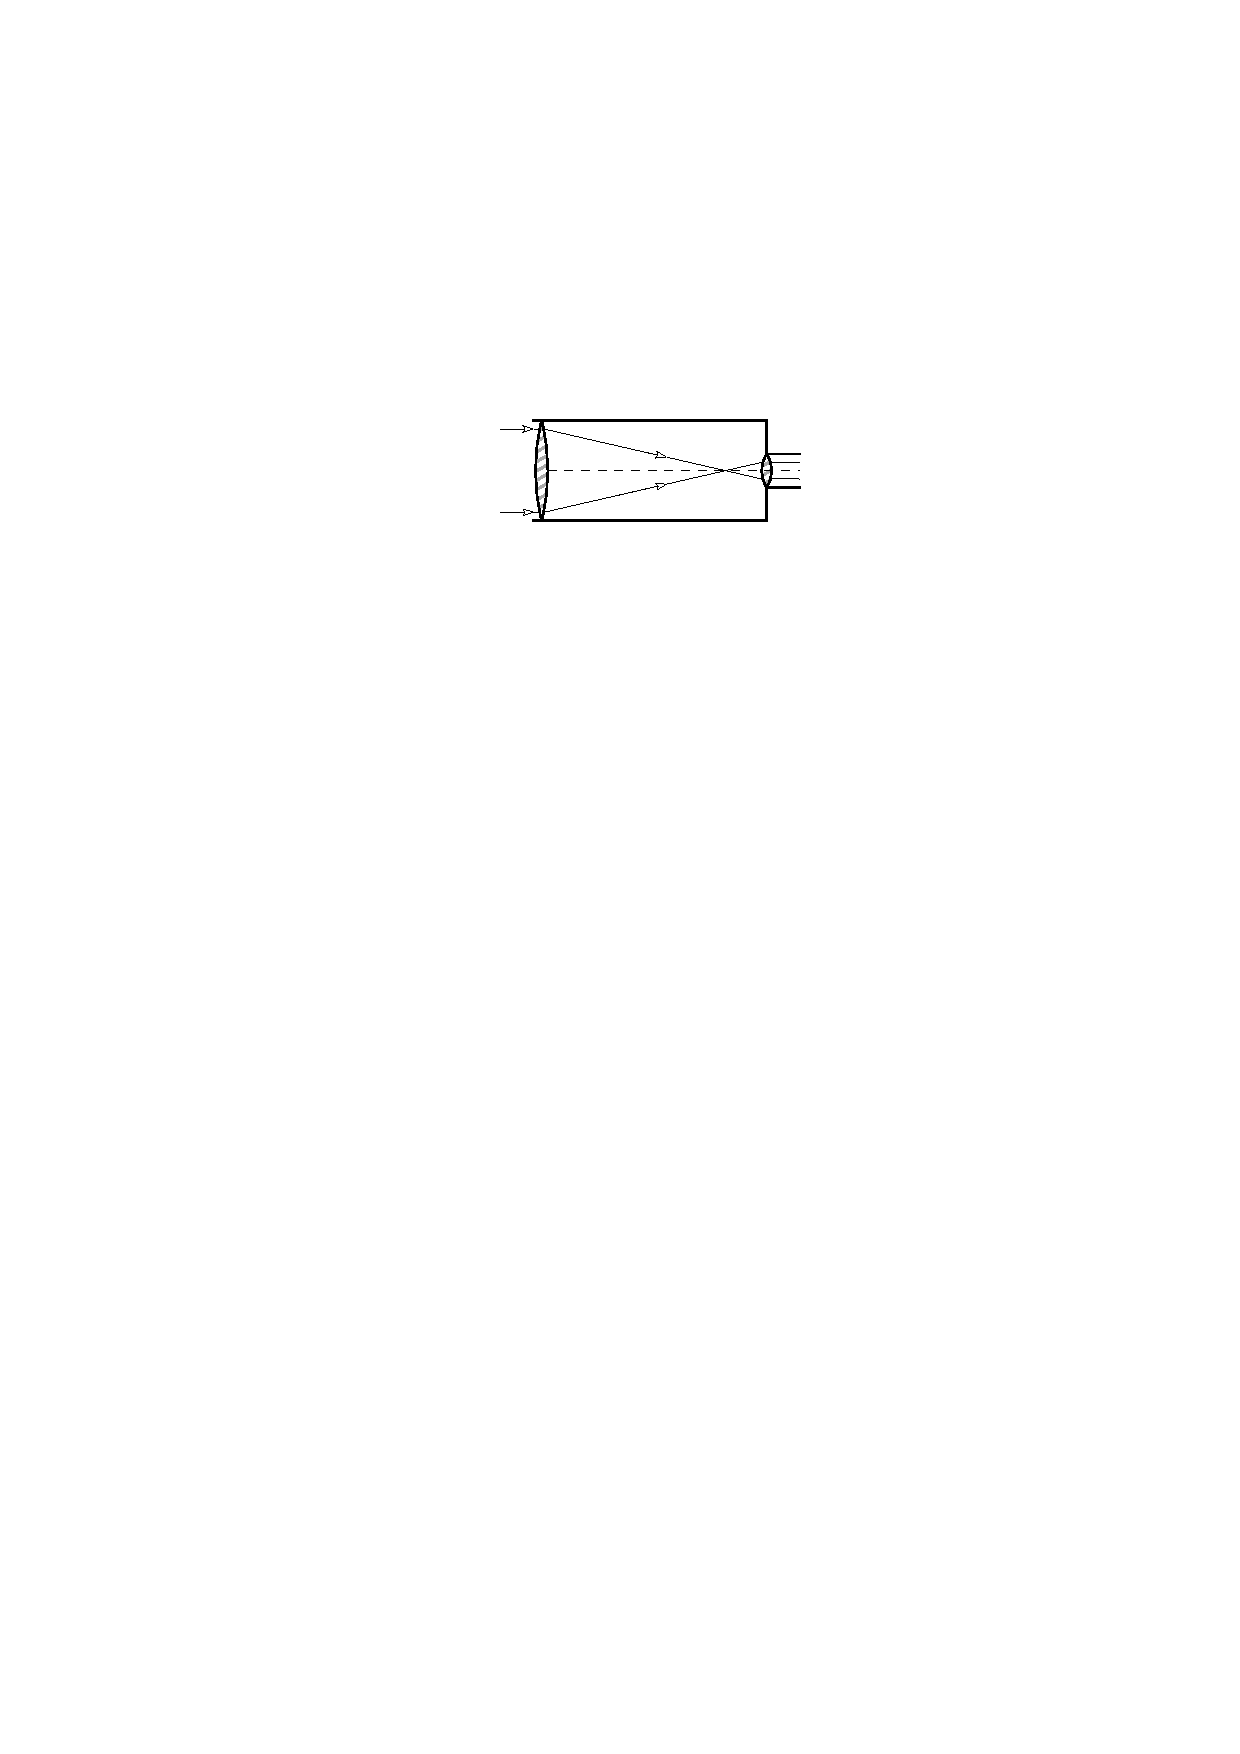
\includegraphics[width = \textwidth]{Kepler}
		\caption{\textit{Рефрактор системы Кеплера} \label{Kepler}}
	 \end{subfigure}
	 
	\begin{subfigure}{0.49\textwidth}
		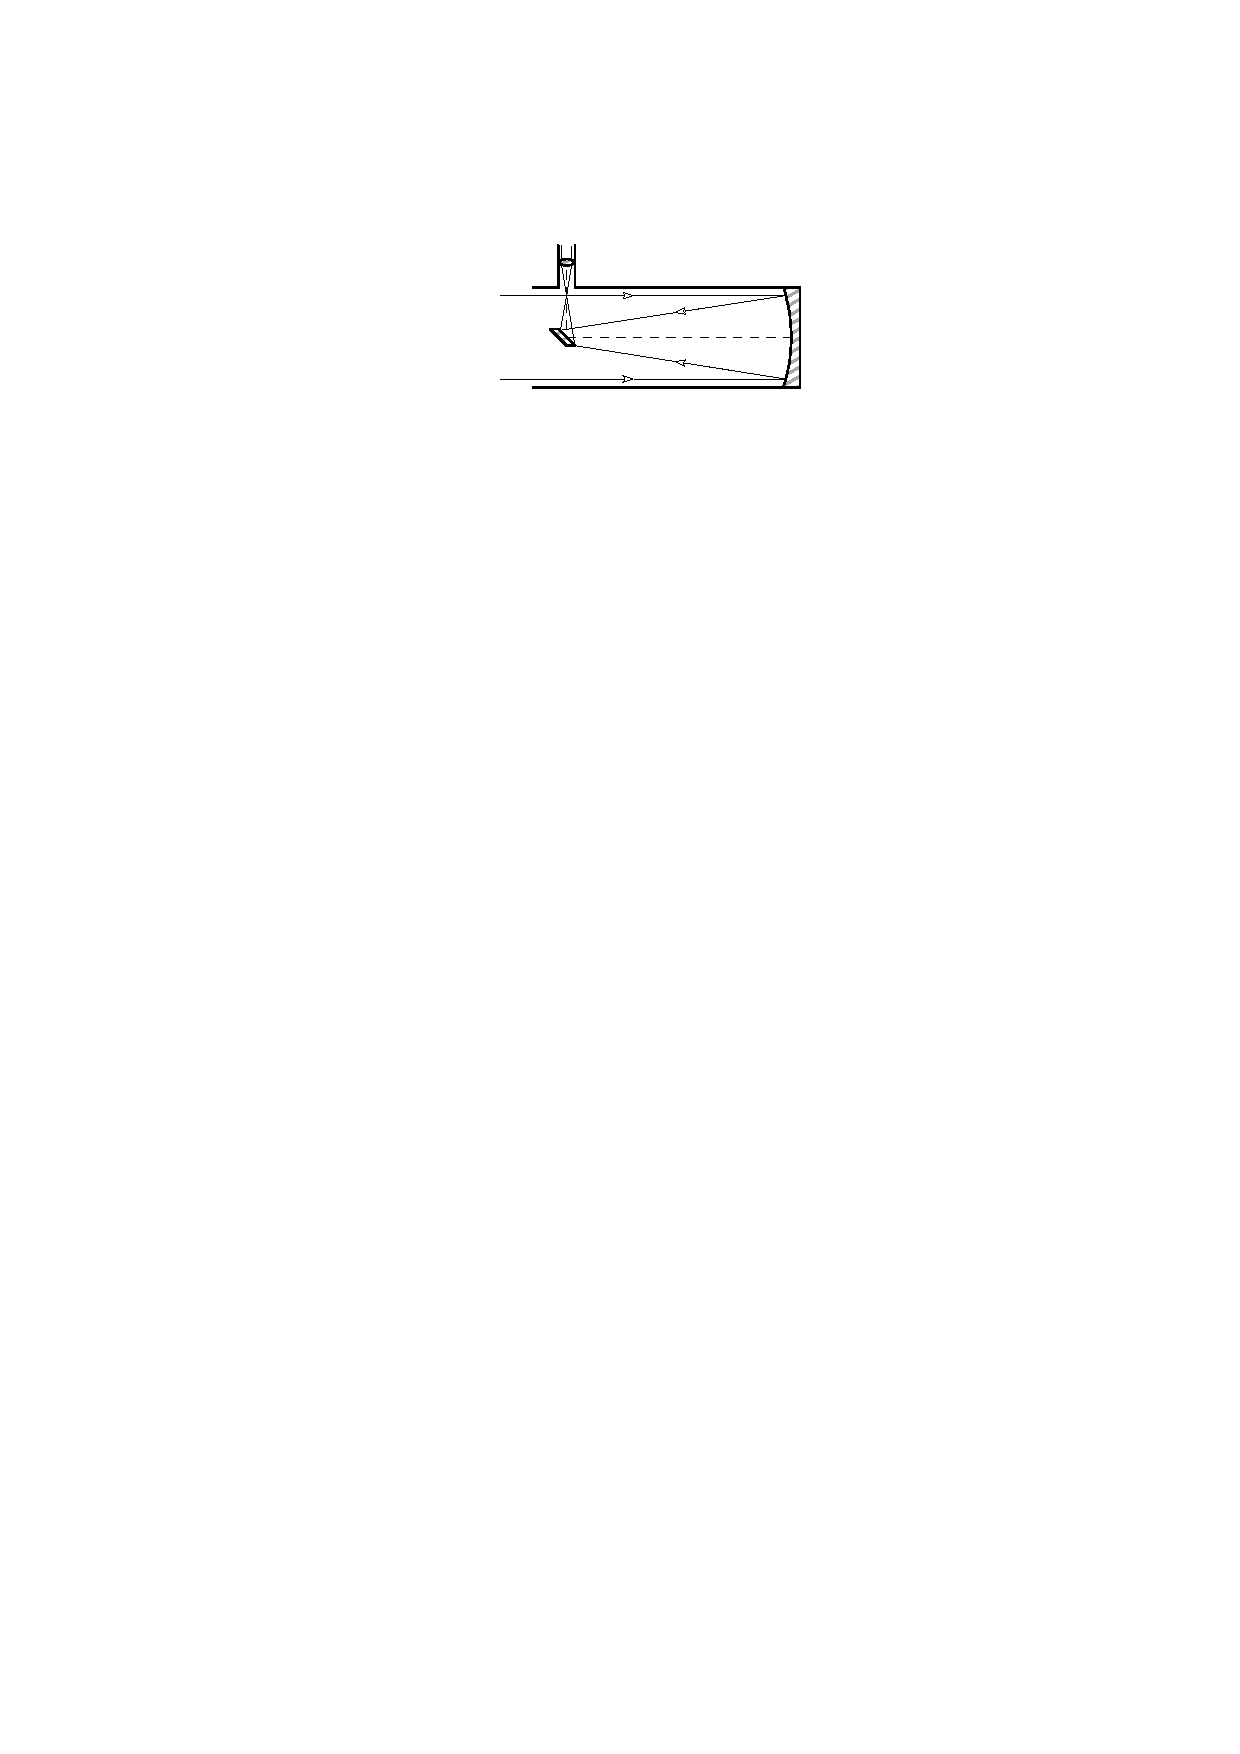
\includegraphics[width = \textwidth]
	{Newton.pdf}
	\caption{\textit{Рефлектор системы Ньютона} \label{Newton}}
	 \end{subfigure}
	 \hfill
	 \begin{subfigure}{0.49\textwidth}
		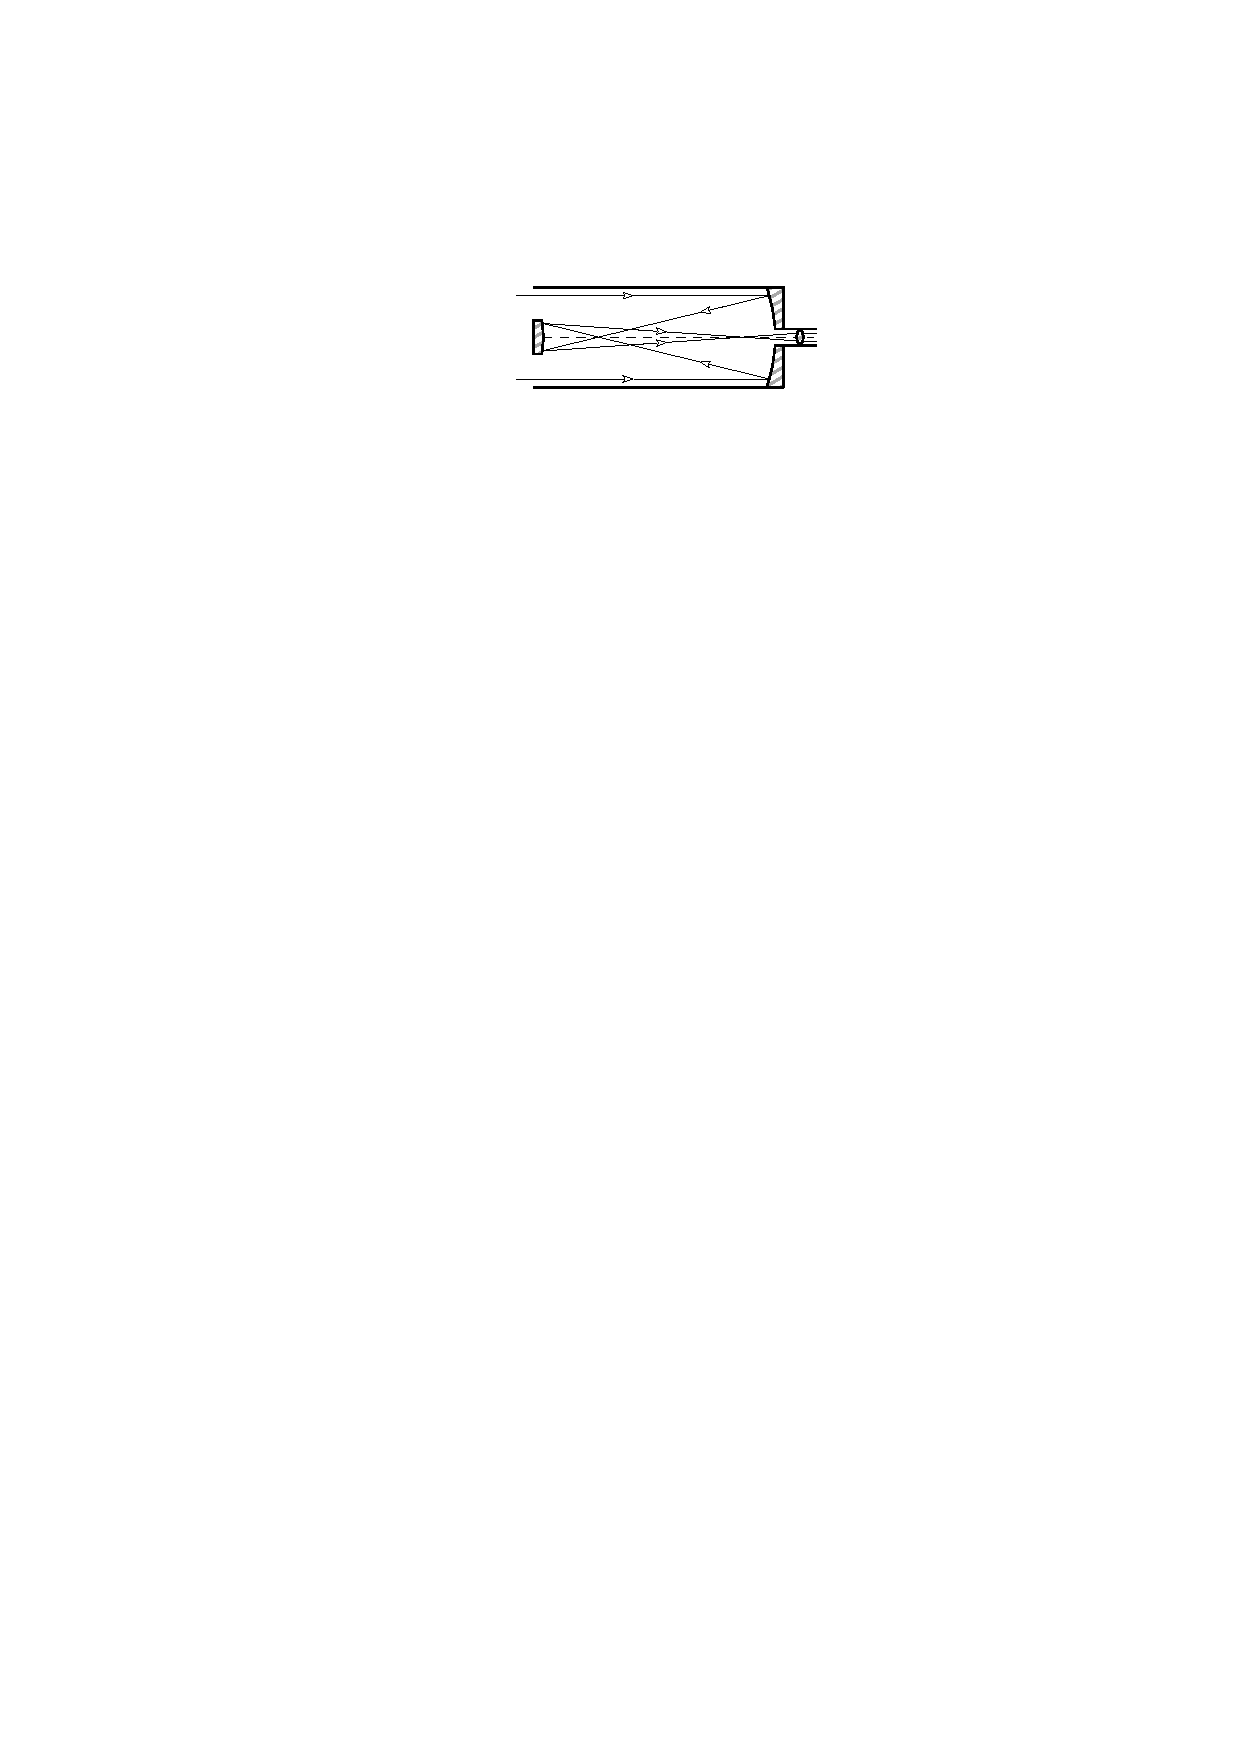
\includegraphics[width = \textwidth]
	{Gregory.pdf}
	\caption{\textit{Рефлектор системы Грегори} \label{Gregory}}
	 \end{subfigure}
	 
	 \begin{subfigure}{0.49\textwidth}
		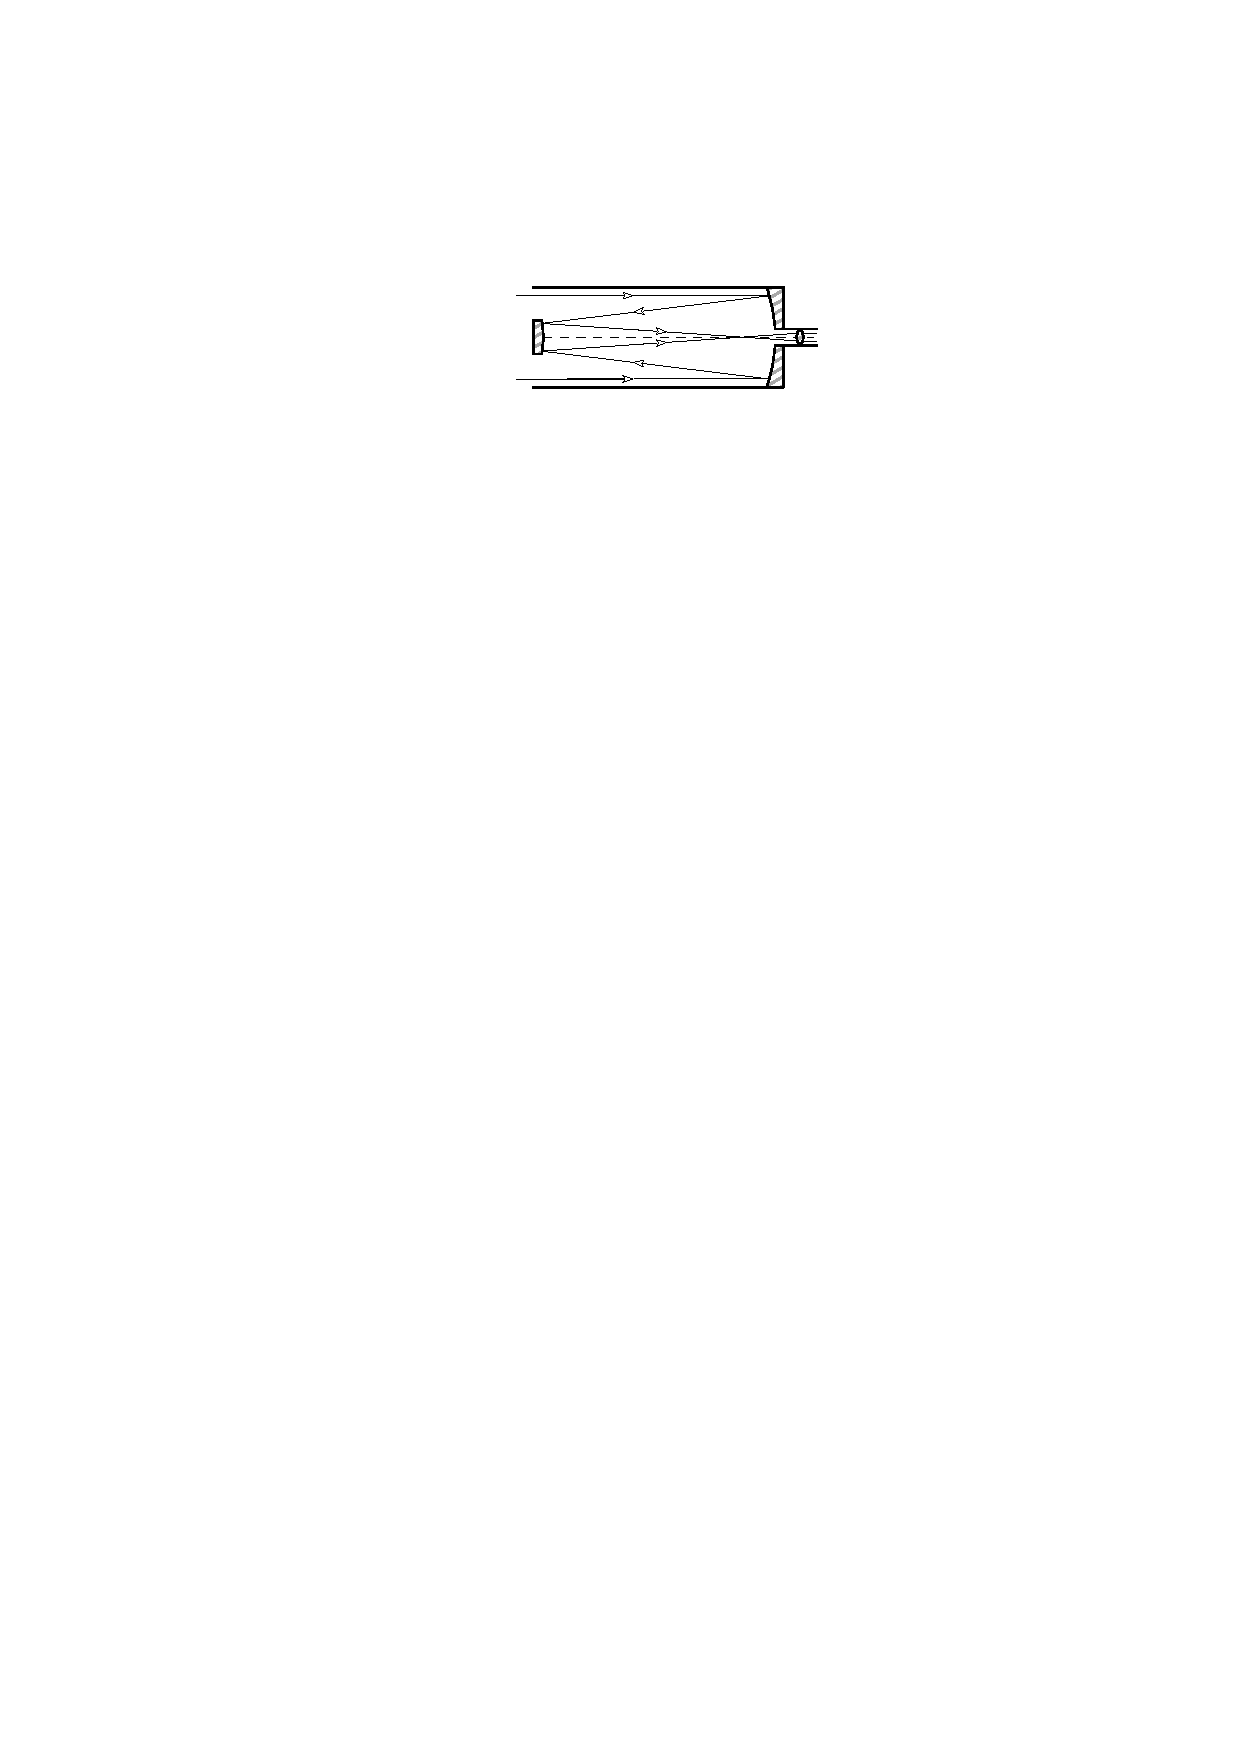
\includegraphics[width = \textwidth]
	{Cassigren.pdf}
	\caption{\textit{Рефлектор системы Кассигрена}}
	 \end{subfigure}
	 \hfill
	 \begin{subfigure}{0.49\textwidth}
		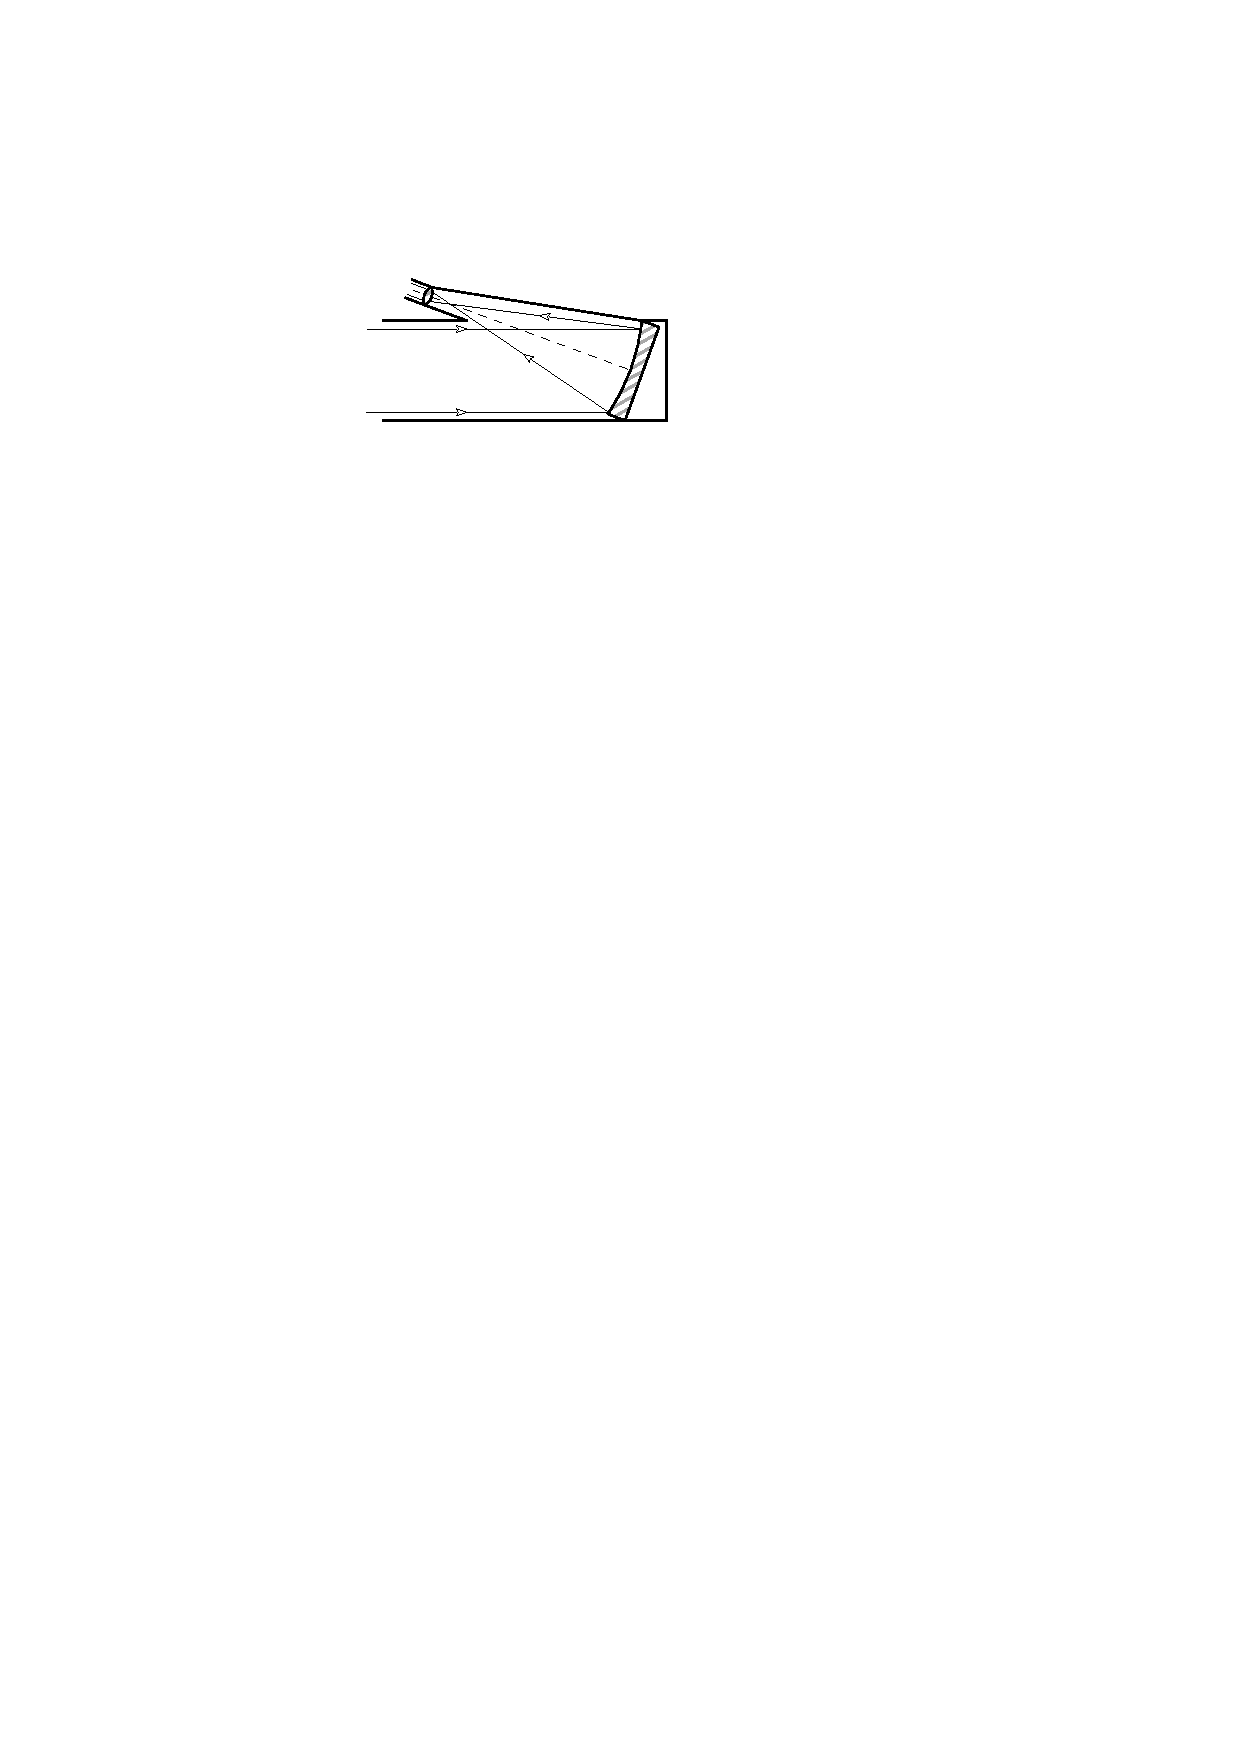
\includegraphics[width = \textwidth]
	{Lomonosov.pdf}
	\caption{\textit{Рефлектор системы Ломоносова}}
	 \end{subfigure}
\end{figure}
\subsection{Монтировки телескопов}
Монтировки телескопов разделяют на 2 основных вида: \imp{экваториальная} и \imp{азимутальная} монтировка (Рис.~\ref{mounts}).
\begin{figure}[h]
	\centering
	\hspace*{.4cm}
	\begin{subfigure}{0.48\textwidth}
		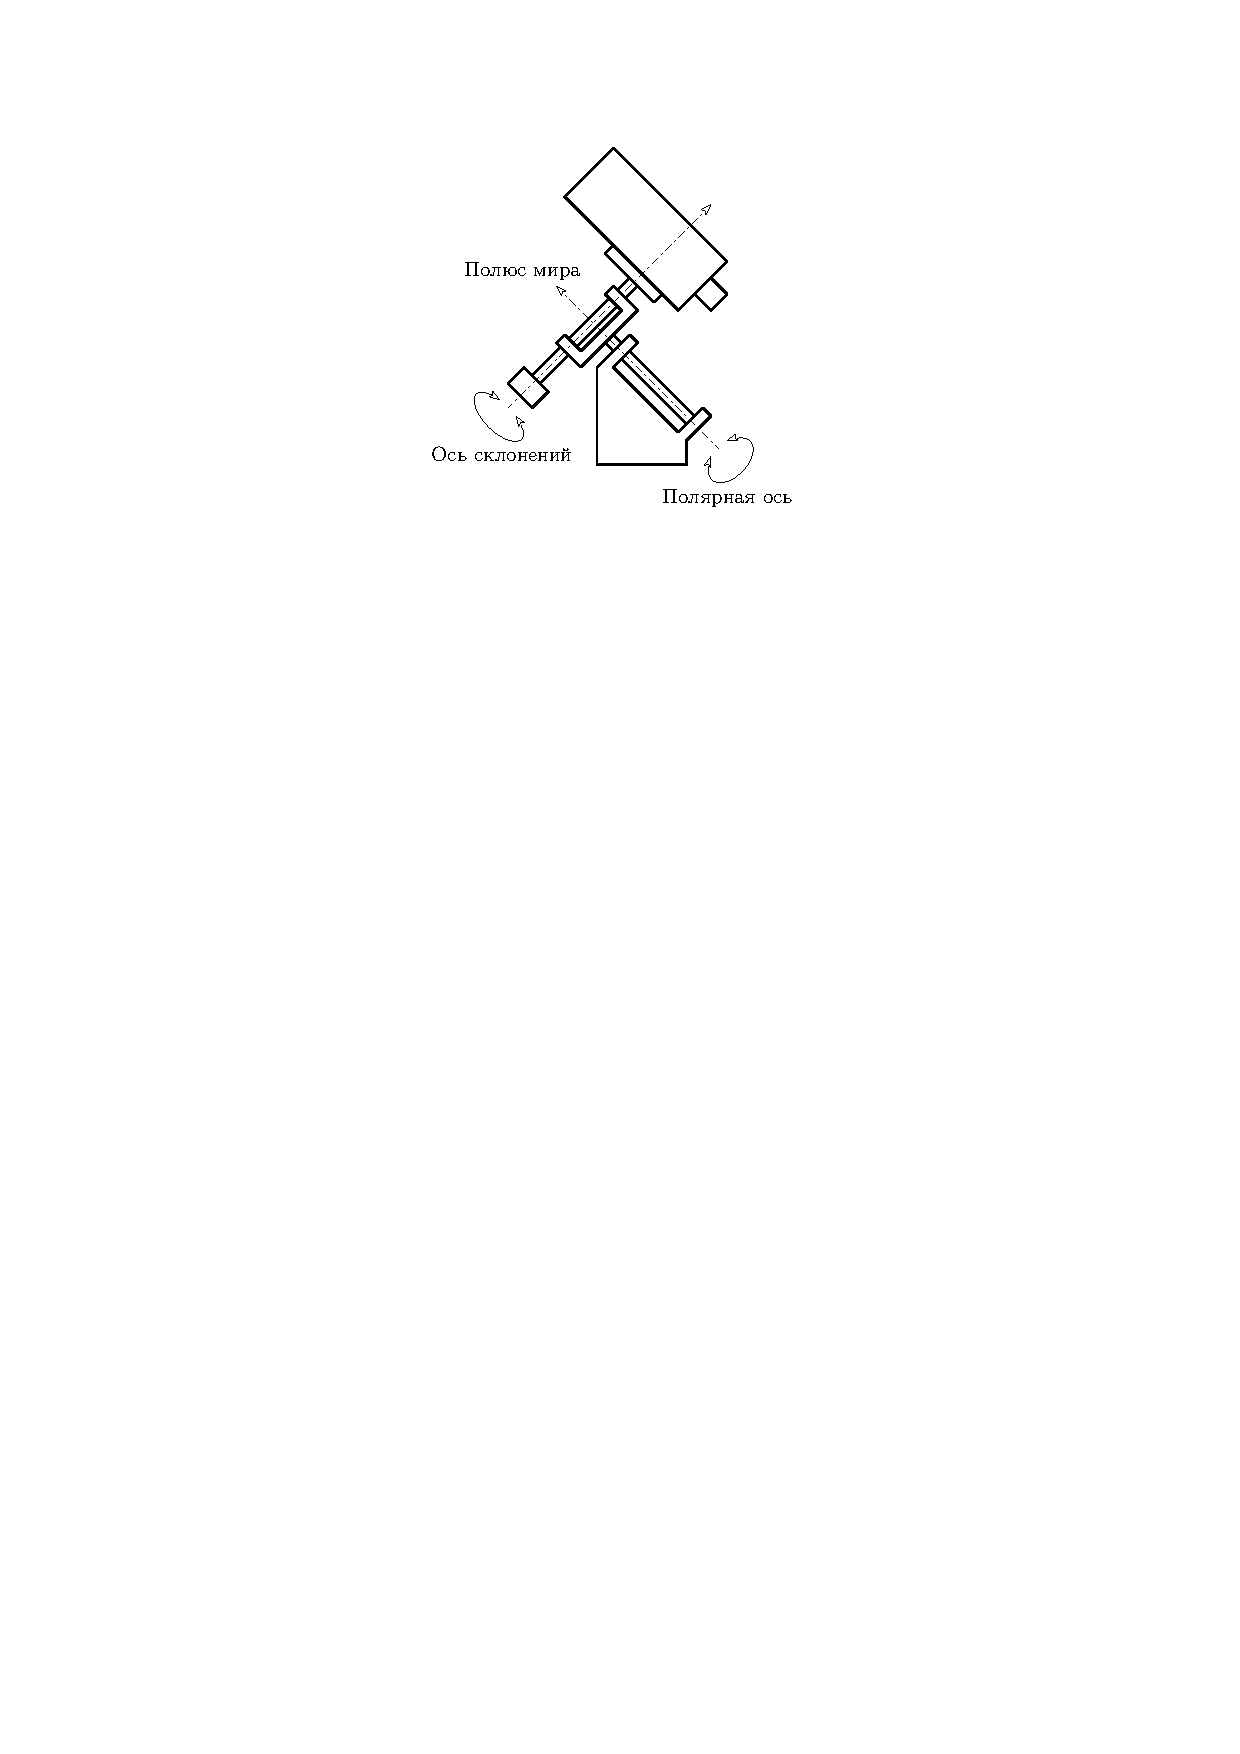
\includegraphics[height = 5cm]{mount-eq}
		\caption{Экваториальная мортировка}
	 \end{subfigure}
	\hspace*{.4cm}
	\begin{subfigure}{0.41\textwidth}
		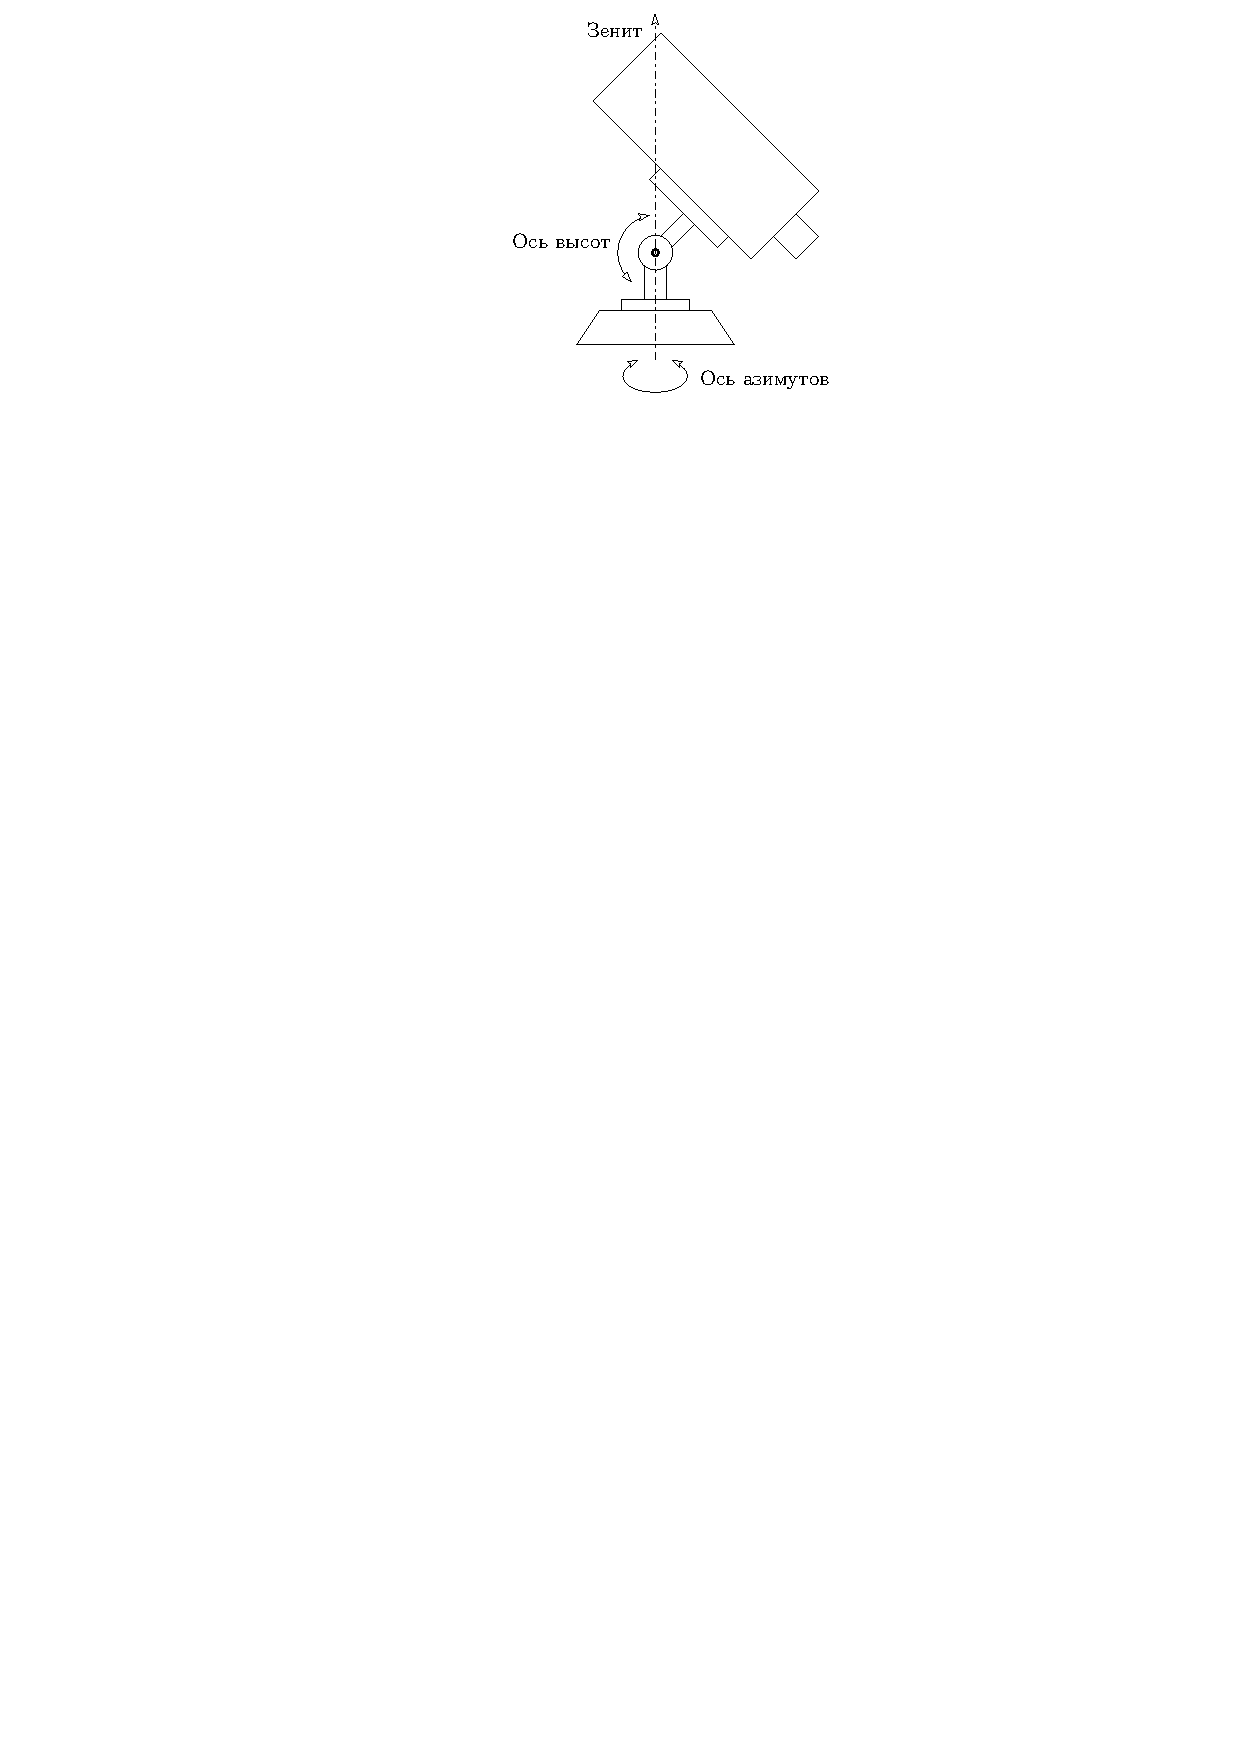
\includegraphics[height = 5cm]{mount-alt}
		\caption{Альтзимутальная монтировка}
	 \end{subfigure}
	 \hspace*{.4cm}
	 \caption{Виды монтировок}
	 \label{mounts}
\end{figure}

\term{Экваториальная монтировка}~--- монтировка, одна ось которой направлена на полюс мира (полярная ось), а другая параллельна небесному экватору (ось склонения). Крупные телескопы обычно устанавливают именно на экваториальные монтировки. Чтобы гидировать с такой монтировкой, нужно поворачивать его с постоянной скоростью вокруг полярной оси в направлении роста часового угла. В свою очередь существуют разновидности экваториальных монтировок: \imp{немецкая}, \imp{английская}, \imp{американская} монтировки и монтировка \imp{с рамой}.

\term{Азимутальная монтировка}~--- монтировка телескопа, имеющая вертикальную и горизонтальную оси вращения, позволяющие поворачивать телескоп по высоте и азимуту. Для слежения за космическими объектами, перемещающиеся по небесной сфере вследствие суточного вращения Земли, телескоп нужно поворачивать одновременно вокруг обеих осей с разными переменными скоростями.
\section{Увеличение и разрешающая способность телескопа}
\textit{Увеличение телескопа} --- это увеличение поля зрения телескопа в определённое количество раз. Увеличение рассчитывается по следующей формуле:
\begin{equation}
\text{Г}=\frac{F}{f}=\frac{D}{d},
\end{equation}
где $F$ --- фокусное расстояние телескопа, $f$ --- фокусное расстояние окуляра, $D$ --- диаметр входного зрачка (телескопа), $d$ --- диаметр выходного зрачка (окуляра).

Также стоит заметить, что диаметры выходного и входного зрачка являются диаметрами пучка света.

Увеличение является \textit{равнозрачковым}, если диаметр выходного зрачка принимается за диаметр зрачка наблюдателя ($d=d_{\text{З}}$):
\begin{equation}
\text{Г}_{\text{Р.З.}}=\frac{D}{d_{\text{З}}},
\end{equation}
где $d_{\text{З}}$ --- диаметр зрачка, обычно в тёмное время суток принимается за 6 мм.

\textit{Разрешающая способность} --- это наименьшее угловое расстояние между двумя объектами, при котором телескоп может различить их раздельно. Разрешние телескопа вычисляется таким образом:
\begin{equation}
\beta=\frac{1.22\lambda}{D},
\end{equation}
где $\lambda$ --- длина волны, при наблюдении глазом $\lambda\approx 550$~нм.
\section{Сферическая астрономия}
\subsection{Изменение экваториальных координт}
\begin{wrapfigure}[12]{r}{0.5\tw}
	\centering
	\vspace{-.7pc}
 	\begin{tikzpicture}
 		\begin{axis}[
 						width	=	.5\tw,
 						height	=	4.5cm,
 						xlabel	=	{Прямое восхождение $\alpha^h$}, 
 						ylabel	=	{Склонение $\delta^{\circ}$},
 						extra y ticks	=	{23.44, -23.44},
 						ytick = {-20, -10, 0, 10, 20},
 						ymax	=	25,
 						ymin	=	-25,
 						xmax	=	24,
 						xmin	=	0,
 						xtick	=	{0, 4, 8, 12, 16, 20, 24}
 					]
 			\addplot [domain=0:24, samples=100] {atan(sin(x*15)*tan(23.44))}; 
 		\end{axis}
 	\end{tikzpicture}
 	\caption{График зависимости склонения от прямого восхождения Солнца}
\end{wrapfigure}
В моменты, когда Солнце находится в \imp{точке весеннего равноденствия}  (20 марта, реже 21) его координаты $\alpha=0^h$, $\delta=0^{\circ}$. Во время прохождения этой точки обе координаты Солнца растут. Так происходит до момента, пока Солнце не пройдет \imp{точку летнегосолнцестояния} (21 июня, реже 20), после этого склонение Солнца начинает уменьшаться. В момент прохождения \imp{точки осеннего равноденствия} (22 или 23 сентября), координаты Солнца составляют $\alpha=12^h$, $\delta=0^{\circ}$. После прохождения \imp{точки зимнего солнцестояния} (22 или 21 декабря) склонение Солнца начинает увеличиваться.

Годичный путь Солнца по небесной сфере можно аппроксимировать синусоидой, откуда очевидным образом получается следующая приближенная формула для расчёта склонения Солнца в заданный момент времени:
\begin{equation}
\delta=\varepsilon\cdot\sin \left(\frac{2 \pi d}{T}\right),
\end{equation}
где $\varepsilon$~--- наклон эклиптики к плоскости небесного экватора, $d$~--- порядковый номер дня после весеннего равноденствия, $T$~--- тропический год.

Более точная формула следует из сферической тригонометрии и имеет вид
\begin{equation}
\delta=\arcsin\left(\sin\varepsilon\cdot\sin \left(\frac{2 \pi d}{T}\right)\right)
\end{equation}

Известно, что движение Солнца по эклиптике происходит неравномерно, поэтому данные формулы не являются верными для точного расчёта.

Прямое восхождение Cолнца связано со склонением данной формулой:
\begin{equation}
\sin\alpha=\frac{\tg\delta}{\tg\varepsilon}
\end{equation}

Большинство формул, представленных выше, следуют из формул перехода между системами координат. 

\section{Солнечное время. Уравнение времени}
\term{Истинные солнечные сутки}~--- промежуток времени между двумя последовательными одноимёнными кульминациями Солнца.

\term{Истинное солнечное время}~--- промежуток времени между нижней кульминацией Солнца и любым другим его положением. Рассчитывается по следующей формуле:
\begin{equation}
T_{\text{ист}}=t_{\text{сол}}+12^h,
\end{equation}
где $t_{\text{сол}}$~--- часовой угол Солнца.

\term{Среднее солнечное время} ($T_m$)~--- промежуток времени между нижней кульминацией среднего Солнца и любым другим его положением. \imp{Среднее Солнце}~--- точка небесной сферы, которая равномерно движется по небесному экватору, совершая полный оборот вокруг точки весеннего равноденствия за тропический год. Зная долготу наблюдателя, нетрудно вычислить среднее солнечное время:
\begin{equation}
T_m=UTC+\lambda,
\end{equation}
где $UTC$~--- всемирное время равное среднему солнечному времени в Гринвиче.

\term{Поясное время}~--- местное среднее солнечное время на срединном меридиане географического часового пояса. В России также установлено декретное время, которое на 1 час больше поясного.


\term{Уравнение времени}~--- разница между истинным солнечным временем и средним солнечным временем:
\begin{equation}
\eta=T_{\text{ист}}-T_m
\end{equation}


\begin{figure}[!h]
\centering
\begin{tikzpicture}
 		 \begin{axis}[width=10cm, height=7cm, no markers, grid = both, xmax = 365, xmin = 0]
  			  \addplot [black, smooth, line width=1pt] table[x=x,y=y]{data/time_eq.txt};
		 \end{axis}
	\end{tikzpicture}
\caption{График уравнения времени}
\end{figure}
\subsection{Рефракция}

\term{Рефракция}~--- преломление в атмосфере световых лучей, исходящих от небесных светил. Для наблюдателя на поверхности планеты с атмосферой положение светила будет отличаться от истинного на некоторый угол. Величина рефракции пропорциональна зенитному расстоянию светила. Средняя величина рефракции у горизонта равна $35'$.

Для зенитного расстояния $z<70$ справедлива формула для величины рефракции:
\begin{equation}
\rho=60.25''\cdot\tg z'\cdot \frac{p}{760}\frac{273^{\circ}}{273^{\circ}+t^{\circ}},
\end{equation}
где $t^{\circ}$~--- температура воздуха, $p$~--- атмосферное давление в мм рт. ст., $z'$~--- видимое зенитное расстояние. При н.у. ($p=760$ мм рт. ст. и $t=0^{\circ}$) формула принимает следующий вид:
\begin{equation}
\rho=60.25''\cdot\tg z'
\end{equation}
\subsection{Сферическая тригонометрия}
Некоторые задачи астрономии, связанные с видимыми положениями небесных тел, сводятся к решениею \term{сферических треугольников}~--- фигур на поверхности сферы, состоящие из трёх точек и трёх дуг больших кругов, соединяющих эти точки.

Свойства сферических треугольников:
\begin{enumerate}
\item Помимо трёх признаков равенства плоских треугольников, для сферических треугольников верен ещё один: два сферических треугольника равны, если их соответствующие углы равны.
\item Два сферических треугольника равны, если они подобны.
\item Для сторон сферического треугольника выполняются 3 неравенства треугольника: каждая сторона меньше суммы двух других сторон и больше их разности.
\item Сумма всех сторон $a+b+c$ всегда меньше $360^{\circ}$.
\item Сумма углов сферического треугольника $s=\alpha +\beta +\gamma$ всегда меньше $540^{\circ}$  и больше $180^{\circ}$
\item Если от двух углов сферического треугольника отнимем третий, получим угол, меньший $180^{\circ}$
\item Площадь сферического треугольника определяется по формуле:
\begin{equation}
s=\sigma\frac{\pi R^2}{180^{\circ}},
\end{equation}
где $\sigma$~--- \term{сферический избыток}, равный разности суммы трёх углов сферического треугольника и $180^{\circ}$.
\end{enumerate}

Возьмём сферический треугольник $ABC$, образованный на сфере радиуса $R$ и с центром в точке $O$. Тогда \term{сферическая теорема} косинусов будет иметь сдедующий вид:


\subsection{Системы небесных координат}
Каждая из систем небесных координат является такой сферической системой координат, в которой радиус не имеет значения, так как параллакс не учитывается и звёзды считаются бесконечно удалёнными от наблюдателя.

\term{Горизонтальная система координат}~--- система координат, в которой основной плоскостью является плоскость математического горизонта, а полюсами~--- зенит и надир~--- точки небесной сферы, расположенные ровно над наблюдателем (зенит) и под ним (надир). Одной координатой является либо \imp{высота} светила $h$ (угловое расстояние между светилом и математическим горизонтом, отсчитываемое в сторону зенита), либо его \imp{зенитное расстояние} $z$ (угловое расстояние между зенитом и светилом). Другой координатой является \imp{астрономический азимут} $A$~--- угол между направлением на юг и направлением на объект, отсчитываемый в сторону запада. $NESW$~--- плоскость математического горизонта, $ZS_*Z'$~--- плоскость суточного движения светила.


\begin{figure}[!h]
\centering
	\begin{subfigure}{0.49\textwidth}
		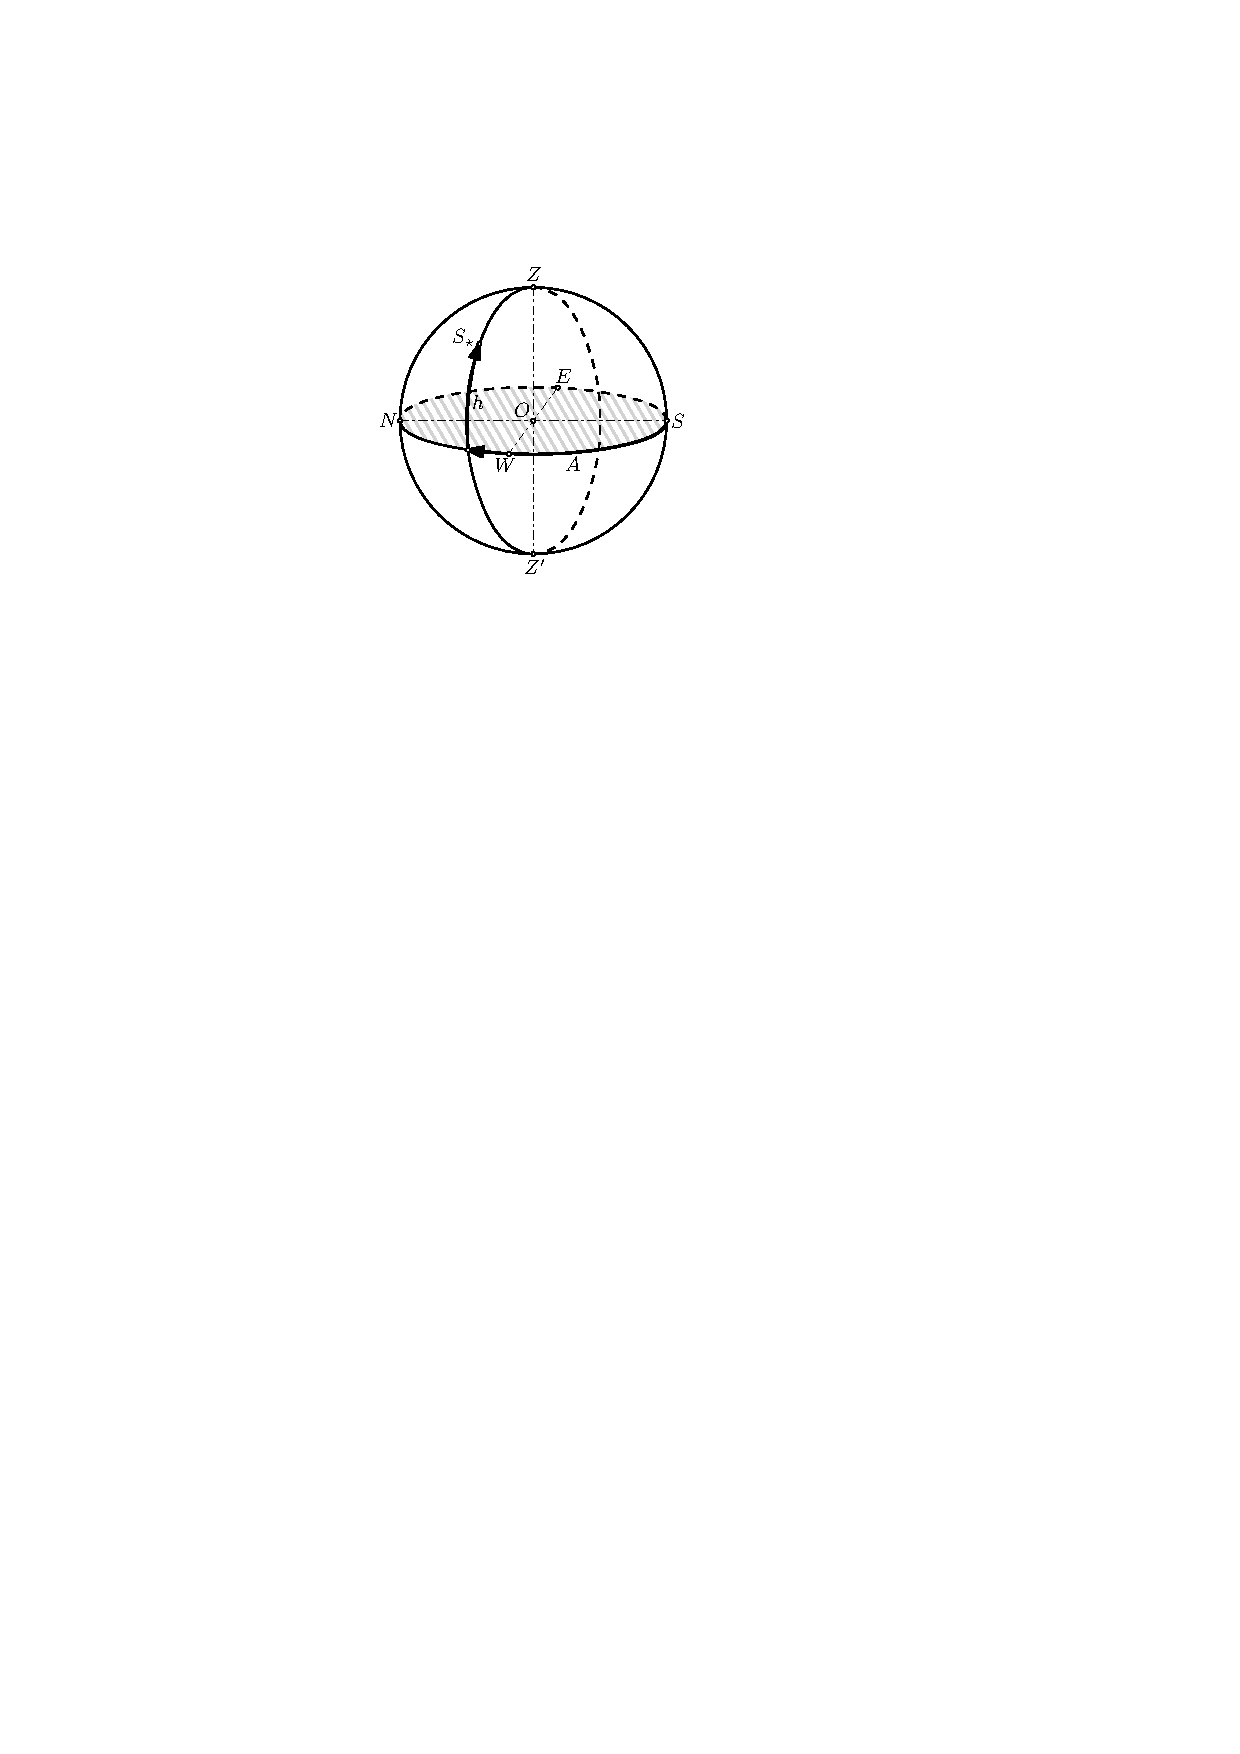
\includegraphics[width = \textwidth]{hor-coordin-sys}
		\caption{Горизонтальная система координат}
	 \end{subfigure}
	 \hfill
	\begin{subfigure}{0.49\textwidth}
		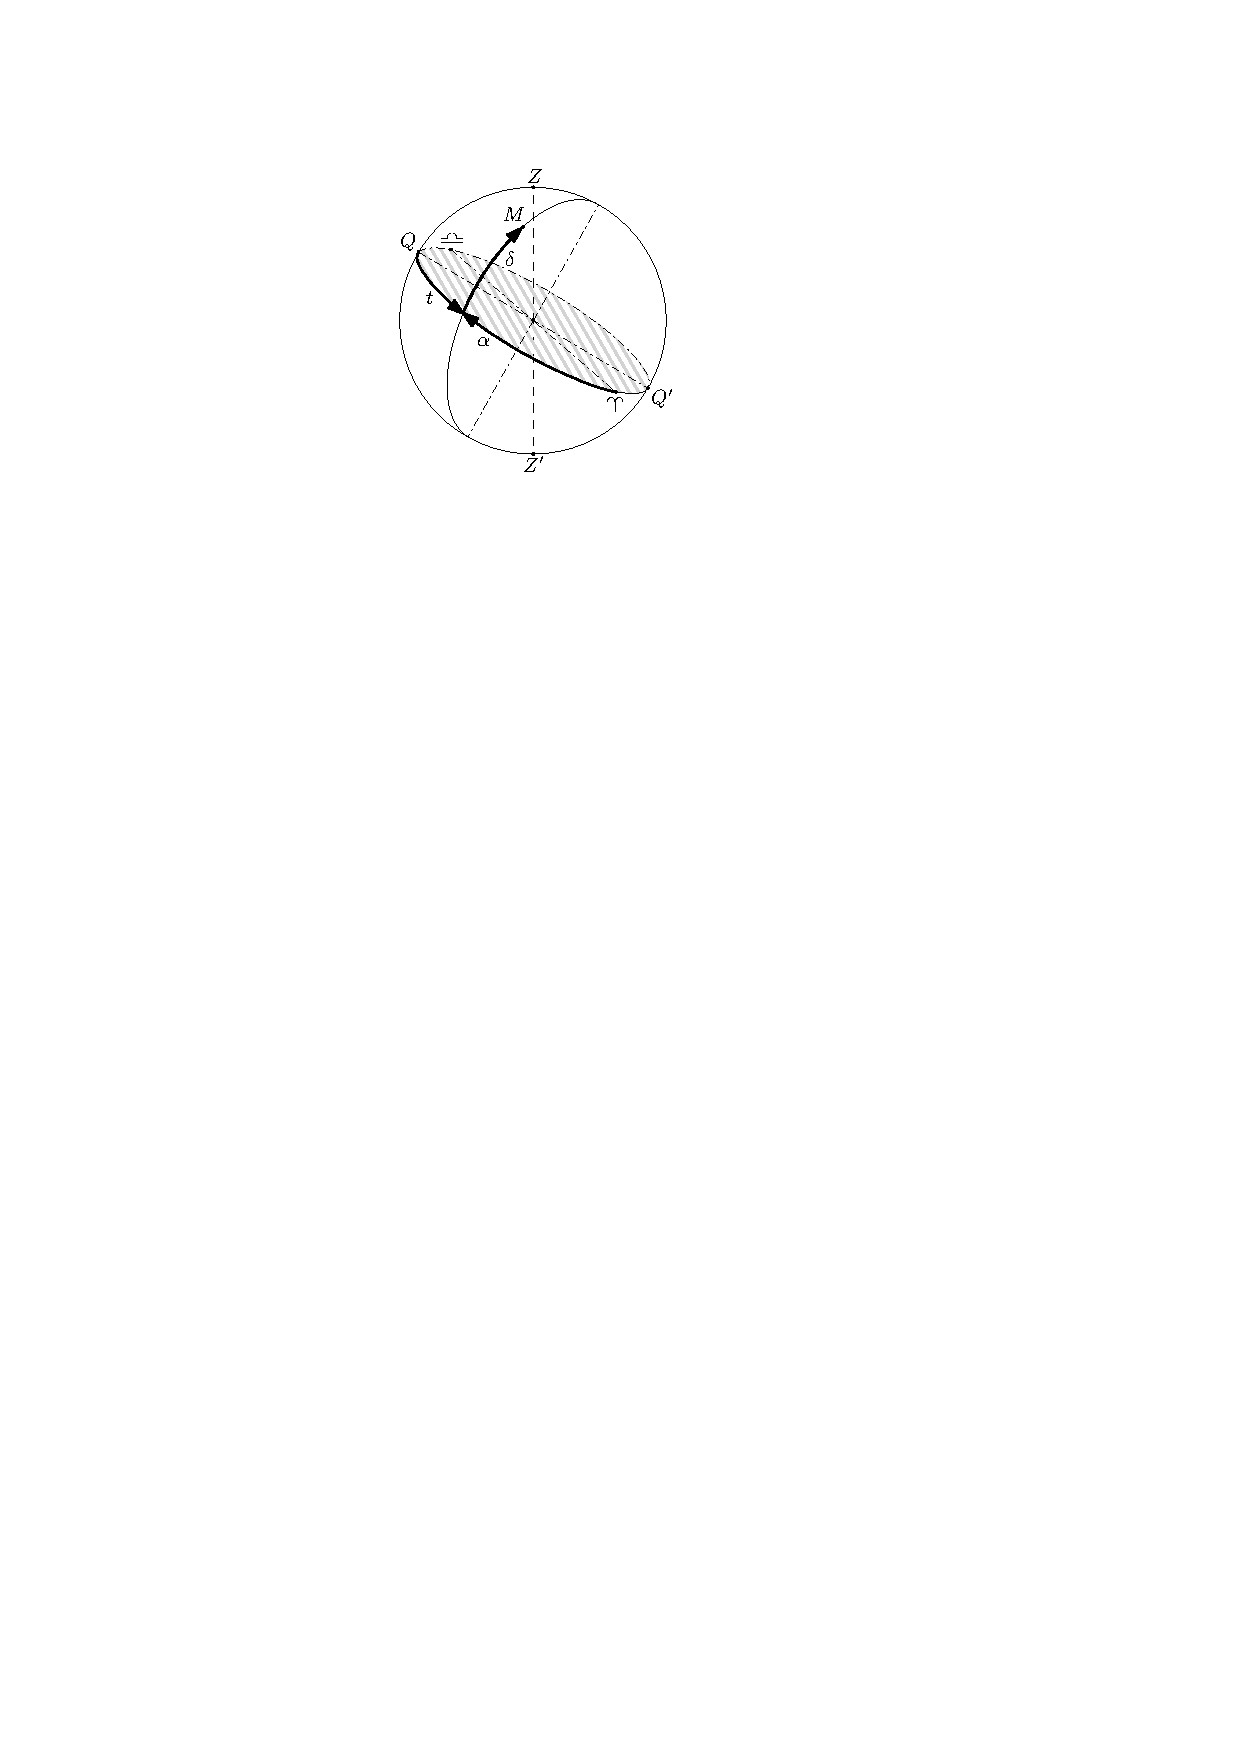
\includegraphics[width = \textwidth]{eq-coordin-sys}
		\caption{Экваториальная система координат}
	 \end{subfigure}
	\caption{Системы координат I}
\end{figure}

\term{Первая экваториальная система координат}~--- система координат, основной плоскостью которой является плоскость небесного экватора $QQ'$. Одной координатой при этом является \imp{склонение} $\delta$~--- угловое расстояние между светилом и плоскостью небесного экватора, отсчитываемое в сторону севера. Иногда вместо склонения используют \imp{полярное расстояние $p$}~--- угловое расстояние между светилом и точкой севера. Другой координатой~--- \term{часовой угол} $t$~--- дуга небесного экватора от верхней точки небесного экватора до круга склонения светила, или двугранный угол между плоскостями небесного меридиана и круга склонения светила. $\aries$ и $\libra$~--- точки весеннего и осеннего равноденствия соответственно. $P_NP_S$~--- ось мира.

\term{Вторая экваториальная система координат}~--- система, основной плоскостью которой является плоскость небесного экватора $QQ'$. Одна координата~--- \imp{склонение} $\delta$. Другой координатой является \imp{прямое восхождение} $\alpha$~--- угловое расстояние между точкой весеннего равноденствия и кругом склонения светила.

\term{Эклиптическая система координат}~--- система координат, основной плоскостью которой является плоскость эклиптики $EE'$. Одной координатой при этом является \imp{эклиптическая широта} $\beta$ (угловое растояние между светилом и эклиптикой, отсчитываемое в сторону северного полюса мира), а другой~--- \imp{эклиптическая долгота} $\lambda$ (угловое расстояние между точкой весеннего равноденствия и кругом эклиптической широты светила).

\begin{figure}[!h]
\centering
	\begin{subfigure}{0.49\textwidth}
		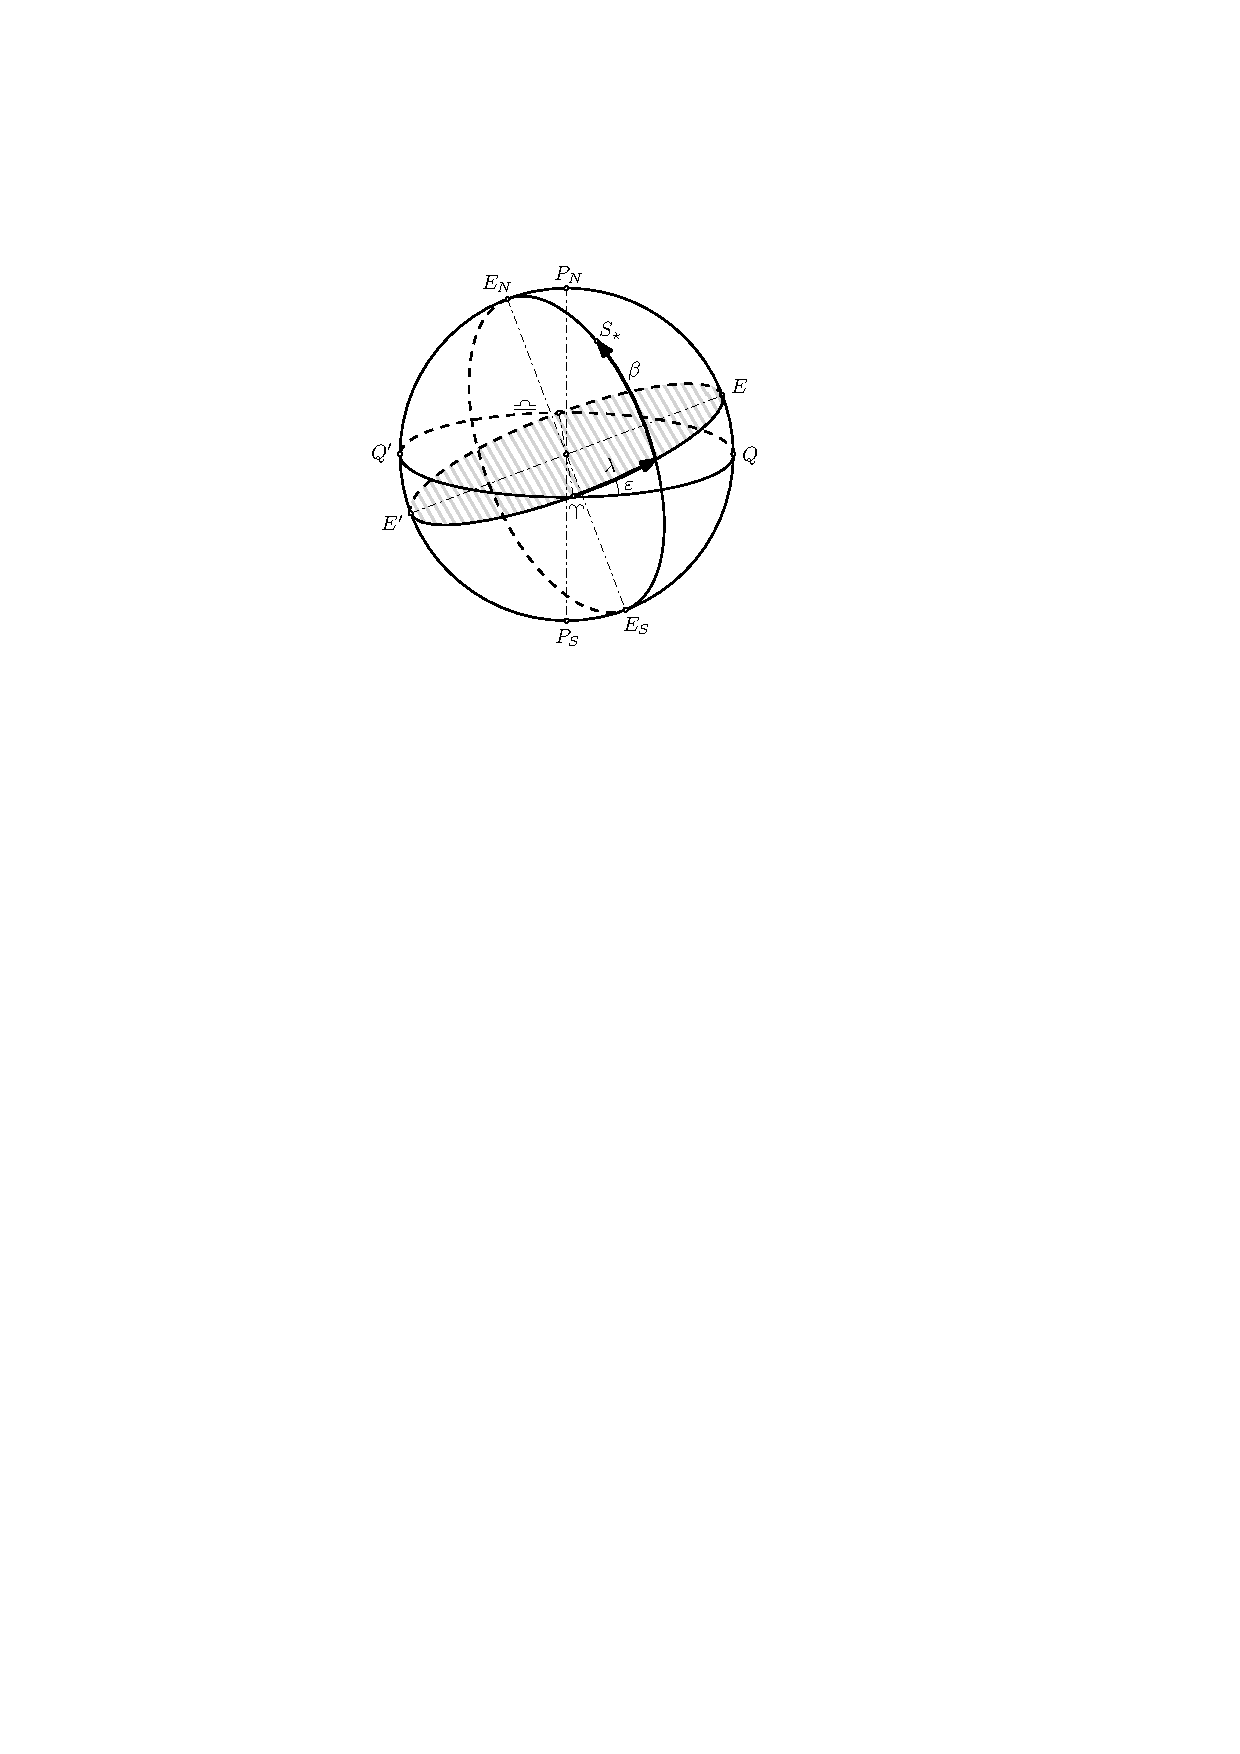
\includegraphics[width = \textwidth]{eql-coordin-sys}
		\caption{Эклиптическая система координат}
	 \end{subfigure}
	 \hfill
	\begin{subfigure}{0.49\textwidth}
		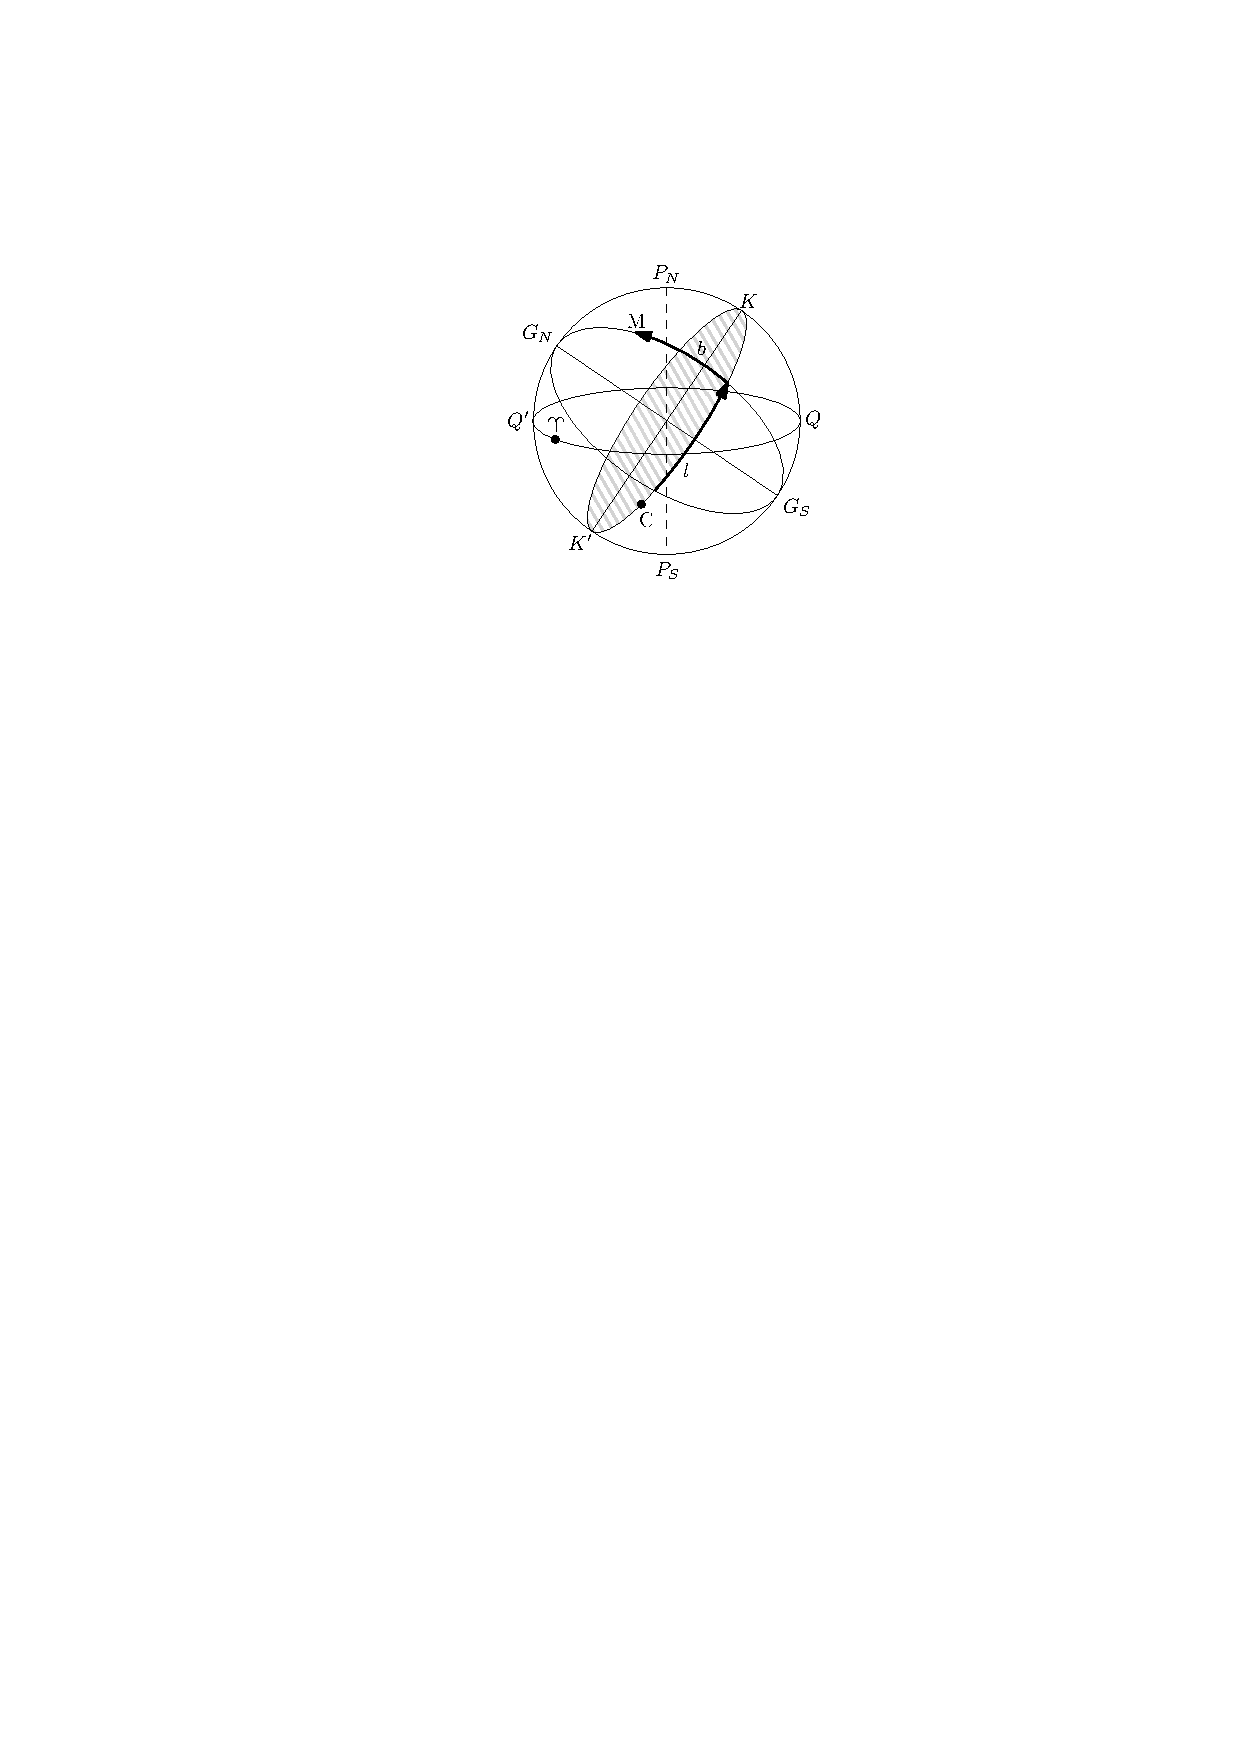
\includegraphics[width = \textwidth]{gal-coordin-sys}
		\caption{Галактическая система координат}
	 \end{subfigure}
	\caption{Системы координат II}
\end{figure}

\term{Галактическая система координат}~--- система координат основной плоскостью которой является плоскость нашей Галактики, которая наклонена к плоскости экватора под углом $62.6^{\circ}$. Одной координатой при этом является \term{галактическая широта} $b$~--- дуга круга галактической широты от эклиптики до светила, или угол между плоскостью галактического экватора и направлением на светило, а другой~--- \term{галактическая долгота} $l$~--- дуга галактического экватора от точки начала отсчёта $C$ до круга галактической широты светила, или угол между направлением на точку начала отсчёта $C$ и плоскостью круга галактической широты светила. Точка $C$ примерно совпадает с направлением на центр галактики и имеет координаты: $\alpha=17^h45.6^m$; $\delta=-28^{\circ}56.2'$ $G_CKK'$~--- плоскость галактического экватора, $G_N$,$G_S$~--- северный и южный полюс галактики.
\section{Объекты космоса}
\subsection{Солнце}
\subsubsection*{Общая информация}

\textit{Солнце} --- центральное тело Солнечной системы. В нём сосредоточено 99,866\%  массы Солнечной системы. Солнце состоит из водорода (73\% от массы), гелия (25\%) и других элементов с меньшим содержанием: железа, никеля, азота, кислорода, кремния, серы, магния, углерода, неона, кальция, хрома и др.

По спектральной классификации Солнце --- звезда типа G2V (жёлтая звезда главной последовательности). Температура поверхности Солнца  примерно $5 800$~К, поэтому Солнце светит почти в белом свете, но прямой свет Солнца у поверхности Земли приобретает жёлтый оттенок из-за рассеяния и поглощения коротковолновой части спектра в атмосфере.

Солнце вырабатывает энергию путём термоядерного синтеза. Каждую секунду в ядре около 4 млн тонн веществе превращается в лучистую энергию.

\subsubsection*{Строение Солнца}

В центре Солнца находится ядро радиусом $150 $ --- $ 180$ тыс. км, в котором идут термоядерные реакции. Плотность  вещества в ядре $1.5\times 10^5~\text{кг}/\text{м}^3$, температура в центре ядра около $1.5\times 10^7$~К.

Над ядром, на расстояниях примерно от 0.2 --- 0.25 до 0.7 радиусов Солнца от его центра, находится зона лучистого переноса. В этой зоне перенос энергии происходит главным образом с помощью  излучения поглощения фотонов. Перепад температур в этой зоне от $2\times10^6$~К сверху до $7\times10^6$~К снизу.

Над зоной \textit{лучистого  переноса} (радиоактивная зона) находится конвективная зона. Этой слой толщиной примерно $2\times10^5$~км, в котором перенос энергии к поверхности совершается движением самого вещества. При приближении к поверхности конвективной зоны температура падает до 5800 К.

\textit{Фотосфера} --- видимая поверхность Солнца, по которой определяется размер Солнца. Эффективная температура фотосферы примерно 5780 К.

\textit{Хромосфера} --- внешняя оболочка Солнца толщиной около 2000 км, окружающая фотосферу. Из хромосферы происходят горячие  выбросы вещества --- \textit{спикулы}. Температура хромосферы увеличивается с высотой до $2\times10^4$~К.

\textit{Солнечная корона} --- последний внешний слой Солнца, который состоит из протуберанцев и энергетических  извержений, образующих солнечный ветер. Средняя температура короны $1-2\times10^6$~К, а в некоторых частях достигает  и $20\times10^6$~К. Столь высокая температура обусловлена процессами, происходящими в магнитном поле звезды. Однако, несмотря на столь высокую температуру, корона видна лишь во время солнечных затмений, так как плотность её очень мала.
  
  
  
\begin{figure}[h!]
\begin{center}
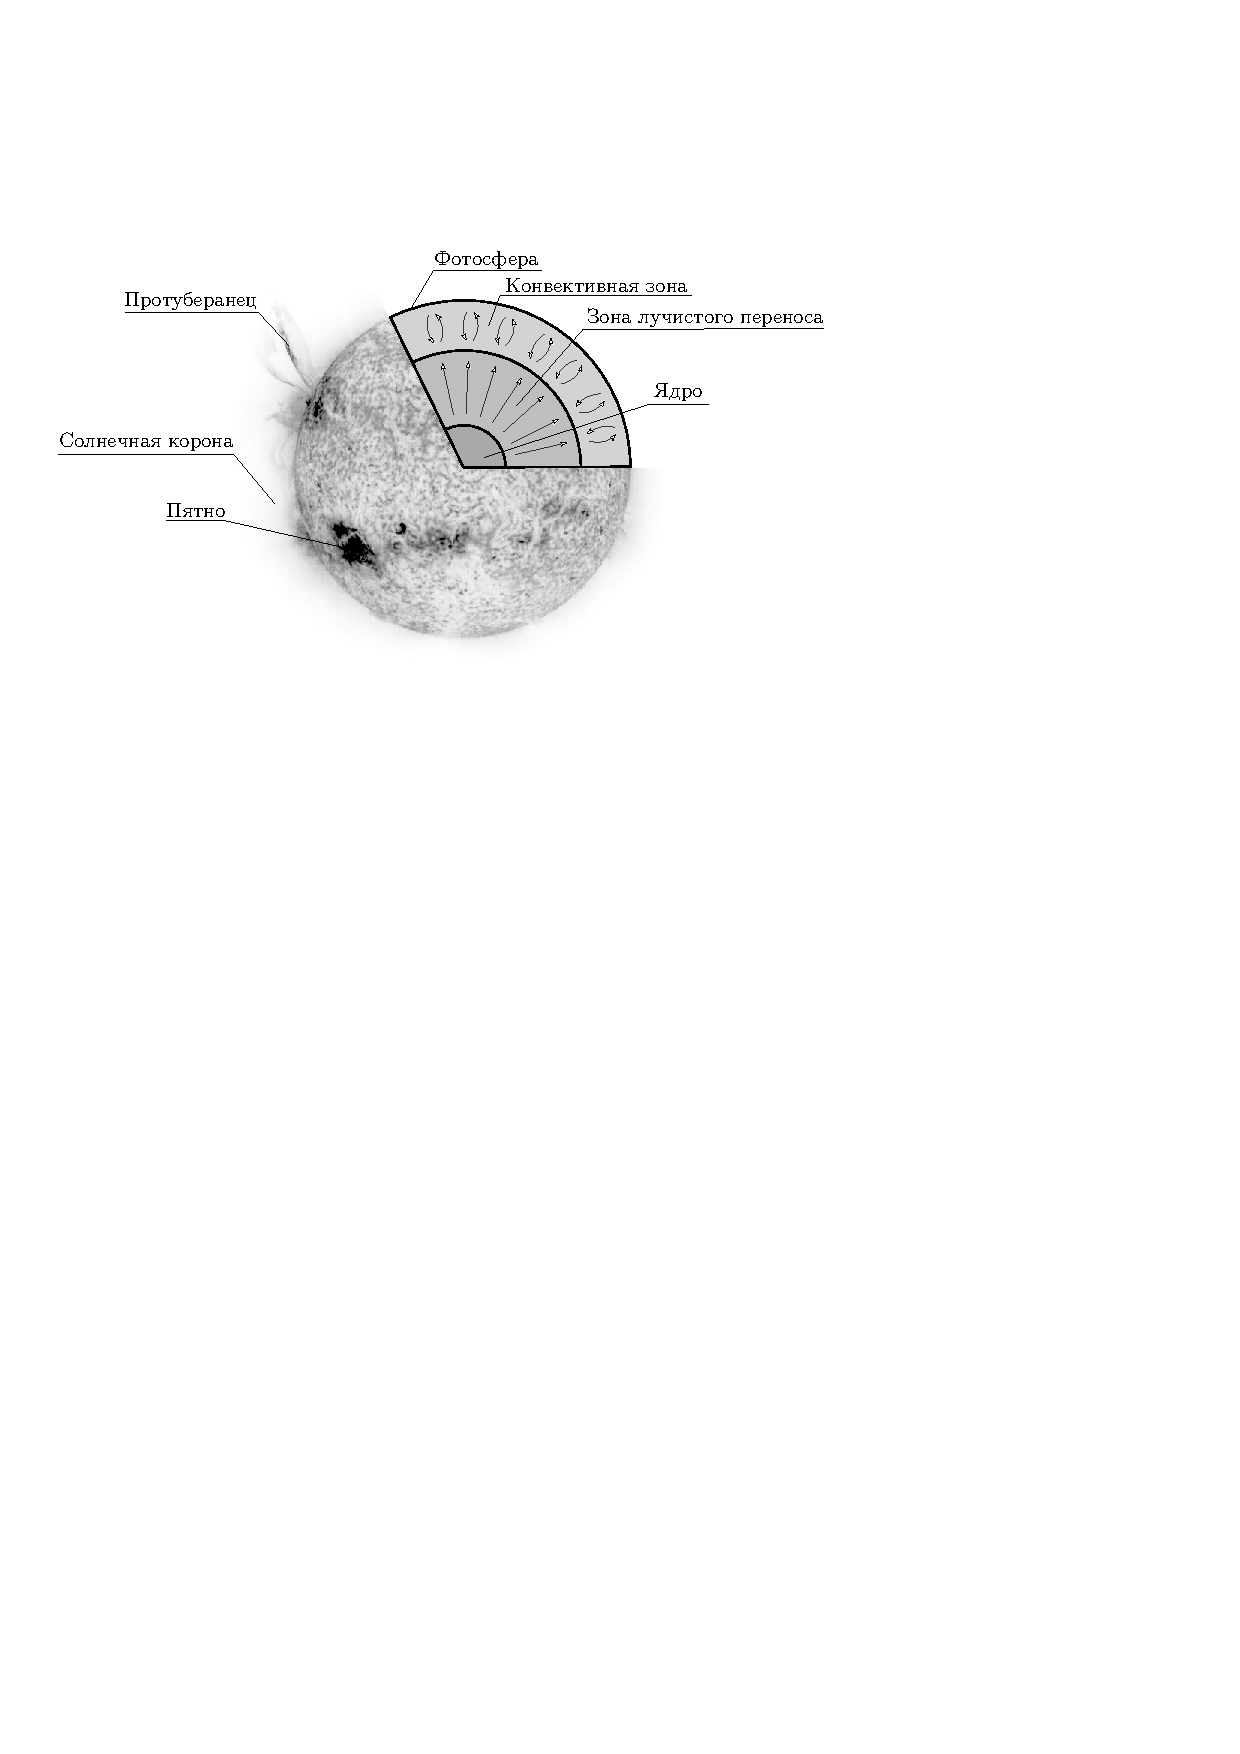
\includegraphics[width=0.65\textwidth]{sun}
\caption{Строение Солнца}
\end{center}
\end{figure}

Солнце вращается не твёрдотельно --- угловая скорость на разных широтах разная, при удалении от экватора она уменьшается. Период обращения Солнца на разных широтах можно найти, наблюдая за солнечными пятнами и другими образованиями. На экваторе период вращения состовляет 25.05 суток, к полюсу он увеличивается до 34 суток. По наблюдениям за пятнами в течение длительного периода при помощи метода наименьших квадратов можно найти зависимость углового перемещения пятна за сутки от гелиографической широты:
\begin{equation}
\Delta\lambda=14.37^{\circ}-2.7^{\circ}\sin^2\varphi,
\end{equation}
где $\Delta\lambda$ --- угловое перемещение пятна, $\varphi$ --- гелиографическая широта.

Вышеприведённая формула верна только для не очень больших значений широт ($\varphi<40^{\circ}$).
\subsection{Спектральные классы звёзд}
\begin{table}[h!]
\centering
\footnotesize
\renewcommand{\arraystretch}{1.4}
\renewcommand{\tabcolsep}{0pt}
\begin{tabularx}{\tw}{|C{0.1}|C{0.3}|C{0.23}|C{0.13}|C{0.13}|C{0.13}|}
\hline
{\bfseries Класс} & {$\mathbf{T}$, К} & {\bfseries Цвет} & {$\mathbf{M}$, $M_{\odot}$} & {$\mathbf{R}$, $R_{\odot}$} & {$\mathbf{L}$, $L_{\odot}$}\\
\hline
O & $3 \times 10^4$ --- $6 \times 10^4$ & Голубой & 60 & 15 & $1.4 \times 10^6$\\

B & $1 \times 10^4$ --- $3 \times 10^4$ & Бело-голубой & 18 & 7 & $2 \times 10^4$\\

A & $7.5 \times 10^3$ --- $1 \times 10^4$ & Белый & 3.1 & 2.1 & 80\\

F & $6 \times 10^3$ --- $7.5 \times 10^3$ & Жёлто-белый & 1.7 & 1.3 & 6\\

G & $5 \times 10^3$ --- $6 \times 10^3$ & Жёлтый & 1.1 & 1.1 & 1.2\\

K & $3.5 \times 10^3$ --- $5 \times 10^3$ & Оранжевый & 0.8 & 0.9 & 0.4\\

M & $2 \times 10^3$ --- $3.5 \times 10^3$ & Красный & 0.3 & 0.4 & 0.04\\
\hline
\end{tabularx}
\caption{Современная спектральная классификация звёзд}
\end{table}

Помимо основных спектральных классов звёзд существуют и дополнительные:
\begin{enumerate}[1)]
\item Класс W --- звёзды Вольфа-Райе, очень тяжёлые яркие звёзды с температурой порядка $70000$~К и интенсивными эмиссиоными линиями спектра.
\item Класс L --- звёзды или коричневые карлики с температурой $1500 - 2000$~К и соединениями металлов в атмосфере.
\item Класс T --- метановые коричневые карлики с температурой $700 - 1500$~К.
\item Класс Y ---  очень холодные (метано-аммиачные) коричневые карлики с температурой ниже $700$~К.
\item Класс C --- углеродные звёзды, гиганты с повышенным содержанием углерода. Ранее относились к классам R и N.
\end{enumerate}

Мнемонические правила для запоминания спектральных классов:
\begin{enumerate}[1)]
\item\textbf{O}h \textbf{B}e \textbf{A} \textbf{F}ine \textbf{G}irl, \textbf{K}iss \textbf{M}e \textbf{R}ight \textbf{N}ow \textbf{S}weetheart.
\item\textbf{W}ell, \textbf{O}nce \textbf{B}ritish \textbf{A}stronomer has \textbf{F}ound \textbf{G}alaxy, \textbf{K}new \textbf{M}ass, \textbf{L}ength, \textbf{T}erm.
\item Вообразите: \textbf{О}дин \textbf{Б}ритый \textbf{А}нгличанин \textbf{Ф}иники \textbf{Ж}евал \textbf{К}ак \textbf{М}орковь --- \textbf{Р}азве \textbf{Н}е \textbf{С}мешно?
\end{enumerate}

\term{Диаграмма Герцшпрунга-Рассела} показывает зависимость между светимостью, спектральным классом и температурой поверхности звезды. 

\begin{figure}
	\centering
%	\begin{tikzpicture}
% 		\begin{axis}[
% 						height	=	12cm,
% 						width	=	10cm,
% 						ymax	=	15.,
% 						ymin	=	-10.,
% 						y dir	=	reverse,
% 						xmax	=	2.,
% 						xmin	=	-.5,
% 						axis x line* = bottom,
% 						axis y line* = right,
% 						xlabel=$B-V$,
% 						y label style = {at={(axis description cs: 1.2, 0.5)}, rotate=180}, 
% 						ylabel	=	{Абсолютная звёздная величина $M$, $~^m$}
% 					]
%%			\addplot+[only marks, mark = o, mark options={scale=0.2, black}] table[x=f, y=m]{data/light-curve-D-Cep.txt};
% 		\end{axis}
% 		\begin{semilogyaxis}[	
% 						height	=	12cm,
% 						width	=	10cm,
% 						ymax	=	8.312e5,
% 						ymin	=	8.312e-5,
% 						xmax	=	2.,
% 						xmin	=	-.5,
% 						minor x tick num = 0,
% 						minor y tick num = 01,
% 						xtick = {-0.264, 0, 0.3, 0.58, 0.791, 1.57},
% 						xticklabels = {B0, A0, F0, G0, K0, M0},
% 						axis x line* = top,
% 						axis y line* = left,
% 						xlabel	=	{Спектральный класс}, 
% 						x label style = {at={(axis description cs: 0.5, 1.11)}, rotate=0},
% 						ylabel	=	{Светимость $L$, $L_\odot$},
% 						ymajorgrids	 =	false,
% 						xmajorgrids	 =	false	
%    				]
%		\end{semilogyaxis}
% 	\end{tikzpicture}
	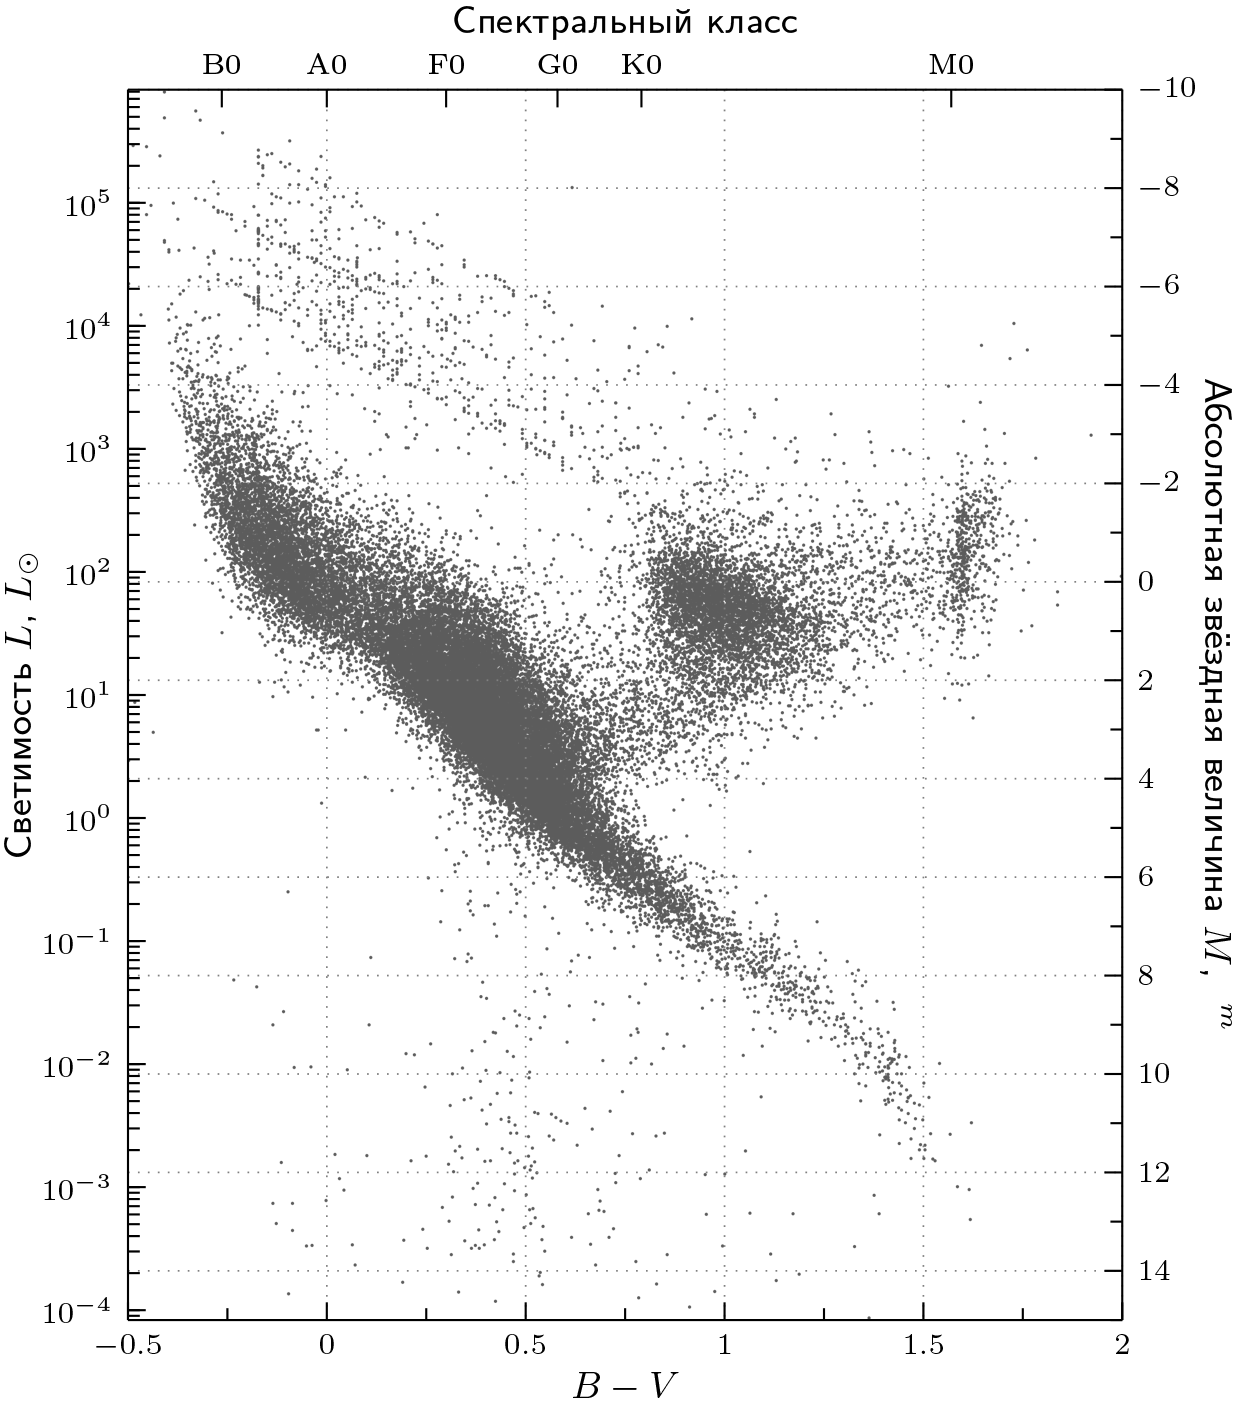
\includegraphics[width=10cm]{gr}
 	\caption{Диаграмма Герцшпрунга--Рассела}
 	\label{pic:d-cep}
\end{figure}


Была предложена примерно в 1910 году независимо Эйнаром Герцшпрунгом и Генри Расселом. Диаграмма используется для классификации звёзд и соответствует современным представлениям о звёздной эволюции.

Около $90 \%$ звёзд находятся на главной последовательности. Их светимость обусловлена термоядерными реакциями превращения водорода в гелий. Выделяется также несколько ветвей проэволюционировавших звёзд --- гигантов, в которых происходит горение гелия и более тяжёлых элементов. В левой нижней части диаграммы находятся полностью проэволюционировавшие белые карлики.


\subsection{Переменные звёзды}
\term{Переменные звёзды}~--- звёзды, у которых наблюдаются колебания блеска.   Для отнесения звезды к разряду переменных достаточно, чтобы блеск звезды хотя бы однажды претерпел изменение.

Переменные звёзды делятся на две большие группы: \imp{затменные} и \imp{физические}, причём физические подразделяются на \imp{пульсирующие} и \imp{эруптивные}.

К \term{пульсирующим} переменным  относят те звёзды, переменность которых вызвана процессами, происходящими в их недрах. Эти процессы приводят к периодическому изменению блеска звезды, а вместе с ним и других характеристик звезды~--- температуры поверхности, радиуса фотосферы и пр. Период переменности заключён в пределе от нескольких долей суток до нескольких лет. Абсолютную звёздную величину  и период связывает следующая формула:
\begin{equation}
	M = -1.01^m - 2.97\lg T,
\end{equation}
где $T$~--- период, выраженный в сутках, а $M$~--- абсолютная звёздная величина.

Классический пример пульсирующих переменных звёзд --- цефеиды.

\begin{figure}[h!]
\begin{center}
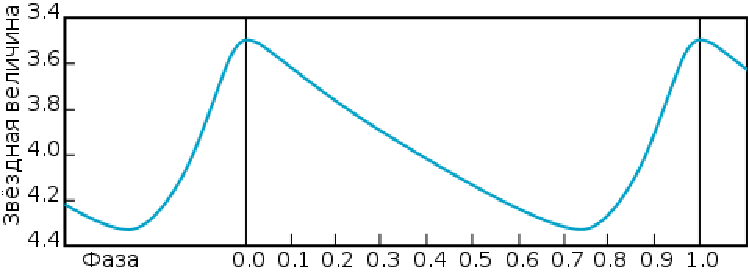
\includegraphics[width=0.7\tw]{var-stars}
\caption{Кривая блеска $\delta$ Цефея}
\end{center}
\end{figure}

К \term{эруптивным} переменным звёздам относятся звёзды, меняющие свой блеск нерегулярно или единожды за время наблюдений. Все изменения блеска эруптивных звёзд связывают с бурными процессами и вспышками в их хромосферах и коронах.

\term{Затменно-переменные} звёзды --- системы из двух звёзд, суммарный блеск которых периодически изменяется с течением времени. Причиной изменения блеска могут быть затмения звёзд друг другом, или изменение их формы взаимной гравитацией в тесных системах.

На всех кривых блеска (Рис.~\ref{var-stars}) заметны два минимума: глубокий (главный), соответствующий затмению главной звезды спутником, и слабый (вторичный), возникающий, когда главная звезда затмевает спутник.

%\begin{figure}[h!]
%	\centering
%	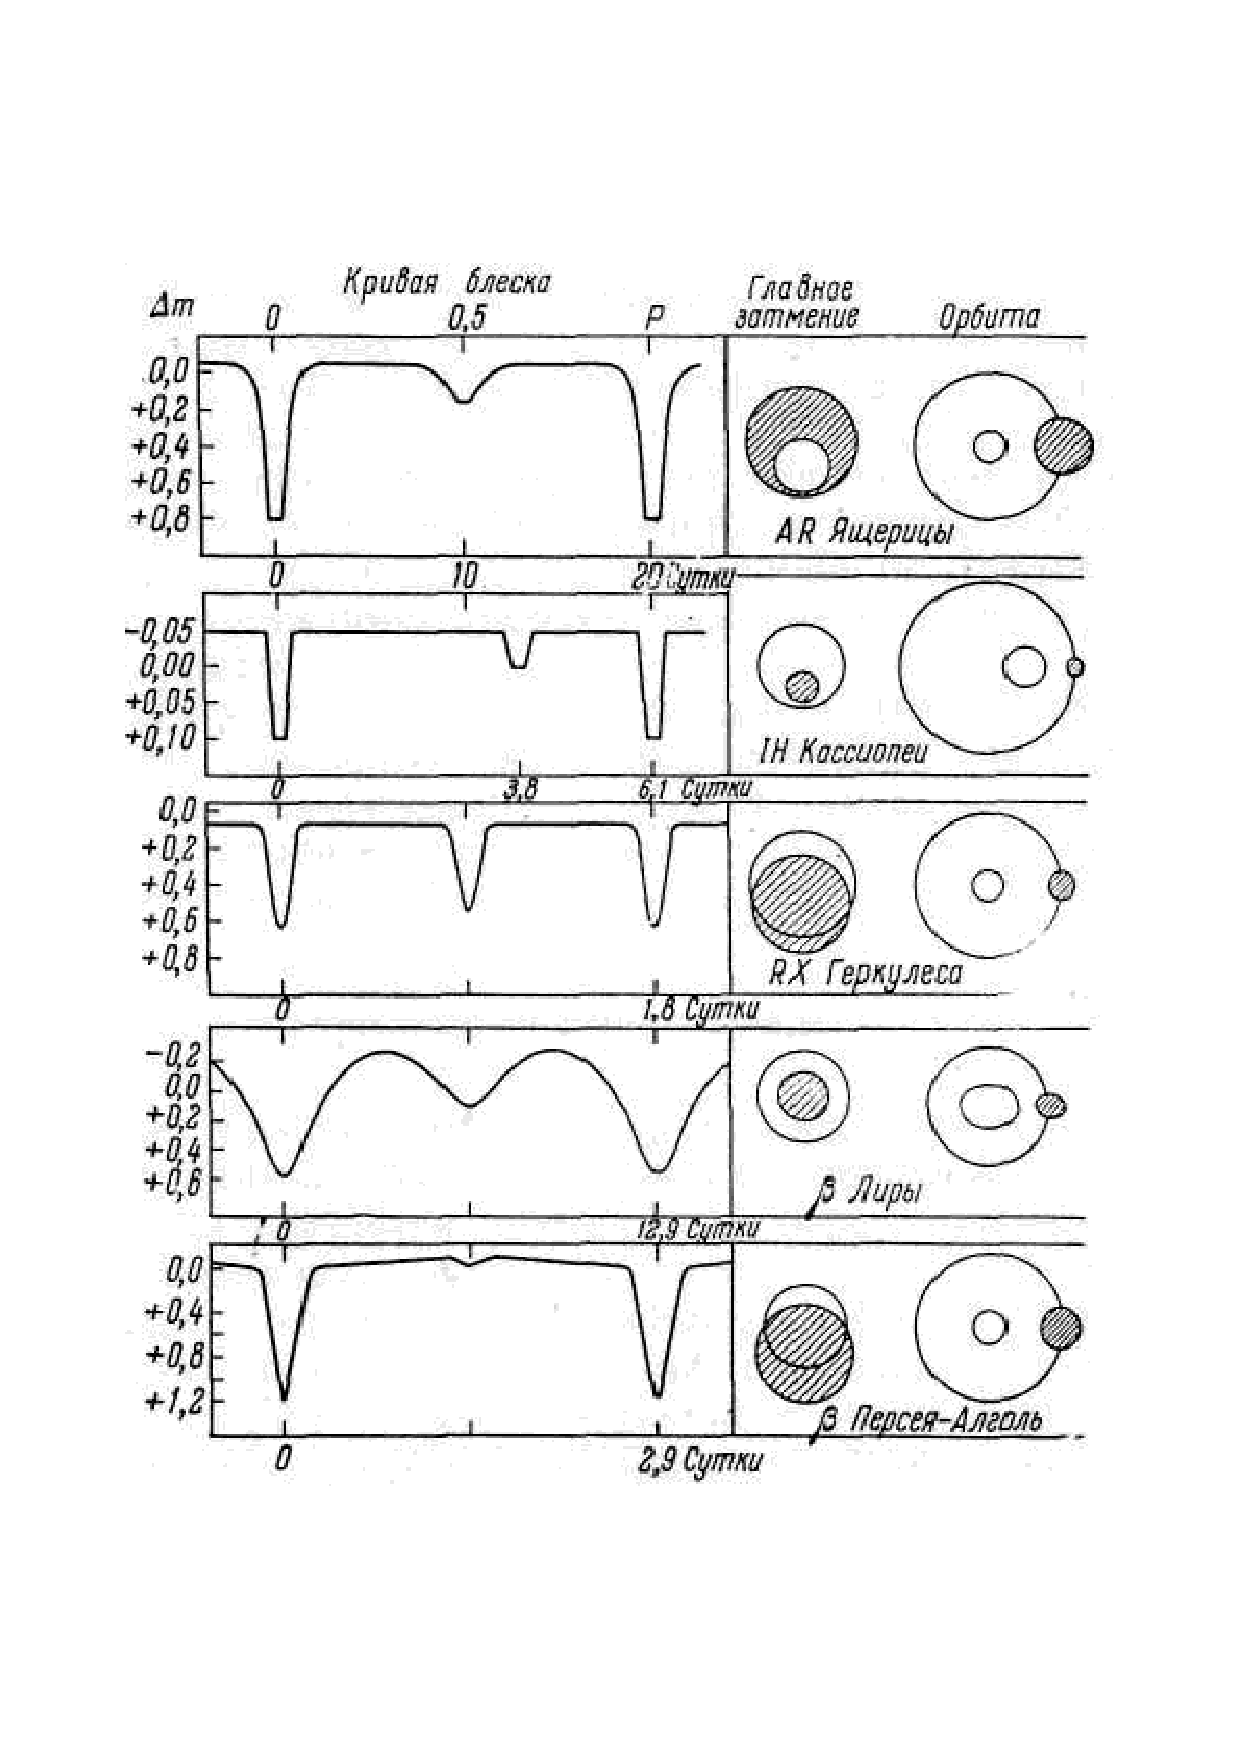
\includegraphics[width=0.8\tw]{var-stars2}
%	\caption{Кривые блеска некоторых затменно-переменных звёзд}
%	\label{var-stars}
%\end{figure}

\begin{figure}[!h]
\centering
 \begin{tikzpicture}
 \begin{axis}[
 no markers,
% xlabel={Прямое восхождение $\alpha^h$}, 
% ylabel={Склонение $\delta^{\circ}$},
 minor x tick num = 1,
 minor y tick num = 1,
 grid = both,
 line width=.7pt, 
% extra y ticks={23.44, -23.44},
 ymax=1.02,
 ymin=0.65,
 xmax=1,
 xmin=0,
% xtick={0,4,8,12,16,20,24}
 ]
% \addplot [domain=0:24, samples=100]{atan(sin(x*15)*tan(23.44))}; 
	\addplot table{data/light-curve-W-UMa.txt};
 \end{axis}
 \end{tikzpicture}
 \caption{График зависимости склонения от прямого восхождения Солнца}
\end{figure}




\subsection{Вырожденные звёзды}
\term{Вырожденные звезды}~--- звезды, в которых силам гравитации противостоят силы давление вырожденного газа. К таким относятся \imp{белые карлики} и \imp{нейтронные звезды}. 

\term{Белые карлики}~--- проэволюционировавшие звёзды лишённые собственных источников термоядерной энергии. 

Масса белого карлика находится в диапазоне от $0.6M_{\odot}$ до $1.44 M_{\odot}$. Верхняя границы массы белого карлика называется пределом Чандрасекара, звезда с массой больше данного предела не может существовать как белый карлик. Радиус белых карликов примерно в $10^2$ раз меньше солнечного, т.е. можно считать, что $R_\text{БК} \simeq R_\oplus$. Плотность белых карликов лежит в диапазоне $10^7$~---~$10^{10}$~$\text{кг}/\text{м}^3$.

\term{Нейтронная звезда}~--- сверхплотная звезда, образующаяся в результате взрыва Сверхновой. Вещество нейтронной звезды состоит в основном из нейтронов. 

Масса нейтронной звезды лежит в пределах от $1.44M_{\odot}$ до $2.5M_{\odot}$ (предел Оппенгеймера-Волкова). Размер данной звезды составляет лишь $10$~--- $20$~км, а плотность составляет $10^{16}$~--- $10^{18}$ $\text{кг}/\text{м}^3$.  Дальнейшему гравитационному сжатию нейтронной звезды препятствует давление ядерной материи, возникающее за счёт взаимодействия нейтронов. Так как нейтронные звёзды образуются в результате  коллапса массивных звёзд, то из-за сохранения момента импульса скорость их вращения очень велика --- максимальная скорость может достигать $10^5$~км/с.
\subsection{Чёрные дыры}
\term{Чёрная дыра}~(ЧД)~--- область пространства-времени с массой $M$, гравитационное притяжение которой настолько велико, что покинуть её не могут даже объекты, движущиеся со скоростью света $c$. Граница этой области называется \imp{горизонтом событий}, а её характерный размер~$R_G$~--- \imp{гравитационным радиусом}, для величины которого справедливо равенство
\begin{equation}
R_G = \frac{2 G M}{c^2}.
\end{equation}

Минимальная масса ЧД составляет около $2.5M_{\odot}$. А плотность ЧД определяется отношением ее массы~$M$ к~объему~$V$, следовательно
\begin{equation}
\rho = \frac{M}{V} = \frac{3c^6}{32\pi M^2G^3}.
\end{equation}

\term{Эффект излучения} (испарения) \term{Хокинга}~--- эффект, при котором гравитационное поле черной дыры поляризует вакуум, в результате чего возможно образование не только виртуальных, но и реальных пар частица~--античастица. Одна из частиц, оказавшаяся чуть ниже горизонта событий, падает внутрь чёрной дыры, а другая, оказавшаяся чуть выше горизонта, улетает, унося энергию (то есть часть массы) чёрной дыры. Для мощности излучения ЧД справедлива формула
\begin{equation}
L = \frac{h c^6}{30720 \pi^2 G^2 M^2},
\end{equation}
где $h$ --- постоянная Планка. Спектр хокинговского излучения для безмассовых полей оказался строго совпадающим с излучением абсолютно чёрного тела, что позволило приписать ЧД температуру, равную
\begin{equation}
T = \frac{h c^3}{16 \pi^2 k G M},
\end{equation}
где $k$ --- постоянная Больцмана.
\subsection{Галактики}
\term{Морфологическая классификация галактик}~--- система разделения галактик на группы по визуальным признакам, используемая в астрономии. Наиболее известной является классификация, разработанная Хабблом и дополненная другими учеными. 
	\begin{figure}[h!]
		\centering
		\vspace{-.9pc}
		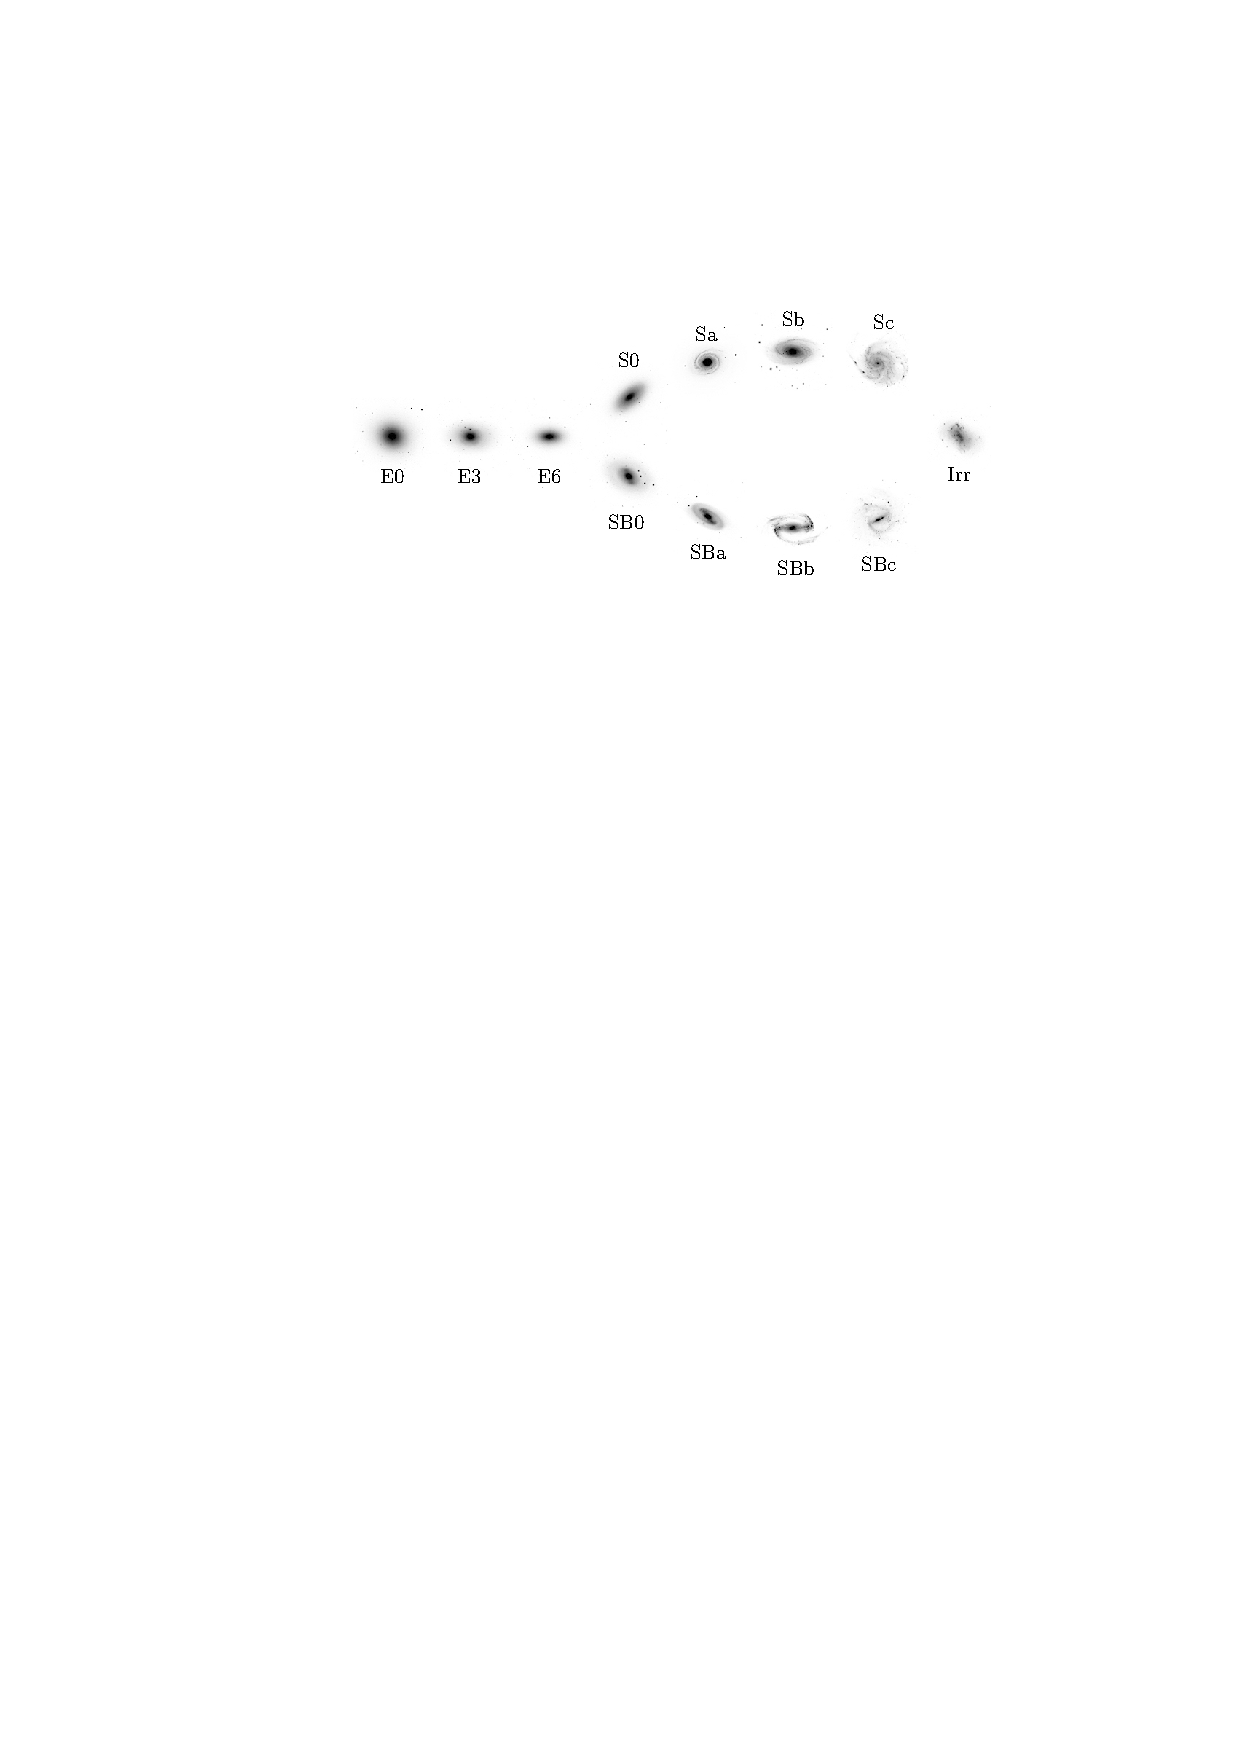
\includegraphics[width=0.65\tw]{hubble-fork.pdf}
		\caption{<<Вилка Хаббла>>}
	\end{figure}
	
Согласно данной классфикации галактики делятся на 4 типа:
\begin{enumerate}[itemsep=3pt, label={\arabic*.}, leftmargin=1pc]
	\item{\term{Эллиптические галактики} имеют гладкую эллиптическую форму без отличительных деталей с равномерным уменьшением яркости от центра к периферии. Обозначаются буквой E с индексом. Индекс можно рассчитать по формуле
		\begin{equation}
		i = 10 \cdot \left(1 - \frac{b}{a}\right),
		\end{equation}\nopagebreak
		где $a$ и $b$~--- большая и малая полуоси видимого эллипса. 
		
		К линзовидным галактикам с абсолютной звёздной величиной около $-21^m$ применимо соотношение Фабер-Джексона:
		\begin{equation}
			L \propto \sigma^4,
		\end{equation}
		где $\sigma$~--- дисперсия скоростей вещества в галактике.}
	\item{\term{Спиральные галактики} состоят из уплощенного диска из звезд и газа, в центре которого находится сферическое уплотнение, называемое балджем, а также обширного сферического гало. Спиральные галактики обозначаются SB при наличии бара (перемычки между рукавами) или S при отсутствии бара. В зависимости от размеров ядра и балджа галактики делят на 3 группы: a, b и c. Для галактик Sa характерен большой балдж, для галактик Sc~--- маленький. Галактики Sb представляют собой нечто среднее между галактиками Sa и Sc.
	
	Светимость спиральных галактик $L$ связана с их максимальной скоростью вращения $v_\text{макс}$ \term{соотношением Талли-Фишера}:
	\begin{equation}
		L \propto v_\text{макс}^4.
	\end{equation}
	Абсолютная звёздная величина Млечного пути $M_\text{MW} \simeq -21^m$.}
	\item{\term{Неправильные или иррегулярные галактики}~--- галактика, лишенная как вращательной симметрии, так и значительного ядра. Обозначение: Irr.}
	\item{\term{Линзовидные галактики}~--- галактики, являющиеся переходными между спиральными и эллиптическими. Обозначения: S0, SB0.}
\end{enumerate}


\subsection{Другие объекты}
\begin{minipage}{0.63\tw}
\term{Шаровое звёздное скопление}~--- скопление звёзд, состоящее из нескольких сотен тысяч светил, тесно связанных гравитацией. Млечный путь насчитывает около 160 шаровых звёздных скоплений. Диаметры шаровых скоплений составляют 20\,--\,60~пк, массы~--- $10^4$\,--\,$10^6$~солнечных.\par

\term{Планетарная туманность}~--- система из звезды, называемой ядром туманности, и симметрично окружающей ее светящейся газовой оболочки. Планетарные туманности образуются при сбросе внешних слоёв (оболочек) красных гигантов и сверхгигантов с массой от $0.8M_\odot$ до $8M_\odot$ на завершающей стадии их эволюции. Характерный размер~--- 1\,--\,2~св.\,лет.
\end{minipage}
\hfill
\begin{minipage}{0.32\tw}
	\centering
	\vspace{-1.2pc}
	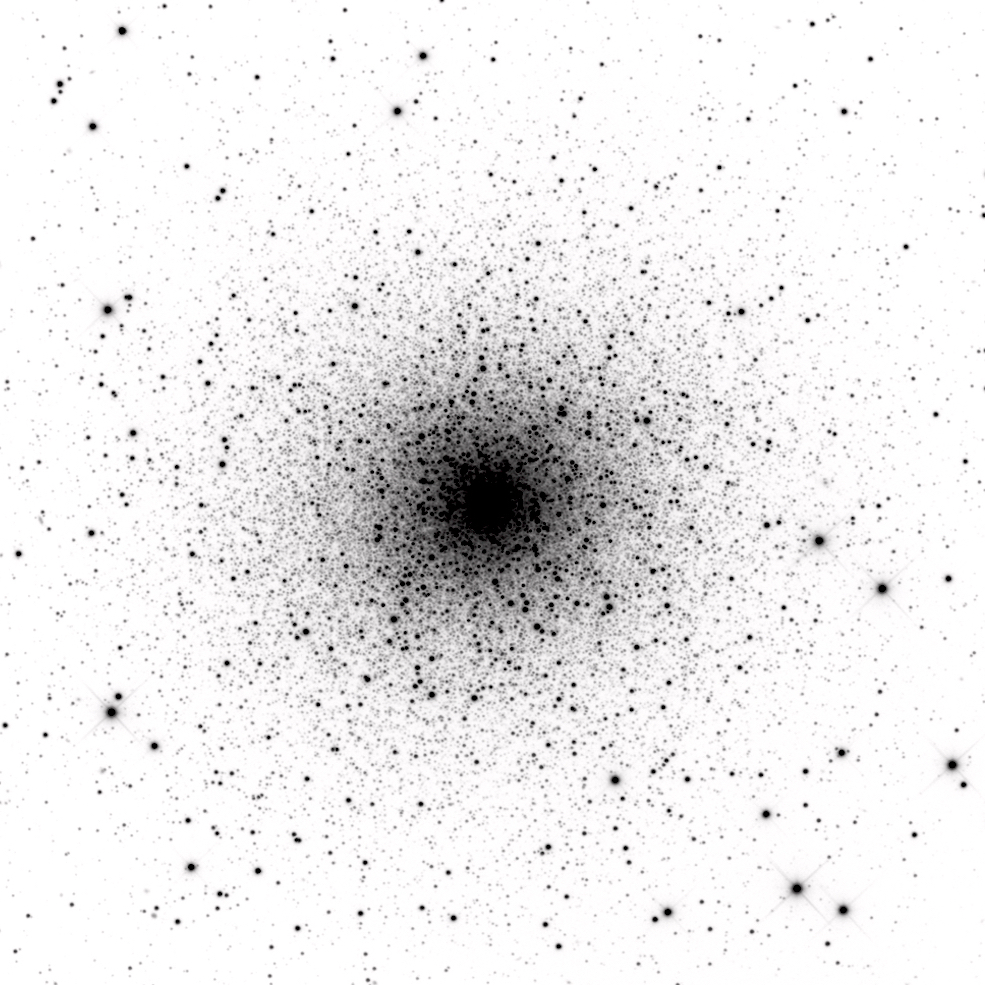
\includegraphics[width = .55\tw]{m13}
	\captionof{figure}{Шаровое скопление M13 (негатив)}
	\vspace{1pc}
	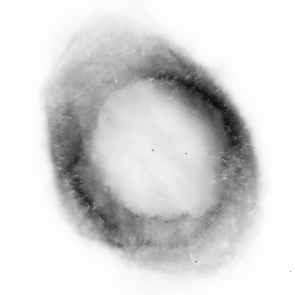
\includegraphics[width = .55\tw]{m57}
	\captionof{figure}{Пла\-не\-тар\-ная туманность M57 (негатив)}
\end{minipage}

\section{Математика}
\subsection{Производная}
\term{Производная в точке}~--- предел отношения приращения функции к приращению её аргумента при стремлении приращения аргумента к нулю, если такой предел существует. \imp{Геометрический смысл производной}: значение производной в точке численно равно тангенсу угла наклона касательной к графику функции в данной точке. Следовательно, точки, где производная обнуляется, соответствуют локальным минимумам и максимумам функции.
\begin{equation}
f^\prime(x_0) = \lim_{\Delta x \to 0}\frac{f(x_0 + \Delta x) - f(x_0)}{\Delta x}
\end{equation}
Общепринятые обозначения для производной функции $y = f(x)$ в точке $x_0$:
\begin{equation}
f^\prime(x_0) = f^\prime_x(x_0) = D f(x_0) = \frac{d f}{d x}(x_0) = \dot{f} (x_0).
\end{equation}
Правила дифференцирования:\\[-0.5pc]
\begin{minipage}{0.5\textwidth}
\begin{align*}
(f+g)^\prime &= f^\prime + g^\prime;\\
(Cf)^\prime &= Cf^\prime;\\
(fg)^\prime &= f^\prime g + f g^\prime;
\end{align*}
\end{minipage}
\begin{minipage}{0.5\textwidth}
\begin{align*}
\left(\dfrac{f}{g}\right)^\prime &= \dfrac{f^\prime g - f g^\prime}{g^2};\\
\dfrac{d}{dx}f\bigl(g(x)\bigr) &= \dfrac{df(g)}{dg}\dfrac{dg(x)}{dx}.
\end{align*}
\end{minipage}\\[0.5pc]
Таблица производных:
\begin{align*} 
(x^a)^\prime &= a x^{a-1};
& (\cos x)^\prime &= - \sin x;
& (\arccos x)^\prime &= - \dfrac{1}{\sqrt{1 - x^2}};\\
(a^x)^\prime &= a^x \ln a;
& (\log_a x)^\prime &= \dfrac{1}{x \ln a}; 
& (\arctg x)^\prime &= \dfrac{1}{1 + x^2};\\
(\sin x)^\prime &= \cos x; 
& (\arcsin x)^\prime &= 
\dfrac{1}{\sqrt{1 - x^2}};
&  (\arcctg x)^\prime &= - \dfrac{1}{1 + x^2}.
\end{align*}
\newpage
\section*{Приложение}

\begin{table}[h!]

\footnotesize
	\renewcommand{\arraystretch}{1.5}
\renewcommand{\tabcolsep}{2pt}
\centering
\begin{tabularx}{\tw}{|C{.13}|C{.125}|C{.14}|C{.125}|C{.115}|C{.15}|C{.13}|}
\hline 
\quad\quad\quad Объект &  Большая полуось  $\mathbf{a}$,~ае & Сиде\-ри\-чес\-кий пе\-риод $\mathbf{T}$,~год & Эксцен\-триситет $\mathbf{e}$ & Накло\-нение $\mathbf{i}$,~$~^\circ$ & Долгота восходящего узла $\mathbf{\Omega}$,~$~^\circ$ & Аргумент перицентра $\mathbf \omega$, $~^\circ$\\
\hline 
Меркурий & 0.387 & 0.241 & 0.206 & 7.0  & 48.3  & 29.1\\ 
 
Венера	 & 0.723 & 0.615 & 0.007 & 3.9  & 76.7  & 54.9\\

Земля    & 1.000 & 1.000 & 0.017 & 0    & 348.7 & 114.\\

Марс     & 1.524 & 1.88  & 0.093 & 1.9  & 49.6  & 286.\\

Церера   & 2.765 & 4.60  & 0.079 & 10.6 & 80.4  & 2.83\\

Юпитер   & 5.204 & 11.86 & 0.048 & 1.0  & 100.6 & 275.\\

Сатурн   & 9.582 & 29.46 & 0.056 & 2.5  & 113.6 & 336.\\

Уран     & 19.23 & 84.01 & 0.044 & 0.8  & 74.0  & 96.5\\

Нептун   & 30.1  & 164.8 & 0.011 & 1.8  & 131.8 & 266.\\

Плутон   & 39.48 & 247.9 & 0.249 & 17.1 & 110.1 & 114.\\ 
 \hline
\end{tabularx}

\end{table}

\begin{table}[h!]

\footnotesize
	\renewcommand{\arraystretch}{1.5}
\renewcommand{\tabcolsep}{2pt}
\centering
\begin{tabularx}{\tw}{|C{0.14}|C{0.16}|C{0.17}|C{0.17}|C{0.17}|C{0.2}|}
\hline  
 Объект &  Обозначение & Масса $\mathbf M$,~кг & Радиус $\mathbf R$,~м & Период $\mathbf T$,~ч & Наклон оси $\mathbf i$,~$~^\circ$\\
\hline 
Солнце & $\odot$ & $1.99 \times 10^{30}$ & $6.97 \times 10^8$ & 609.1 &7.25\\

Меркурий & $\mercury$ & $3.33 \times 10^{23}$ & $2.44 \times 10^6$ & 1408. & 0.035\\ 

Венера   &  $\venus$  & $4.87 \times 10^{24}$ & $6.05 \times 10^6$ & 5833. & 177.4\\

Земля    & $\oplus$   & $5.97 \times 10^{24}$ & $6.37 \times 10^6$ & 23.93 & 23.44 \\

Марс    & $\mars$ & $6.42 \times 10^{23} $ & $3.39 \times 10^6 $  & 24.62 & 25.19 \\

Церера  & \Ceres & $9.39 \times 10^{20}$ & $4.63 \times 10^{5}$  & 9.077 & 3 \\
 
Юпитер   &$\jupiter$ & $1.90 \times 10^{27}$ & $7.00 \times 10^{7}$ & 9.925 & 3.13 \\
 
Сатурн   &$\saturn$& $5.68 \times 10^{26}$ & $5.82 \times 10^{7}$ & 10.53 & 26.73  \\

Уран    & $\uranus$& $8.68 \times 10^{25}$ & $2.54 \times 10^7$ & 17.24 & 97.77  \\

Нептун   &$\neptune$& $1.02 \times 10^{26}$  & $2.46 \times 10^7$ & 15.97 & 28.32  \\

Плутон   &$\pluto$& $1.30 \times 10^{22}$ & $1.19 \times 10^6 $ & 153.3 & 119.6 \\ 
\hline 
\end{tabularx}

\end{table}
\begin{figure}[h!]
	\centering
	\vspace{-.5pc}
	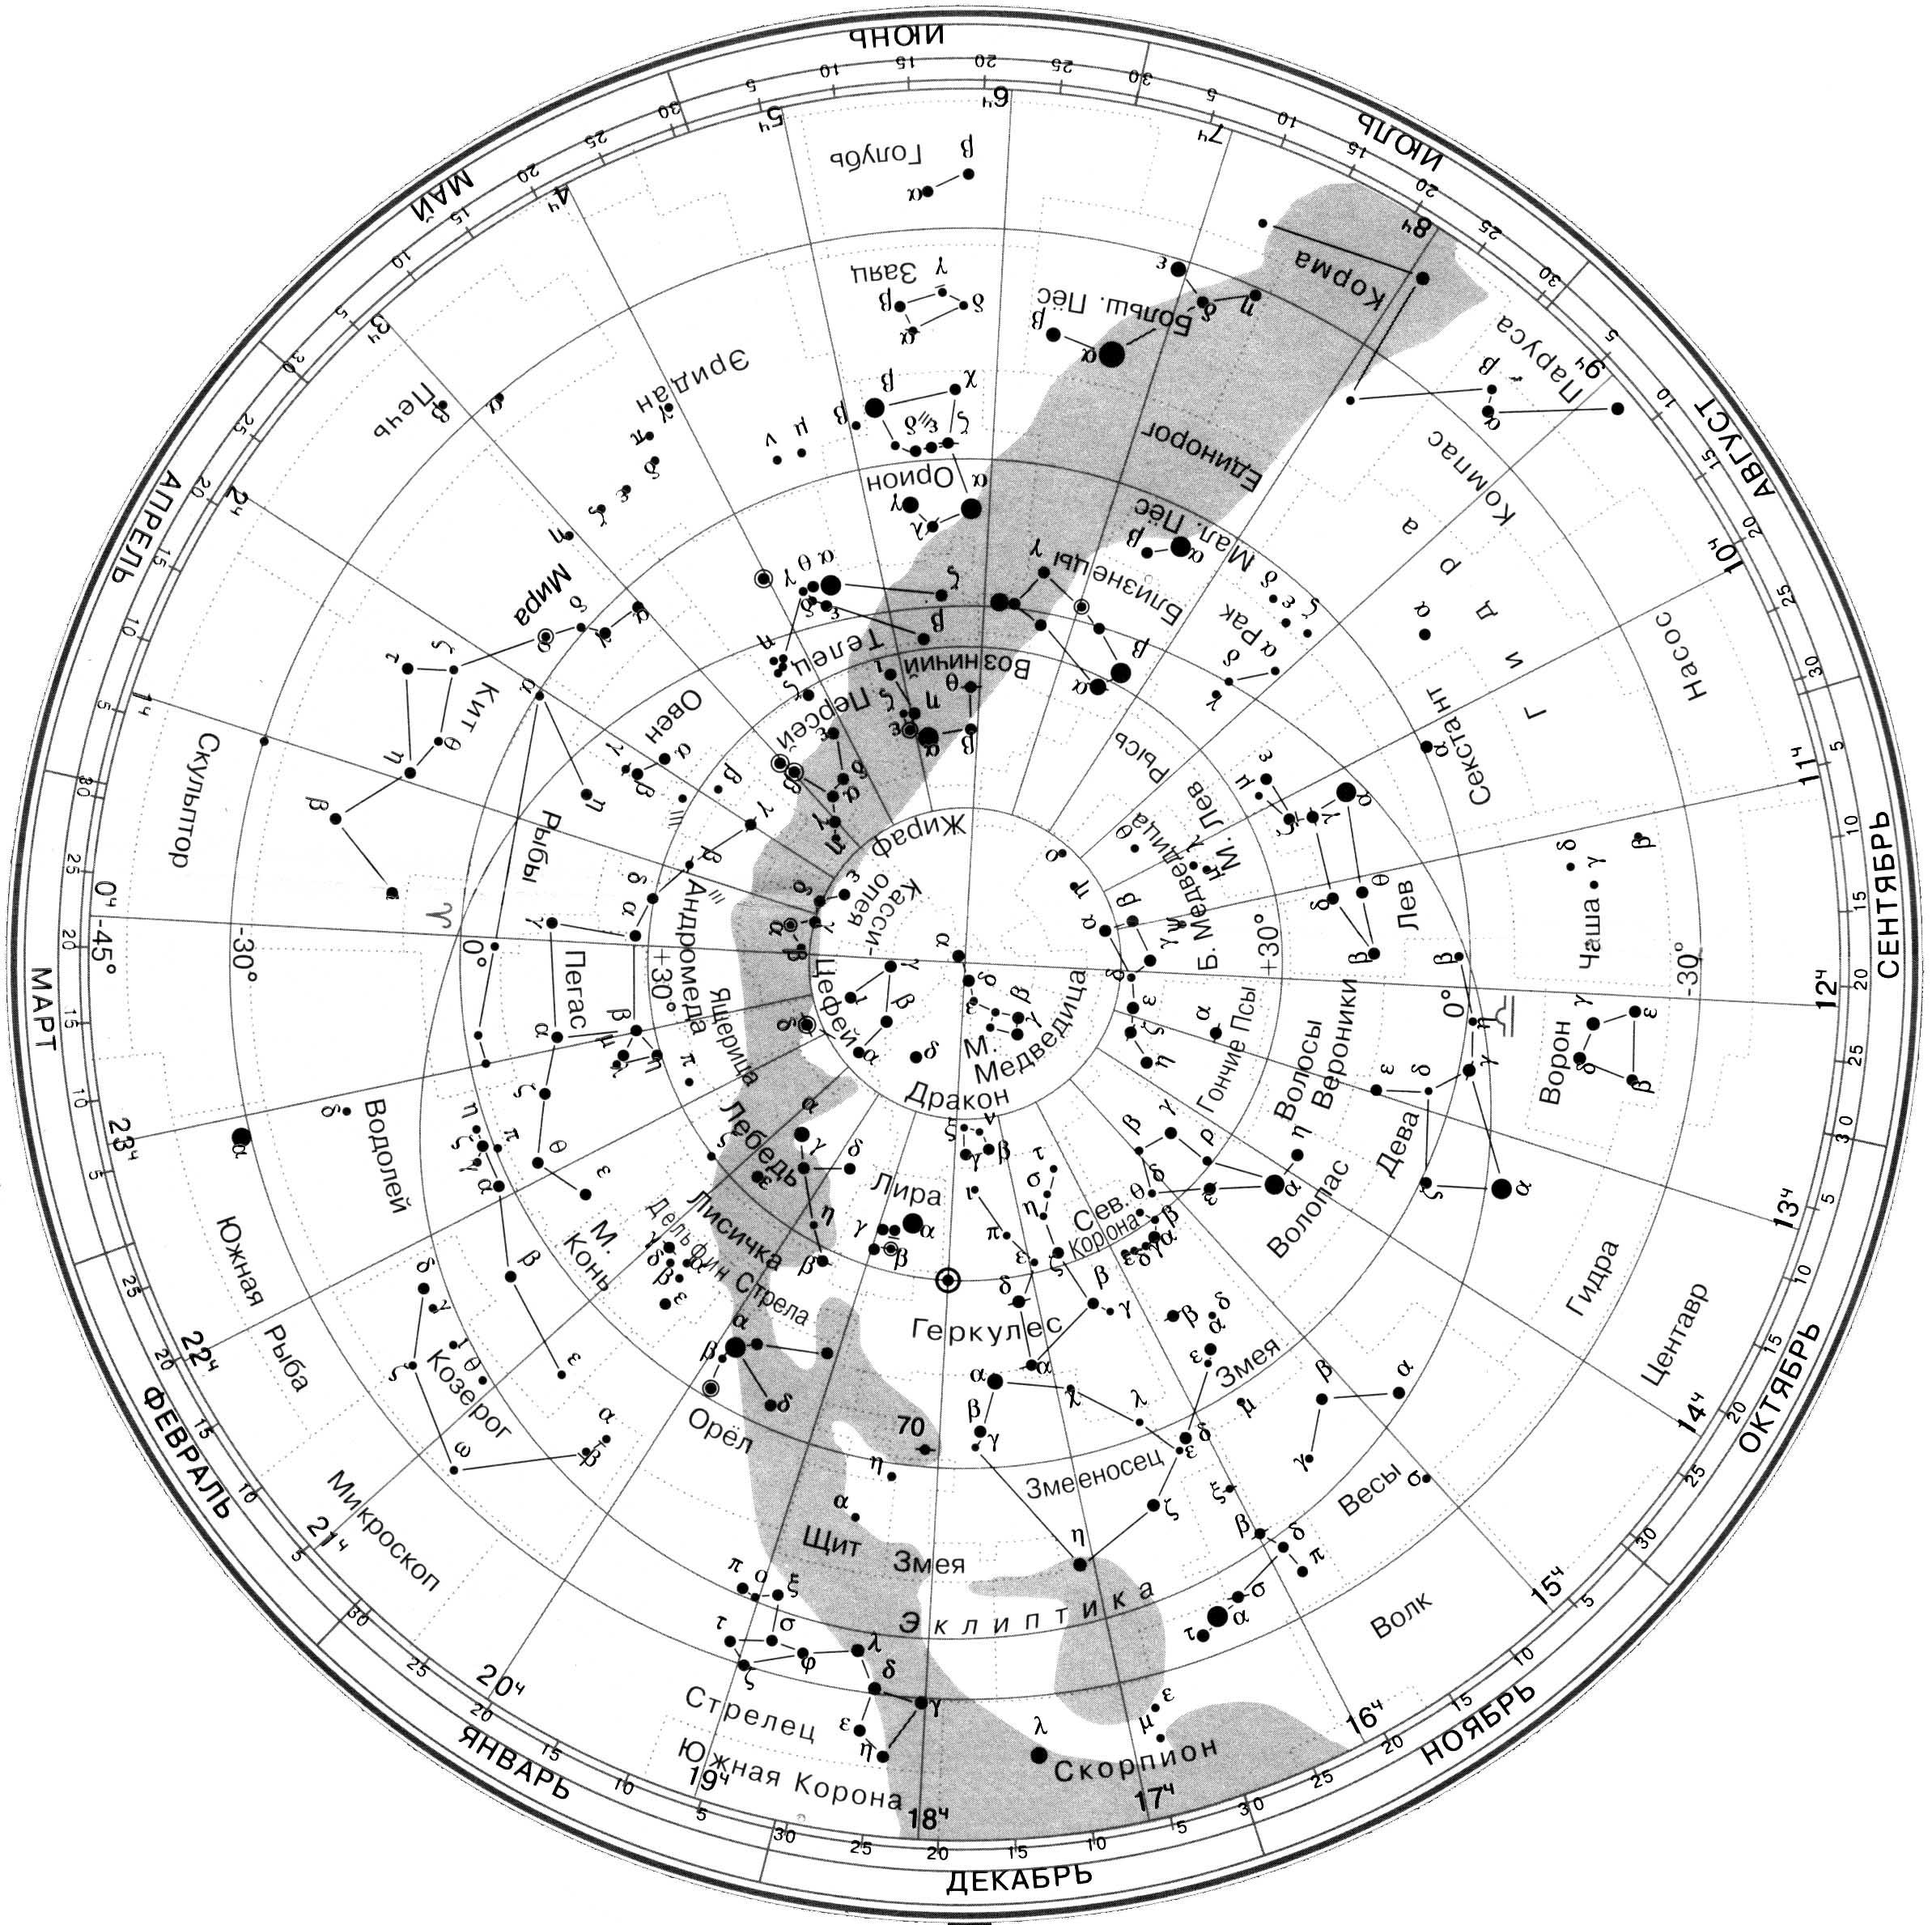
\includegraphics[width=\tw]{sky-map}
	\caption{Карта звёздного неба до $-45^\circ$ по склонению}
	\vspace{-1cm}
\end{figure}
%\newpage
%\thispagestyle{empty}
%\begin{center}
%    { \bfseries \itshape Для заметок}
%\end{center}
\vfill
\newpage
\thispagestyle{empty}
~
\vfill
\centering
\begin{minipage}{0.7\tw}
	\small
	\centering
	Подписано в печать 19.02.2018.\\
	Формат 84$\times$108/32. Бумага офсетная. Печать офсетная.\\
	Тираж 500 экз.\\ 
	Отпечатано в ГУП МО <<Коломенская типография>>.\\ 140400, г.~Коломна, ул.~III Интернационала, д.~2a
\end{minipage}

\newpage
\thispagestyle{empty}
~
\vfill
\centering
\begin{minipage}{0.7\tw}
	\small
	\centering
	Подписано в печать 19.02.2018.\\
	Формат 84$\times$108/32. Бумага офсетная. Печать офсетная.\\
	Тираж 500 экз.\\ 
	Отпечатано в ГУП МО <<Коломенская типография>>.\\ 140400, г.~Коломна, ул.~III Интернационала, д.~2a
\end{minipage}
\end{document}